\documentclass[]{article}

\usepackage{setspace}
\doublespacing

\usepackage[letterpaper, margin=1in]{geometry}


\renewcommand\abstractname{\textit{Abstract}}
\usepackage[cmex10]{amsmath}
\usepackage{amsfonts, amssymb}
\usepackage{color}
\usepackage{bbm}
\usepackage{amsthm}
\usepackage{graphicx}
\usepackage{enumitem}
\graphicspath{{./orth-frame/figure/}{./bi-orth/figure/}}
\makeatletter
\newcommand*{\ov}[1]{\m@th\overline{\mbox{#1}\raisebox{.8em}{}}}
\newcommand{\V}[1]{\boldsymbol{#1}}% boldface for vector and matrix
\usepackage[toc,page]{appendix}
\usepackage{wrapfig}
\usepackage{color}
\usepackage{verbatim}
\usepackage{caption}

\let\oldemptyset\emptyset
\let\emptyset\varnothing
\newcommand{\mo}[1]{m_{#1}(\boldsymbol{\omega})}
\newcommand{\m}[1]{\widetilde{m_{#1}}(\boldsymbol{\omega})}
\renewcommand{\mp}[2]{\widetilde{m_{#1}}(\boldsymbol{\omega}+\boldsymbol{\pi}_{#2})}
\newcommand{\mc}[1]{\widetilde{m_{#1}}^C(\boldsymbol{\omega})}
\newcommand{\barm}[1]{\overline{\widetilde{m_{#1}}(\boldsymbol{\omega})}}
\newcommand{\barmp}[2]{\overline{\widetilde{m_{#1}}(\boldsymbol{\omega} + \boldsymbol{\pi}_{#2})}}
\newcommand{\barmn}[2]{\overline{\widetilde{m_{#1}}(\boldsymbol{\omega} + \boldsymbol{\nu}_{#2})}}
\newcommand{\M}{\widetilde{\mathbf{M}}}
\newcommand{\Msub}{\widetilde{\mathbf{M}}^{\Box}}
\newcommand{\G}{\mathcal{G}}
\newcommand{\mvec}[1]{\mathbf{\widetilde{m_{#1}}}}
\newcommand{\mhat}[1]{\widehat{\widetilde{m_{#1}}}(\boldsymbol{\omega})}
\newcommand{\xvec}{\mathbf{x}}
\newcommand{\wvec}{\mathbf{w}}
\newcommand{\mrow}[1]{\widetilde{\mathbf{m}}^{#1}}
\newtheorem{theorem}{Theorem}[section]
\newtheorem{lemma}[theorem]{Lemma}
\newtheorem{proposition}[theorem]{Proposition}
\newtheorem{corollary}[theorem]{Corollary}
\renewcommand{\qed}{\hfill\ensuremath{\square}}
\newcommand{\mteven}{\overline{\widetilde{\mathbf{m}_0}}^{\mathcal{E}}}
\newcommand{\meven}{\mathbf{m}_0^{\mathcal{E}}}
\newcommand{\mtodd}{\overline{\widetilde{\mathbf{m}_0}}^{\mathcal{O}}}
\newcommand{\modd}{\mathbf{m}_0^{\mathcal{O}}}
\makeatletter

\newcommand{\mylabel}[2]{#2\def\@currentlabel{#2}\label{#1}}
\newcommand*{\overlinespace}[1]{\overline{\mbox{$#1$}\raisebox{3mm}{}}}
\newcommand{\sbarm}[1]{\overlinespace{\widetilde{m_{#1}}}(\boldsymbol{\omega})}
\newcommand{\sbarmp}[2]{\overlinespace{\widetilde{m_{#1}}}(\boldsymbol{\omega} + \boldsymbol{\pi}_{#2})}
\newcommand{\sbarmn}[2]{\overlinespace{\widetilde{m_{#1}}}(\boldsymbol{\omega} + \boldsymbol{\nu}_{#2})}
\makeatother

\begin{document}

\newtheorem{lem}{Lemma}
\newtheorem*{mydef}{Definition}
\newtheorem{thm}{Theorem}
\newtheorem{prop}{Proposition}
\newtheorem*{notat}{Notation}

\abovedisplayskip=2pt
\belowdisplayskip=2pt
\abovedisplayshortskip=2pt
\belowdisplayshortskip=2pt


\title{Directional Wavelet Bases Construction on Dyadic Quincunx Lattice}
\author{Rujie Yin, Ingrid Daubechies}
\maketitle

\begin{abstract}
We construct directional wavelet systems that will enable building efficient signal representation schemes with good direction selectivity. In particular, we focus on wavelet bases on a dyadic quincunx lattice.
%; dilated quincunx downsampling is used to construct orthonormal and bi-orthogonal bases and standard dyadic downsampling for low-redundancy frames. 
In our previous work \cite{yin2014orthshear}, We show that the supports of orthonormal wavelets in our framework are discontinuous in the frequency domain, yet this irregularity constraint can be avoided in frames, even with redundancy factor less than 2. In this paper, we focus on the construction of bi-orthogonal wavelets and show that the same obstruction of regularity as in orthonormal schemes exists in bi-orthogonal schemes. In addition, we provide a numerical algorithm for bi-orthogonal wavelets construction that reveals its intrinsic irregularity.
\end{abstract}

\section{Introduction}

\iffalse
\begin{itemize}
\item review construction of directional wavelet, shearlet
\item what's new in our construction?
\item summary: framework, technique, reference(Durand, Cohen)
\item organization of the paper
\end{itemize}
\fi

% introducing directional wavelets
In image compression and analysis, 2D tensor wavelet schemes are widely used. Despite the time-frequency localization inherited from 1D wavelet, 2D tensor wavelets suffer from poor orientation selectivity: only horizontal or vertical edges are well represented by tensor wavelets. To obtain better representation of 2D images, several directional wavelet schemes have been proposed and applied to image processing, such as directional wavelet filterbanks (DFB) and various extensions.

% summary
Conventional DFB \cite{DFB92} divides the square frequency domain associated with a regular 2D lattice into eight equi-angular pairs of triangles; such schemes can be critically downsampled (maximally decimated) with perfect reconstruction (PR), but they typically do not have a multi-resolution structure. 
Different approaches have been proposed to generalize DFB to multi-resolution systems, including non-uniform DFB (nuDFB), contourlets, curvelets, shearlets and dual-tree wavelets.
nuDFB is introduced in \cite{nuDFB05} based on multi-resolution analysis (MRA), where at each level of decomposition the square frequency domain is divided into a high frequency outer ring and a central low frequency domain. For nuDFB, the high frequency ring is primarily divided further into six equi-angular pairs of trapezoids and the central low frequency square is kept intact for division in the next level of decomposition, see the left panel in Figure \ref{fig: partition}. The nuDFB filters are solved by optimization which provides non-unique near orthogonal or bi-orthogonal solutions depending on the initialization without stable convergence.
Contourlets \cite{do2005contourlet} combine the Laplacian pyramid scheme with DFB which has PR but with redundancy $4/3$ inherited from the Laplacian pyramid.
Shearlet \cite{shearlet12book,easley2008sparse} and curvelet \cite{candes2006fast} systems construct a multi-resolution partition of the frequency domain by applying shear or rotation operators to a generator function in each level of frequency decomposition. Available shearlet and curvelet implementations have redundancy at least 4; moreover, the factor may grow with the number of directions in the decomposition level.
% to be modified and add M-band version
Dual-tree wavelets \cite{selesnick2005dual} are linear combinations of 2D tensor wavelets (corresponding to multi-resolution systems) that constitute an approximate Hilbert transform pair, where the high frequency ring is divided into pairs of squares of different directional preference.

% what's the problem we will address, don't focusing too much on shearlet for the moment
However, none of these multi-resolution schemes is PR, critically downsampled and regularized (localized in both time and frequency). In the framework of nuDFB (\cite{nuDFB05}), it was shown by Durand \cite{durand2007} that it is impossible to construct orthonormal filters localize without discontinuity in the frequency domain, or -- equivalently -- regularized filters without aliasing. His construction of directional filters uses compositions of 2-band filters associated to quincunx lattice, similar to that of uniform DFB in \cite{nuDFB05}; as pointed out in \cite{nuDFB05} the overall composed filters are not alias-free. It is not clear whether Durand's argument also precludes the existence of a regularized wavelet system, if one slightly weakens the set of conditions.
%Among these,  shearlets and curvelets have optimal asymptotic rate of approximation for ``cartoon images''(piecewise smooth, with jumps occurring along piecewise $C^2$-curves), due to the parabolic scaling rule in the frequency domain \cite{guo2007optimally,candes2005curvelet}; they have been successfully applied to image denoising \cite{easley2009shearlet}, restoration \cite{candes2002new} and separation \cite{kutyniok2012image}. Despite their theoretical potential, the (often high) redundancy of curvelets and shearlets impedes their practical usage. 
%Redundancy is useful in image processing tasks such as denoising, restoration and reconstruction, but a non-redundant basis decomposition is preferred in tasks where computation cost is of concern.

To study this question, we consider multi-resolution directional wavelets corresponding to the same partition of frequency domain as nuDFB and build a framework to analyze the equivalent conditions of PR for critically downsampled as well as more general redundant schemes. In our previous work \cite{yin2014orthshear}, we show that in MRA on a dyadic quincunx lattice, PR is equivalent to an identity condition and a set of shift-cancellation conditions closely related to the frequency support of filters and their downsampling scheme. Based on these two conditions, we rederived Durand's discontinuity result of orthonormal schemes; we also show that a slight relaxation of conditions allows frames with redundancy less than 2 that circumvent the regularity limitation. Furthermore, we have an explicit approach to construct such regularized directional wavelet frames by smoothing the Fourier transform of the irregular directional wavelets.
The main contribution of this paper is that we extend our previous work and show that the same obstruction to regularity as in orthonormal schemes exists in biorthogonal schemes. Different from our previous approach in the orthonormal case, our analysis of bi-orthogonal schemes is inspired by Cohen et al's approach in \cite{cohen1993compactly} for numerical construction of compactly supported symmetric wavelet bases on a hexagonal lattice. We extend and adapt their numerical construction to our bi-orthogonal setting.

The paper is organized as follows. In Section \ref{sec: setup}, we set up the framework of an MRA with dyadic quincunx downsampling. In Section \ref{sec: orth}, we review the regularity analysis of orthonormal schemes and its extension to frames in \cite{yin2014orthshear}. In particular, we derive two conditions, {\it identity summation} and {\it shift cancellation}, equivalent to perfect reconstruction in this MRA with critical downsampling. These lead to the classification of {\it regular/singular} boundaries of the frequency partition %and the corresponding smoothing techniques to improve spatial localization. We compare our and Durand's directional wavelet constructions. 
%In section \ref{sec: frame}, 
and a {\it relaxed shift-cancellation} condition for low-redundancy MRA frame allows better regularity of the directional wavelets. 
In Section \ref{sec: bi-orth}, we extend the orthonormal schemes to biorthogonal schemes as well as the corresponding {\it identity summation} and {\it shift cancellation} conditions. We then introduce Cohen et al's approach in \cite{cohen1993compactly} and adapt it to the regularity analysis on our biorthogonal schemes due to these conditions. We show that the biorthogonal schemes have the same irregularity as in the orthonormal schemes.
In Section \ref{sec: solve-quincunx}, we  propose a numerical algorithm for the construction of biorthogonal schemes along with further analysis on the regularity constraints.
%the resulting linear system does not have feasible solution satisfying all regularity constraints, especially continuity of Fourier transforms of wavelet filters.  
Finally, we present and discuss numerical results of our algorithm in Section \ref{sec: numerics}, and conclude our current work in Section \ref{sec: end}.

%\section{Introduction}

\iffalse
\begin{itemize}
\item review construction of directional wavelet, shearlet
\item what's new in our construction?
\item summary: framework, technique, reference(Durand, Cohen)
\item organization of the paper
\end{itemize}
\fi

% introducing directional wavelets
In image compression and analysis, 2D tensor wavelet schemes are widely used. Despite the time-frequency localization inherited from 1D wavelet, 2D tensor wavelets suffer from poor orientation selectivity: only horizontal or vertical edges are well represented by tensor wavelets. To obtain better representation of 2D images, several directional wavelet schemes have been proposed and applied to image processing, such as directional wavelet filterbanks (DFB) and various extensions.

% summary
Conventional DFB \cite{DFB92} divides the square frequency domain associated with a regular 2D lattice into eight equi-angular pairs of triangles; such schemes can be critically downsampled (maximally decimated) with perfect reconstruction (PR), but they typically do not have a multi-resolution structure. 
Different approaches have been proposed to generalize DFB to multi-resolution systems, including non-uniform DFB (nuDFB), contourlets, curvelets, shearlets and dual-tree wavelets.
nuDFB is introduced in \cite{nuDFB05} based on multi-resolution analysis (MRA), where at each level of decomposition the square frequency domain is divided into a high frequency outer ring and a central low frequency domain. For nuDFB, the high frequency ring is primarily divided further into six equi-angular pairs of trapezoids and the central low frequency square is kept intact for division in the next level of decomposition, see the left panel in Figure \ref{fig: partition}. The nuDFB filters are solved by optimization which provides non-unique near orthogonal or bi-orthogonal solutions depending on the initialization without stable convergence.
Contourlets \cite{do2005contourlet} combine the Laplacian pyramid scheme with DFB which has PR but with redundancy $4/3$ inherited from the Laplacian pyramid.
Shearlet \cite{shearlet12book,easley2008sparse} and curvelet \cite{candes2006fast} systems construct a multi-resolution partition of the frequency domain by applying shear or rotation operators to a generator function in each level of frequency decomposition. Available shearlet and curvelet implementations have redundancy at least 4; moreover, the factor may grow with the number of directions in the decomposition level.
% to be modified and add M-band version
Dual-tree wavelets \cite{selesnick2005dual} are linear combinations of 2D tensor wavelets (corresponding to multi-resolution systems) that constitute an approximate Hilbert transform pair, where the high frequency ring is divided into pairs of squares of different directional preference.

% what's the problem we will address, don't focusing too much on shearlet for the moment
However, none of these multi-resolution schemes is PR, critically downsampled and regularized (localized in both time and frequency). In the framework of nuDFB (\cite{nuDFB05}), it was shown by Durand \cite{durand2007} that it is impossible to construct orthonormal filters localize without discontinuity in the frequency domain, or -- equivalently -- regularized filters without aliasing. His construction of directional filters uses compositions of 2-band filters associated to quincunx lattice, similar to that of uniform DFB in \cite{nuDFB05}; as pointed out in \cite{nuDFB05} the overall composed filters are not alias-free. It is not clear whether Durand's argument also precludes the existence of a regularized wavelet system, if one slightly weakens the set of conditions.
%Among these,  shearlets and curvelets have optimal asymptotic rate of approximation for ``cartoon images''(piecewise smooth, with jumps occurring along piecewise $C^2$-curves), due to the parabolic scaling rule in the frequency domain \cite{guo2007optimally,candes2005curvelet}; they have been successfully applied to image denoising \cite{easley2009shearlet}, restoration \cite{candes2002new} and separation \cite{kutyniok2012image}. Despite their theoretical potential, the (often high) redundancy of curvelets and shearlets impedes their practical usage. 
%Redundancy is useful in image processing tasks such as denoising, restoration and reconstruction, but a non-redundant basis decomposition is preferred in tasks where computation cost is of concern.

To study this question, we consider multi-resolution directional wavelets corresponding to the same partition of frequency domain as nuDFB and build a framework to analyze the equivalent conditions of PR for critically downsampled as well as more general redundant schemes. In our previous work \cite{yin2014orthshear}, we show that in MRA on a dyadic quincunx lattice, PR is equivalent to an identity condition and a set of shift-cancellation conditions closely related to the frequency support of filters and their downsampling scheme. Based on these two conditions, we rederived Durand's discontinuity result of orthonormal schemes; we also show that a slight relaxation of conditions allows frames with redundancy less than 2 that circumvent the regularity limitation. Furthermore, we have an explicit approach to construct such regularized directional wavelet frames by smoothing the Fourier transform of the irregular directional wavelets.
The main contribution of this paper is that we extend our previous work and show that the same obstruction to regularity as in orthonormal schemes exists in biorthogonal schemes. Different from our previous approach in the orthonormal case, our analysis of bi-orthogonal schemes is inspired by Cohen et al's approach in \cite{cohen1993compactly} for numerical construction of compactly supported symmetric wavelet bases on a hexagonal lattice. We extend and adapt their numerical construction to our bi-orthogonal setting.

The paper is organized as follows. In Section \ref{sec: setup}, we set up the framework of an MRA with dyadic quincunx downsampling. In Section \ref{sec: orth}, we review the regularity analysis of orthonormal schemes and its extension to frames in \cite{yin2014orthshear}. In particular, we derive two conditions, {\it identity summation} and {\it shift cancellation}, equivalent to perfect reconstruction in this MRA with critical downsampling. These lead to the classification of {\it regular/singular} boundaries of the frequency partition %and the corresponding smoothing techniques to improve spatial localization. We compare our and Durand's directional wavelet constructions. 
%In section \ref{sec: frame}, 
and a {\it relaxed shift-cancellation} condition for low-redundancy MRA frame allows better regularity of the directional wavelets. 
In Section \ref{sec: bi-orth}, we extend the orthonormal schemes to biorthogonal schemes as well as the corresponding {\it identity summation} and {\it shift cancellation} conditions. We then introduce Cohen et al's approach in \cite{cohen1993compactly} and adapt it to the regularity analysis on our biorthogonal schemes due to these conditions. We show that the biorthogonal schemes have the same irregularity as in the orthonormal schemes.
In Section \ref{sec: solve-quincunx}, we  propose a numerical algorithm for the construction of biorthogonal schemes along with further analysis on the regularity constraints.
%the resulting linear system does not have feasible solution satisfying all regularity constraints, especially continuity of Fourier transforms of wavelet filters.  
Finally, we present and discuss numerical results of our algorithm in Section \ref{sec: numerics}, and conclude our current work in Section \ref{sec: end}.
%\section{Introduction}

\iffalse
\begin{itemize}
\item review construction of directional wavelet, shearlet
\item what's new in our construction?
\item summary: framework, technique, reference(Durand, Cohen)
\item organization of the paper
\end{itemize}
\fi

% introducing directional wavelets
In image compression and analysis, 2D tensor wavelet schemes are widely used. Despite the time-frequency localization inherited from 1D wavelet, 2D tensor wavelets suffer from poor orientation selectivity: only horizontal or vertical edges are well represented by tensor wavelets. To obtain better representation of 2D images, several directional wavelet schemes have been proposed and applied to image processing, such as directional wavelet filterbanks (DFB) and various extensions.

% summary
Conventional DFB \cite{DFB92} divides the square frequency domain associated with a regular 2D lattice into eight equi-angular pairs of triangles; such schemes can be critically downsampled (maximally decimated) with perfect reconstruction (PR), but they typically do not have a multi-resolution structure. 
Different approaches have been proposed to generalize DFB to multi-resolution systems, including non-uniform DFB (nuDFB), contourlets, curvelets, shearlets and dual-tree wavelets.
nuDFB is introduced in \cite{nuDFB05} based on multi-resolution analysis (MRA), where at each level of decomposition the square frequency domain is divided into a high frequency outer ring and a central low frequency domain. For nuDFB, the high frequency ring is primarily divided further into six equi-angular pairs of trapezoids and the central low frequency square is kept intact for division in the next level of decomposition, see the left panel in Figure \ref{fig: partition}. The nuDFB filters are solved by optimization which provides non-unique near orthogonal or bi-orthogonal solutions depending on the initialization without stable convergence.
Contourlets \cite{do2005contourlet} combine the Laplacian pyramid scheme with DFB which has PR but with redundancy $4/3$ inherited from the Laplacian pyramid.
Shearlet \cite{shearlet12book,easley2008sparse} and curvelet \cite{candes2006fast} systems construct a multi-resolution partition of the frequency domain by applying shear or rotation operators to a generator function in each level of frequency decomposition. Available shearlet and curvelet implementations have redundancy at least 4; moreover, the factor may grow with the number of directions in the decomposition level.
% to be modified and add M-band version
Dual-tree wavelets \cite{selesnick2005dual} are linear combinations of 2D tensor wavelets (corresponding to multi-resolution systems) that constitute an approximate Hilbert transform pair, where the high frequency ring is divided into pairs of squares of different directional preference.

% what's the problem we will address, don't focusing too much on shearlet for the moment
However, none of these multi-resolution schemes is PR, critically downsampled and regularized (localized in both time and frequency). In the framework of nuDFB (\cite{nuDFB05}), it was shown by Durand \cite{durand2007} that it is impossible to construct orthonormal filters localize without discontinuity in the frequency domain, or -- equivalently -- regularized filters without aliasing. His construction of directional filters uses compositions of 2-band filters associated to quincunx lattice, similar to that of uniform DFB in \cite{nuDFB05}; as pointed out in \cite{nuDFB05} the overall composed filters are not alias-free. It is not clear whether Durand's argument also precludes the existence of a regularized wavelet system, if one slightly weakens the set of conditions.
%Among these,  shearlets and curvelets have optimal asymptotic rate of approximation for ``cartoon images''(piecewise smooth, with jumps occurring along piecewise $C^2$-curves), due to the parabolic scaling rule in the frequency domain \cite{guo2007optimally,candes2005curvelet}; they have been successfully applied to image denoising \cite{easley2009shearlet}, restoration \cite{candes2002new} and separation \cite{kutyniok2012image}. Despite their theoretical potential, the (often high) redundancy of curvelets and shearlets impedes their practical usage. 
%Redundancy is useful in image processing tasks such as denoising, restoration and reconstruction, but a non-redundant basis decomposition is preferred in tasks where computation cost is of concern.

To study this question, we consider multi-resolution directional wavelets corresponding to the same partition of frequency domain as nuDFB and build a framework to analyze the equivalent conditions of PR for critically downsampled as well as more general redundant schemes. In our previous work \cite{yin2014orthshear}, we show that in MRA on a dyadic quincunx lattice, PR is equivalent to an identity condition and a set of shift-cancellation conditions closely related to the frequency support of filters and their downsampling scheme. Based on these two conditions, we rederived Durand's discontinuity result of orthonormal schemes; we also show that a slight relaxation of conditions allows frames with redundancy less than 2 that circumvent the regularity limitation. Furthermore, we have an explicit approach to construct such regularized directional wavelet frames by smoothing the Fourier transform of the irregular directional wavelets.
The main contribution of this paper is that we extend our previous work and show that the same obstruction to regularity as in orthonormal schemes exists in biorthogonal schemes. Different from our previous approach in the orthonormal case, our analysis of bi-orthogonal schemes is inspired by Cohen et al's approach in \cite{cohen1993compactly} for numerical construction of compactly supported symmetric wavelet bases on a hexagonal lattice. We extend and adapt their numerical construction to our bi-orthogonal setting.

The paper is organized as follows. In Section \ref{sec: setup}, we set up the framework of an MRA with dyadic quincunx downsampling. In Section \ref{sec: orth}, we review the regularity analysis of orthonormal schemes and its extension to frames in \cite{yin2014orthshear}. In particular, we derive two conditions, {\it identity summation} and {\it shift cancellation}, equivalent to perfect reconstruction in this MRA with critical downsampling. These lead to the classification of {\it regular/singular} boundaries of the frequency partition %and the corresponding smoothing techniques to improve spatial localization. We compare our and Durand's directional wavelet constructions. 
%In section \ref{sec: frame}, 
and a {\it relaxed shift-cancellation} condition for low-redundancy MRA frame allows better regularity of the directional wavelets. 
In Section \ref{sec: bi-orth}, we extend the orthonormal schemes to biorthogonal schemes as well as the corresponding {\it identity summation} and {\it shift cancellation} conditions. We then introduce Cohen et al's approach in \cite{cohen1993compactly} and adapt it to the regularity analysis on our biorthogonal schemes due to these conditions. We show that the biorthogonal schemes have the same irregularity as in the orthonormal schemes.
In Section \ref{sec: solve-quincunx}, we  propose a numerical algorithm for the construction of biorthogonal schemes along with further analysis on the regularity constraints.
%the resulting linear system does not have feasible solution satisfying all regularity constraints, especially continuity of Fourier transforms of wavelet filters.  
Finally, we present and discuss numerical results of our algorithm in Section \ref{sec: numerics}, and conclude our current work in Section \ref{sec: end}.


\section{Framework Setup}\label{sec: setup}
We summarize 2D-MRA systems and the relation between frequency domain partition and sub-lattice of $\mathbb{Z}^2$ with critical downsampling following \cite{yin2014orthshear}.

\subsection{Notation}
Throughout this paper, we use lower case normal font for function, upper case bold font for matrix, lower case bold font for vector and upper case normal font for frequency domain. We denote the conjugate transpose of a matrix $\V{A}$ by $\V{A}^*$ and same for a vector.

\subsection{Multi-resolution analysis and sub-lattice sampling}
In an MRA, given a scaling function $\phi\in L^2(\mathbb{R}^2)$, s.t. $\Vert\phi\Vert_2=1$,
the base approximation space is defined as $V_0 = \overline{span\{\phi_{0,\boldsymbol{k}}\}}_{\boldsymbol{k}\in\mathbb{Z}^2}$, where $\phi_{0,\boldsymbol{k}} = \phi(\boldsymbol{x}-\boldsymbol{k})$. If $\langle \phi_{0,\boldsymbol{k}},\phi_{0,\boldsymbol{k'}}\rangle = \delta_{\boldsymbol{k,k'}}$, then $\{\phi_{0,\boldsymbol{k}}\}$ is an orthonormal basis of $V_0$. In addition, $\phi$ is associated with a scaling matrix $\mathbf{D}\in\mathbb{Z}^{2\times 2}$, s.t. the dilated scaling function
 $\phi_1(\boldsymbol{x}) = |\mathbf{D}|^{-1/2}\phi(\mathbf{D}^{-1}\boldsymbol{x})$ is a linear combination of $\phi_{0,\boldsymbol{k}}$'s.
Equivalently, $\exists\,m_0(\boldsymbol{\omega}) = m_0(\omega_1,\omega_2)$, $2\pi-$periodic in $\omega_1,\omega_2$, s.t. in the frequency domain
\begin{align}\label{eq: m0}
\widehat{\phi}(\mathbf{D}^T\boldsymbol{\omega}) = m_0(\boldsymbol{\omega})\widehat{\phi}(\boldsymbol{\omega}).
\end{align}
\eqref{eq: m0} implies that
\begin{align}\label{eq: phi-m0}
\textstyle \hat{\phi}(\boldsymbol{\omega}) = (2\pi)^{-1}\prod_{k=1}^{\infty}m_0(\mathbf{D}^{-k} \boldsymbol{\omega}).
\end{align}
\\[.2em]
Let $\phi_{l,\boldsymbol{k}} = \phi(D^{-l}\boldsymbol{x}-\boldsymbol{k})$
and $V_l = \overline{span\{\phi_{l,\boldsymbol{k}};\boldsymbol{k}\in\mathbb{Z}^2\}},\,l\in\mathbb{Z}$ be the nested approximation spaces. Define $W_l$ as the orthogonal complement of $V_l$ with respect to $V_{l-1}$ in MRA. 
Suppose there are $J$ wavelet functions $\psi^j\in L^2(\mathbb{R}^2)$, {\small $1 \leq j \leq J$}, and $\mathbf{Q}\in\mathbb{Z}^{2\times2}$, s.t.
\begin{align*}
\hspace{-1em} W_1 = \bigcup_{j=1}^J W_1^j = \bigcup_{j=1}^J \overline{span\{\psi^j_{1,\boldsymbol{k}};\boldsymbol{ k}\in \mathbf{Q}\mathbb{Z}^2\}}= \bigcup_{j=1}^J \overline{span\{\psi^j(\mathbf{D}^{-1}\boldsymbol{x-k});\boldsymbol{ k}\in \mathbf{Q}\mathbb{Z}^2\}},
\end{align*}
 an $L$-level multi-resolution system with base space $V_0$ is then spanned by
 \begin{align}\label{eq: MRA}
 V_L\oplus\,\bigoplus_{l=1}^L\Big(\bigcup_{j=1}^J\, W_l^j\Big) =
 \{\phi_{L,\boldsymbol{k}}\,,\psi^j_{l,\boldsymbol{k'}}\,, \, {\small 1\leq l \leq L,\, \boldsymbol{k}\in \mathbb{Z}^2,\,\boldsymbol{k'}\in \mathbf{Q}\mathbb{Z}^2,\,1\leq j \leq J\}}.
\end{align}  
In particular, we set $\mathbf{D} = \mathbf{D_2}\doteq\bigl(\begin{smallmatrix} 2&0\\0&2\end{smallmatrix}\bigr)$ and $\mathbf{Q}:=\bigl(\begin{smallmatrix} 1&1\\-1&1\end{smallmatrix}\bigr)$.
As $W_1\subset V_0$, each rescaled wavelet $\psi^j(\mathbf{D}^{-1}\cdot)$ is also a linear combination of $\phi_{0,\boldsymbol{k}}$, so that $\exists\, m_j$ analogous to $m_0$
satisfying 
\begin{align}\label{eq: mj}
\widehat{\psi}^j(\mathbf{D}^T\boldsymbol{\omega}) = m_j(\boldsymbol{\omega})\widehat{\phi}(\boldsymbol{\omega}),\hspace{1cm} 1\leq j \leq J.
\end{align}
In this specific construction of MRA,
% the scaling function $\phi$ and all the wavelet functions $\psi^j$ share the same scaling matrix $\mathbf{D}$, yet the family of shifted $\phi_{\boldsymbol{k}}$ is defined on $\mathbb{Z}^2$, whereas the family of shifted $\psi^j_{\boldsymbol{k}}$ is defined on a sub-integer lattice $\mathbf{Q}\mathbb{Z}^2$. Hence 
 the corresponding subsampling matrix of $\phi_{1,\boldsymbol{k}}$ is $\mathbf{D}$ and that of $\psi^j_{1,\boldsymbol{k}}$ is $\mathbf{QD}$, the dilated quincunx subsample (see the right panel in Fig.\ref{fig: partition}), as in \cite{durand2007}. 
% We haven't yet imposed any condition on this MRA, or equivalently, on $m-$functions and the subsampling matrices $\mathbf{D}$ and $\mathbf{Q}$; this comes next.


\subsection{Frequency domain partition and critical downsampling}

%critical downsampling thus depends only on the subsampling matrices $\mathbf{D}$ and $\mathbf{Q}$. The space decomposition structure $V_0 = V_1\bigoplus W_1$ in MRA and \eqref{eq: m0}, \eqref{eq: mj} require consistency between the $m-$functions and the subsampling matrices $\mathbf{D}$ and $\mathbf{Q}$. 

\begin{figure}[!t]
\centering
\begin{minipage}[c]{.42\textwidth}
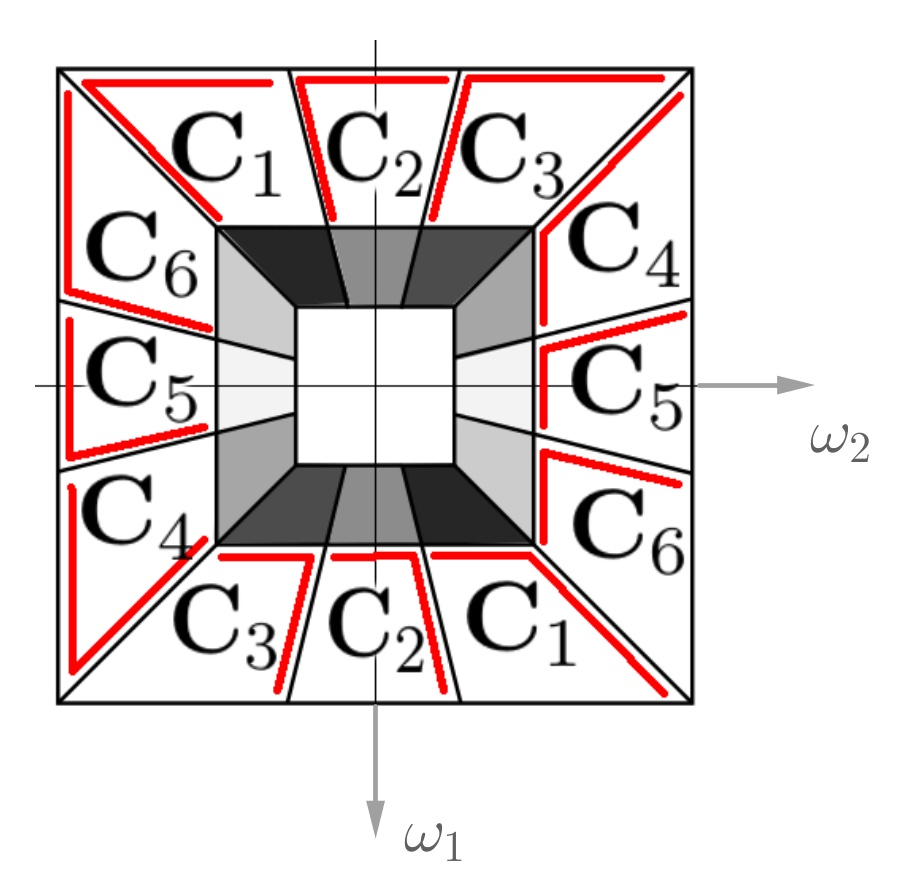
\includegraphics[width=\textwidth]{shannon-marked-wcoord.jpg}
\end{minipage}\hspace*{3em}
\begin{minipage}[c]{.3\textwidth}
\includegraphics[width=\textwidth]{sublattice-2.jpg}
\vspace*{1em}
\end{minipage}
\caption{Left: partition of $S_0$ and boundary assignment of $C_j$, $j = 1,\cdots,6$ ( each $C_j$ has boundaries indicated by red line segments), Right: dilated quincunx sub-lattice. }
\label{fig: partition}
\vspace*{-5mm}
\end{figure}

%\begin{mydef}
%If $\mathcal{L}$ is the lattice generated by $\boldsymbol{a}_1,\boldsymbol{a}_2$, i.e. $\mathcal{L} = \sum_{i=1,2}k_i\boldsymbol{a}_i,\,k_i\in\mathbb{Z}$,the {\bf reciprocal lattice} $\mathcal{L}^*$ of $\mathcal{L}$ is the lattice generated by the vectors $\boldsymbol{b}_1,\boldsymbol{b}_2$, s.t. $\boldsymbol{b}_i^T\boldsymbol{a}_j = 2\pi\delta_{ij}$. 
%\end{mydef}

%\begin{mydef}
%Given a lattice $\mathcal{L}$, a {\bf fundamental domain} $S$ in $\mathbb{R}^2$ with respect to $\mathcal{L}$, denoted as $S = \mathbb{R}^2/\mathcal{L}$, is a subset of $\mathbb{R}^2$, such that $\bigcup_{l\in\mathcal{L}}(S+l) = \mathbb{R}^2$ and $S\cap(S+l)=\varnothing,\,\forall l\in\mathcal{L}\setminus\{\mathbf{0}\}$.
%A set $S$ is a {\bf frequency support} of $\mathcal{L}$ if $S = \mathbb{R}^2/\mathcal{L}^*$.
%\end{mydef}
%Furthermore, each sub-lattice $\mathcal{L}$ of $\mathbb{Z}^2$ is associated with a set of shifts $\Gamma, \, s.t. \bigcup_{\V{\gamma}\in\Gamma}\mathcal{L}+\V{\gamma} = \mathbb{Z}^2$ and $|\Gamma| = |\mathbb{Z}^2/\mathcal{L}|$.

Consider the canonical frequency square, $S_0 = [-\pi,\pi)\times[-\pi,\pi)$ associated with lattice $\mathcal{L} = \mathbb{Z}^2$. 
%Due to \eqref{eq: m0} and \eqref{eq: mj}, this is equivalent to $S_0=\bigcup_{0\leq j\leq J} supp(m_j\vert_{S_0})$.That is, 
Consider a 1-level decomposition, \eqref{eq: MRA} together with \eqref{eq: m0} and \eqref{eq: mj} implies that the union of the support of $m_j,\,0\leq j\leq J$ covers $S_0$.
Furthermore, $\exists\, C_j\subset supp(m_j), 0\leq j\leq J,$ such that they form a partition of $S_0$, and it is natural to take $C_j$ as the main support of $m_j$.
To build an orthonormal basis with good directional selectivity, we choose the partition of $S_0$ shown in the left of Fig.\ref{fig: partition}, which is the same for Example B in \cite{durand2007} and the least redundant shearlet system. In this partition, $S_0$ is divided into a central square $C_0 = \bigl(\begin{smallmatrix} 2&0\\0&2\end{smallmatrix}\bigr)^{-1}S_0$ and a ring: the ring is further cut into six pairs of directional trapezoids $C_j$'s by lines passing through the origin with slopes $\pm 1, \pm 3$ and $\pm \frac{1}{3}$. The central square $C_0$ can be further partitioned in the same way to obtain a two-level multi-resolution system, as shown in Fig.\ref{fig: partition}. 


%To build our first example, in which $\hat{\phi},\,\widehat{\psi}^j$ are indicator functions in $\mathbb{R}^2$, we consider the case where  and we pick $S_0=\mathbb{R}^2/(\mathbb{Z}^2)^*$, . 
%Since $\phi_1,\psi^j_1$ and their shifts span the space $V_0$, $supp(\widehat{\phi}_1)$ and $supp(\widehat{\psi}^j)$, together, should thus cover $S_0$. Due to \eqref{eq: m0} and \eqref{eq: mj}, this is equivalent to $S_0=\bigcup_{0\leq j\leq J} supp(m_j\vert_{S_0})$. That is, if $C_j,\,{\small 0\leq j\leq J}$ are the main support of $m_j,\,0\leq j\leq J$ respectively, then they form a partition of $S_0$. An non-uniform admissible partition is defined as follows,

%\begin{mydef}
%$C_j, 0\leq j\leq J$ is an {\bf admissible} partition of $S_0$ if and only if $\exists \mathbf{D}, \mathbf{Q}\in\mathbb{Z}^{2\times 2}$, s.t. the low frequency piece $C_0 = \mathbb{R}^2/(\mathbf{D}\mathbb{Z}^2)^*,$ and the high frequency pieces $C_j = \mathbb{R}^2/(\mathbf{QD}\mathbb{Z}^2)^*,\,j = 1,\cdots,J$.
%\end{mydef}
Here $J= 6$ and $ |\mathbf{D}|^{-1} + J|\mathbf{QD}|^{-1} = 1/4 + 6/ (2\cdot 4) = 1$, hence the corresponding MRA generated by \eqref{eq: MRA} achieves critical downsampling(\cite{durand2007}). 
In addition, let {\small $\V{\pi}_0 = (0,0), \V{\pi}_1 = (\pi/2,\pi/2), \V{\pi}_2 = (\pi,0),\V{\pi}_3 = (-\pi/2,\pi/2), \V{\pi}_4 = (0,\pi), \V{\pi}_5 = (\pi/2,-\pi/2),\V{\pi}_6 = (\pi,\pi), \V{\pi}_7=(-\pi/2,-\pi/2)$}, then each piece $C_j$ together with its shifts form a tiling of $S_0$, i.e.
\begin{align}\label{eq: tiling}
S_0 = \bigcup_{\V{\pi}\in\Gamma_0}\left(C_j + \V{\pi}\right) = \bigcup_{\V{\pi}\in\Gamma_1}\left(C_0 + \V{\pi}\right),\quad j = 1,\cdots,6
%\mathbb{R}^2/(\mathbb{Z}^2)^*=\bigcup_{\V{\pi}\in\Gamma_0}\left(\mathbb{R}^2/(\V{D_2}\mathbb{Z}^2)^* %+ \V{\pi}\right)
%=\bigcup_{\V{\pi}'\in\Gamma_1}\left(\mathbb{R}^2/(\V{QD_2}\mathbb{Z}^2)^* + \V{\pi}'\right),
\end{align}
where
%then $\mathbf{D_2}\mathbb{Z}^2$ is associated with the set of shifts 
$\Gamma_0= \{\V{\pi}_i,\, i = 0,2,4,6\}$ and 
%$\mathbf{QD_2}\mathbb{Z}^2$ is associated with 
$\Gamma_1 = \{\V{\pi}_i,\, i = 0,1,\cdots,7\}$.
Alternatively, we say that $\{\,C_j,\, j = 0,\cdots,J\,\}$ is an {\it admissible} partition of $S_0$.
%This partition is admissible and corresponds to $\mathbf{D} = \mathbf{D_2}\doteq\bigl(\begin{smallmatrix} 2&0\\0&2\end{smallmatrix}\bigr)$ and $\mathbf{Q}:=\bigl(\begin{smallmatrix} 1&1\\-1&1\end{smallmatrix}\bigr)$. The wavelet coefficients are taken on the dilated quincunx sub-lattice $\mathbf{QD_2}\mathbb{Z}^2$ (see the right panel in Fig.\ref{fig: partition}).
%In addition, $|\mathbf{D_2}| = 4,\,|\mathbf{Q}| = 2$ so that $1/4 + 6/ (2\cdot 4) = 1$, and the system is critical downsampling.
%\section{Framework Setup}\label{sec: setup}
We summarize 2D-MRA systems and the relation between frequency domain partition and sub-lattice of $\mathbb{Z}^2$ with critical downsampling following \cite{yin2014orthshear}.

\subsection{Notation}
Throughout this paper, we use lower case normal font for function, upper case bold font for matrix, lower case bold font for vector and upper case normal font for frequency domain. We denote the conjugate transpose of a matrix $\V{A}$ by $\V{A}^*$ and same for a vector.

\subsection{Multi-resolution analysis and sub-lattice sampling}
In an MRA, given a scaling function $\phi\in L^2(\mathbb{R}^2)$, s.t. $\Vert\phi\Vert_2=1$,
the base approximation space is defined as $V_0 = \overline{span\{\phi_{0,\boldsymbol{k}}\}}_{\boldsymbol{k}\in\mathbb{Z}^2}$, where $\phi_{0,\boldsymbol{k}} = \phi(\boldsymbol{x}-\boldsymbol{k})$. If $\langle \phi_{0,\boldsymbol{k}},\phi_{0,\boldsymbol{k'}}\rangle = \delta_{\boldsymbol{k,k'}}$, then $\{\phi_{0,\boldsymbol{k}}\}$ is an orthonormal basis of $V_0$. In addition, $\phi$ is associated with a scaling matrix $\mathbf{D}\in\mathbb{Z}^{2\times 2}$, s.t. the dilated scaling function
 $\phi_1(\boldsymbol{x}) = |\mathbf{D}|^{-1/2}\phi(\mathbf{D}^{-1}\boldsymbol{x})$ is a linear combination of $\phi_{0,\boldsymbol{k}}$'s.
Equivalently, $\exists\,m_0(\boldsymbol{\omega}) = m_0(\omega_1,\omega_2)$, $2\pi-$periodic in $\omega_1,\omega_2$, s.t. in the frequency domain
\begin{align}\label{eq: m0}
\widehat{\phi}(\mathbf{D}^T\boldsymbol{\omega}) = m_0(\boldsymbol{\omega})\widehat{\phi}(\boldsymbol{\omega}).
\end{align}
\eqref{eq: m0} implies that
\begin{align}\label{eq: phi-m0}
\textstyle \hat{\phi}(\boldsymbol{\omega}) = (2\pi)^{-1}\prod_{k=1}^{\infty}m_0(\mathbf{D}^{-k} \boldsymbol{\omega}).
\end{align}
\\[.2em]
Let $\phi_{l,\boldsymbol{k}} = \phi(D^{-l}\boldsymbol{x}-\boldsymbol{k})$
and $V_l = \overline{span\{\phi_{l,\boldsymbol{k}};\boldsymbol{k}\in\mathbb{Z}^2\}},\,l\in\mathbb{Z}$ be the nested approximation spaces. Define $W_l$ as the orthogonal complement of $V_l$ with respect to $V_{l-1}$ in MRA. 
Suppose there are $J$ wavelet functions $\psi^j\in L^2(\mathbb{R}^2)$, {\small $1 \leq j \leq J$}, and $\mathbf{Q}\in\mathbb{Z}^{2\times2}$, s.t.
\begin{align*}
\hspace{-1em} W_1 = \bigcup_{j=1}^J W_1^j = \bigcup_{j=1}^J \overline{span\{\psi^j_{1,\boldsymbol{k}};\boldsymbol{ k}\in \mathbf{Q}\mathbb{Z}^2\}}= \bigcup_{j=1}^J \overline{span\{\psi^j(\mathbf{D}^{-1}\boldsymbol{x-k});\boldsymbol{ k}\in \mathbf{Q}\mathbb{Z}^2\}},
\end{align*}
 an $L$-level multi-resolution system with base space $V_0$ is then spanned by
 \begin{align}\label{eq: MRA}
 V_L\oplus\,\bigoplus_{l=1}^L\Big(\bigcup_{j=1}^J\, W_l^j\Big) =
 \{\phi_{L,\boldsymbol{k}}\,,\psi^j_{l,\boldsymbol{k'}}\,, \, {\small 1\leq l \leq L,\, \boldsymbol{k}\in \mathbb{Z}^2,\,\boldsymbol{k'}\in \mathbf{Q}\mathbb{Z}^2,\,1\leq j \leq J\}}.
\end{align}  
In particular, we set $\mathbf{D} = \mathbf{D_2}\doteq\bigl(\begin{smallmatrix} 2&0\\0&2\end{smallmatrix}\bigr)$ and $\mathbf{Q}:=\bigl(\begin{smallmatrix} 1&1\\-1&1\end{smallmatrix}\bigr)$.
As $W_1\subset V_0$, each rescaled wavelet $\psi^j(\mathbf{D}^{-1}\cdot)$ is also a linear combination of $\phi_{0,\boldsymbol{k}}$, so that $\exists\, m_j$ analogous to $m_0$
satisfying 
\begin{align}\label{eq: mj}
\widehat{\psi}^j(\mathbf{D}^T\boldsymbol{\omega}) = m_j(\boldsymbol{\omega})\widehat{\phi}(\boldsymbol{\omega}),\hspace{1cm} 1\leq j \leq J.
\end{align}
In this specific construction of MRA,
% the scaling function $\phi$ and all the wavelet functions $\psi^j$ share the same scaling matrix $\mathbf{D}$, yet the family of shifted $\phi_{\boldsymbol{k}}$ is defined on $\mathbb{Z}^2$, whereas the family of shifted $\psi^j_{\boldsymbol{k}}$ is defined on a sub-integer lattice $\mathbf{Q}\mathbb{Z}^2$. Hence 
 the corresponding subsampling matrix of $\phi_{1,\boldsymbol{k}}$ is $\mathbf{D}$ and that of $\psi^j_{1,\boldsymbol{k}}$ is $\mathbf{QD}$, the dilated quincunx subsample (see the right panel in Fig.\ref{fig: partition}), as in \cite{durand2007}. 
% We haven't yet imposed any condition on this MRA, or equivalently, on $m-$functions and the subsampling matrices $\mathbf{D}$ and $\mathbf{Q}$; this comes next.


\subsection{Frequency domain partition and critical downsampling}

%critical downsampling thus depends only on the subsampling matrices $\mathbf{D}$ and $\mathbf{Q}$. The space decomposition structure $V_0 = V_1\bigoplus W_1$ in MRA and \eqref{eq: m0}, \eqref{eq: mj} require consistency between the $m-$functions and the subsampling matrices $\mathbf{D}$ and $\mathbf{Q}$. 

\begin{figure}[!t]
\centering
\begin{minipage}[c]{.42\textwidth}
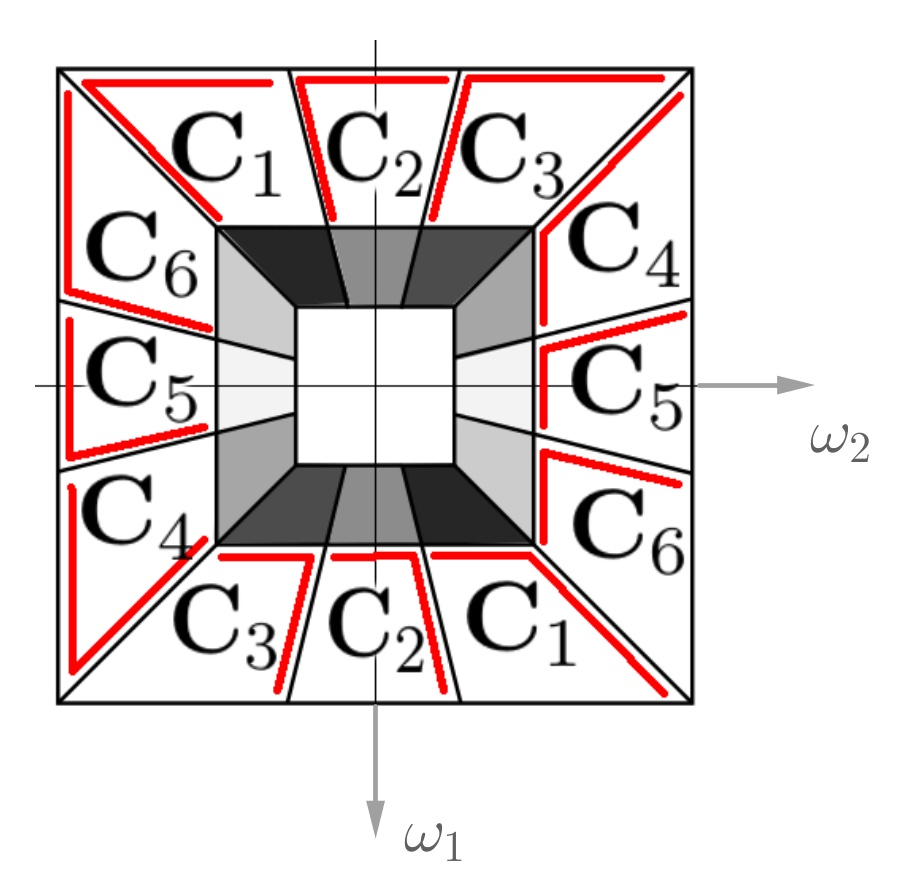
\includegraphics[width=\textwidth]{shannon-marked-wcoord.jpg}
\end{minipage}\hspace*{3em}
\begin{minipage}[c]{.3\textwidth}
\includegraphics[width=\textwidth]{sublattice-2.jpg}
\vspace*{1em}
\end{minipage}
\caption{Left: partition of $S_0$ and boundary assignment of $C_j$, $j = 1,\cdots,6$ ( each $C_j$ has boundaries indicated by red line segments), Right: dilated quincunx sub-lattice. }
\label{fig: partition}
\vspace*{-5mm}
\end{figure}

%\begin{mydef}
%If $\mathcal{L}$ is the lattice generated by $\boldsymbol{a}_1,\boldsymbol{a}_2$, i.e. $\mathcal{L} = \sum_{i=1,2}k_i\boldsymbol{a}_i,\,k_i\in\mathbb{Z}$,the {\bf reciprocal lattice} $\mathcal{L}^*$ of $\mathcal{L}$ is the lattice generated by the vectors $\boldsymbol{b}_1,\boldsymbol{b}_2$, s.t. $\boldsymbol{b}_i^T\boldsymbol{a}_j = 2\pi\delta_{ij}$. 
%\end{mydef}

%\begin{mydef}
%Given a lattice $\mathcal{L}$, a {\bf fundamental domain} $S$ in $\mathbb{R}^2$ with respect to $\mathcal{L}$, denoted as $S = \mathbb{R}^2/\mathcal{L}$, is a subset of $\mathbb{R}^2$, such that $\bigcup_{l\in\mathcal{L}}(S+l) = \mathbb{R}^2$ and $S\cap(S+l)=\varnothing,\,\forall l\in\mathcal{L}\setminus\{\mathbf{0}\}$.
%A set $S$ is a {\bf frequency support} of $\mathcal{L}$ if $S = \mathbb{R}^2/\mathcal{L}^*$.
%\end{mydef}
%Furthermore, each sub-lattice $\mathcal{L}$ of $\mathbb{Z}^2$ is associated with a set of shifts $\Gamma, \, s.t. \bigcup_{\V{\gamma}\in\Gamma}\mathcal{L}+\V{\gamma} = \mathbb{Z}^2$ and $|\Gamma| = |\mathbb{Z}^2/\mathcal{L}|$.

Consider the canonical frequency square, $S_0 = [-\pi,\pi)\times[-\pi,\pi)$ associated with lattice $\mathcal{L} = \mathbb{Z}^2$. 
%Due to \eqref{eq: m0} and \eqref{eq: mj}, this is equivalent to $S_0=\bigcup_{0\leq j\leq J} supp(m_j\vert_{S_0})$.That is, 
Consider a 1-level decomposition, \eqref{eq: MRA} together with \eqref{eq: m0} and \eqref{eq: mj} implies that the union of the support of $m_j,\,0\leq j\leq J$ covers $S_0$.
Furthermore, $\exists\, C_j\subset supp(m_j), 0\leq j\leq J,$ such that they form a partition of $S_0$, and it is natural to take $C_j$ as the main support of $m_j$.
To build an orthonormal basis with good directional selectivity, we choose the partition of $S_0$ shown in the left of Fig.\ref{fig: partition}, which is the same for Example B in \cite{durand2007} and the least redundant shearlet system. In this partition, $S_0$ is divided into a central square $C_0 = \bigl(\begin{smallmatrix} 2&0\\0&2\end{smallmatrix}\bigr)^{-1}S_0$ and a ring: the ring is further cut into six pairs of directional trapezoids $C_j$'s by lines passing through the origin with slopes $\pm 1, \pm 3$ and $\pm \frac{1}{3}$. The central square $C_0$ can be further partitioned in the same way to obtain a two-level multi-resolution system, as shown in Fig.\ref{fig: partition}. 


%To build our first example, in which $\hat{\phi},\,\widehat{\psi}^j$ are indicator functions in $\mathbb{R}^2$, we consider the case where  and we pick $S_0=\mathbb{R}^2/(\mathbb{Z}^2)^*$, . 
%Since $\phi_1,\psi^j_1$ and their shifts span the space $V_0$, $supp(\widehat{\phi}_1)$ and $supp(\widehat{\psi}^j)$, together, should thus cover $S_0$. Due to \eqref{eq: m0} and \eqref{eq: mj}, this is equivalent to $S_0=\bigcup_{0\leq j\leq J} supp(m_j\vert_{S_0})$. That is, if $C_j,\,{\small 0\leq j\leq J}$ are the main support of $m_j,\,0\leq j\leq J$ respectively, then they form a partition of $S_0$. An non-uniform admissible partition is defined as follows,

%\begin{mydef}
%$C_j, 0\leq j\leq J$ is an {\bf admissible} partition of $S_0$ if and only if $\exists \mathbf{D}, \mathbf{Q}\in\mathbb{Z}^{2\times 2}$, s.t. the low frequency piece $C_0 = \mathbb{R}^2/(\mathbf{D}\mathbb{Z}^2)^*,$ and the high frequency pieces $C_j = \mathbb{R}^2/(\mathbf{QD}\mathbb{Z}^2)^*,\,j = 1,\cdots,J$.
%\end{mydef}
Here $J= 6$ and $ |\mathbf{D}|^{-1} + J|\mathbf{QD}|^{-1} = 1/4 + 6/ (2\cdot 4) = 1$, hence the corresponding MRA generated by \eqref{eq: MRA} achieves critical downsampling(\cite{durand2007}). 
In addition, let {\small $\V{\pi}_0 = (0,0), \V{\pi}_1 = (\pi/2,\pi/2), \V{\pi}_2 = (\pi,0),\V{\pi}_3 = (-\pi/2,\pi/2), \V{\pi}_4 = (0,\pi), \V{\pi}_5 = (\pi/2,-\pi/2),\V{\pi}_6 = (\pi,\pi), \V{\pi}_7=(-\pi/2,-\pi/2)$}, then each piece $C_j$ together with its shifts form a tiling of $S_0$, i.e.
\begin{align}\label{eq: tiling}
S_0 = \bigcup_{\V{\pi}\in\Gamma_0}\left(C_j + \V{\pi}\right) = \bigcup_{\V{\pi}\in\Gamma_1}\left(C_0 + \V{\pi}\right),\quad j = 1,\cdots,6
%\mathbb{R}^2/(\mathbb{Z}^2)^*=\bigcup_{\V{\pi}\in\Gamma_0}\left(\mathbb{R}^2/(\V{D_2}\mathbb{Z}^2)^* %+ \V{\pi}\right)
%=\bigcup_{\V{\pi}'\in\Gamma_1}\left(\mathbb{R}^2/(\V{QD_2}\mathbb{Z}^2)^* + \V{\pi}'\right),
\end{align}
where
%then $\mathbf{D_2}\mathbb{Z}^2$ is associated with the set of shifts 
$\Gamma_0= \{\V{\pi}_i,\, i = 0,2,4,6\}$ and 
%$\mathbf{QD_2}\mathbb{Z}^2$ is associated with 
$\Gamma_1 = \{\V{\pi}_i,\, i = 0,1,\cdots,7\}$.
Alternatively, we say that $\{\,C_j,\, j = 0,\cdots,J\,\}$ is an {\it admissible} partition of $S_0$.
%This partition is admissible and corresponds to $\mathbf{D} = \mathbf{D_2}\doteq\bigl(\begin{smallmatrix} 2&0\\0&2\end{smallmatrix}\bigr)$ and $\mathbf{Q}:=\bigl(\begin{smallmatrix} 1&1\\-1&1\end{smallmatrix}\bigr)$. The wavelet coefficients are taken on the dilated quincunx sub-lattice $\mathbf{QD_2}\mathbb{Z}^2$ (see the right panel in Fig.\ref{fig: partition}).
%In addition, $|\mathbf{D_2}| = 4,\,|\mathbf{Q}| = 2$ so that $1/4 + 6/ (2\cdot 4) = 1$, and the system is critical downsampling.

\section{Orthonormal Bases}\label{sec: orth}

In this section, we discuss the conditions on $m_j$ such that the corresponding MRA forms an orthonormal bases. 
%consider orthonormal bases with $m-$functions defined in \eqref{eq: m0} and \eqref{eq: mj} whose supports mainly corresponding to the partition of $S_0$ in Fig.\ref{fig: partition}.
%we always consider a multi-resolution system with scaling function $\phi$ and quasi-shearlets $\psi^j$, {\small$ j = 1,\dots,6$} defined by $(M_0, D_2)$ and $(M_j, Q)$, {\small$j = 1,\dots,6$} respectively. Furthermore, the essential support of $M_j$'s corresponds to the partition of $\mathbf{S}_0$ in a shearlet system.

%The construction of \eqref{eq: MRA} reduces to design $m_0$ in \eqref{eq: m0} and $m_j, j= 1,\cdots,6$ in \eqref{eq: mj}.
We begin with the two key conditions, i.e. {\it identity summation} and {\it shift cancellation}, on $m_j$ such that the system \eqref{eq: MRA} is perfect-reconstruction (PR) or equivalently a Parseval frame in MRA.% weaker than the orthonormal condition.

%\subsection{Identity summation and shift cancellation}
\subsection{orthonormal conditions on $m_j$}\label{subsec: northonormal cond}
In MRA, \eqref{eq: MRA} is PR if $\forall f\in L_2(\mathbb{R}^2)$,
\begin{equation}
%\textstyle 
\sum_{\V{k}\in\mathbb{Z}^2}\langle f,\phi_{0,\V{k}}\rangle\phi_{0,\V{k}} = \sum_{\V{k}\in\mathbb{Z}^2}\langle f,\phi_{1,\V{k}}\rangle\phi_{1,\V{k}} + \sum_{j=1}^J\sum_{\V{k}'\in\V{Q}\mathbb{Z}^2}\langle f,\psi^{j}_{1,\V{k}'}\rangle\psi^j_{1,\V{k}'}.\label{eq: PR}
\end{equation}
Using \eqref{eq: m0} and \eqref{eq: mj} together with the admissibility of the frequency partition \eqref{eq: tiling}, condition \eqref{eq: PR} on $\phi$ and $\psi^j$ yields:
\begin{thm}\label{thm: conds}
Let $J=6,\, \V{D} =\bigl(\begin{smallmatrix} 2&0\\0&2\end{smallmatrix}\bigr)$ and $\V{Q}\doteq\bigl(\begin{smallmatrix} 1&1\\-1&1\end{smallmatrix}\bigr)$ in \eqref{eq: MRA}.
Then the perfect reconstruction condition holds for \eqref{eq: MRA} iff the following two conditions hold
\begin{align}\label{eq: id-sum}
|m_0(\boldsymbol{\omega})|^2 + \sum_{j = 1}^6|m_j(\boldsymbol{\omega})|^2 = 1
\end{align}
\begin{equation}\label{eq: shift-cancel}
 \begin{cases}
%M_0(\boldsymbol{omega})\overline{M_0(\boldsymbol{omega}+\boldsymbol{\gamma})} + 
\sum_{j = 0}^6m_j(\boldsymbol{\omega})\overlinespace{m_j}(\boldsymbol{\omega} + \boldsymbol{\pi}) = 0, & \boldsymbol{\pi}\in \Gamma_0\setminus\{\boldsymbol{0}\}\\[.5em]
\sum_{j=1}^6m_j(\boldsymbol{\omega})\overlinespace{m_j}(\boldsymbol{\omega}+\boldsymbol{\pi}) = 0, & \boldsymbol{\pi}\in\Gamma_1\setminus\Gamma_0
\end{cases}
\end{equation}
%where  $\Lambda = (QD\mathbb{Z}^2)^*/(\mathbb{Z}^2)^*,\,\Gamma = (D\mathbb{Z}^2)^*/(\mathbb{Z}^2)^*.$ %$\{(\frac{\pi}{2},\frac{\pi}{2}),(\frac{3\pi}{2},\frac{\pi}{2}),(\frac{\pi}{2},\frac{3\pi}{2}),(\frac{3\pi}{2},\frac{3\pi}{2}),$ $(0,0),(0,\pi),(\pi,0),(\pi,\pi)\}$
\end{thm}

Theorem \ref{thm: conds} is a corollary of Prop. 1 and Prop. 2 in \cite{durand2007}. We give an alternate proof in Appendix \ref{app: cond-thm}.
In Theorem \ref{thm: conds}, Eq. \eqref{eq: id-sum} is the {\it identity summation} condition, guaranteeing conservation of $l_2$ energy; Eq. \eqref{eq: shift-cancel} is the {\it shift cancellation} condition such that aliasing is canceled correctly in reconstruction from wavelet coefficients. %, such that downsampling of scaling and shearlet coefficients is valid. 
 %$\Lambda = \{(\frac{\pi}{2},\frac{\pi}{2}),(\frac{3\pi}{2},\frac{\pi}{2}),(\frac{\pi}{2},\frac{3\pi}{2}),(\frac{3\pi}{2},\frac{3\pi}{2}),$ $(0,0),(0,\pi),(\pi,0),(\pi,\pi)\},\Gamma = \{(0,0),(0,\pi),(\pi,0),(\pi,\pi)\}$ are the sets of shifts associated to quincunx-dyadic dilation $QD$ and dyadic dilation $D$ respectively.
%Each $M_j$ contributes a term $M_j(\boldsymbol{omega})\overline{M_j(\boldsymbol{omega} + \boldsymbol{\nu})}$ in the cancellation condition of any shift $\boldsymbol{\nu}$ corresponding to the downsampling scheme of $M_j$.
Because each $m_j$ is $(2\pi,2\pi)$ periodic, we only need to check these conditions $\forall \V{\omega}\in S_0$.

%\subsection{Extra condition for basis}
%By Theorem \ref{thm: conds}, the system \eqref{eq: MRA} is a Parseval frame ; 
Moreover, for  \eqref{eq: MRA} to be an orthonormal basis,  $\{\phi_{\boldsymbol{k}}\}_{\boldsymbol{k}\in\mathbb{Z}^2}$ need to be an orthonormal basis, which is determined by $m_0$ in \eqref{eq: phi-m0}. In 1D MRA, Cohen's theorem in \cite{cohen1992biorthogonal} provides a necessary and sufficient condition on $m_0$ such that \eqref{eq: MRA} is an orthonormal basis. %Such a condition in 1D wavelet MRA is given by Cohen \cite{cohen1992biorthogonal}. 
This theorem generalizes to 2D as proved in  e.g. \cite{yin2014orthshear}, as follows.
\begin{thm}\label{thm: basis cond}
Assume that $m_0$ is a trigonometric polynomial with $m_0(\V{0})=1$, and define $\hat{\phi}(\boldsymbol{\omega})$ as in \eqref{eq: phi-m0}.\\
If $\phi(\cdot - \boldsymbol{k}),\boldsymbol{k}\in\mathbb{Z}^2$ are orthonormal, then $\exists K$ containing a neighborhood of 0, s.t. $\forall\boldsymbol{\omega}\in S_0,\,\boldsymbol{\omega}+2\pi\mathbf{n}\in K$ for some $\mathbf{n}\in\mathbb{Z}^2, $ and $\inf_{k>0,\,\boldsymbol{\omega}\in K}|m_0(\mathbf{D_2}^{-k}\boldsymbol{\omega})| >0$. 
 Further, if $\sum_{\boldsymbol{\V{\pi}}\in \Gamma_0} |m_0(\boldsymbol{\omega}+\boldsymbol{\pi})|^2 = 1$, then the inverse is true.
\end{thm}
%Theorem \ref{thm: basis cond} can be proved similarly to Cohen's theorem (\cite{cohen1992biorthogonal}).
%Because it is difficult to directly design $M_0$ that satisfies the conditions in Theorem \ref{thm: basis cond}, 
%Below, we construct $m-$functions imposing only \eqref{eq: id-sum} and \eqref{eq: shift-cancel} and then check if the resulting Parseval frame is an orthonormal basis by applying Theorem \ref{thm: basis cond} to $m_0$.

\subsection{Regularity of $m_j$ supported on the $C_j$}\label{sec: design}
%In this section, we define Shannon-type directional orthonormal basis same as in \cite{durand2007} and \cite{nuDFB05}. Then, we apply direct smoothing to its $m-$functions to improve spatial localization, this leads to a critical analysis of the boundary regularity of $S_1$ and the $C_j$'s.

%\subsection{Shannon-type wavelets and smoothing}
In this subsection, we consider $m_j$ supported on the $C_j$ introduced in Section \ref{subsec: frequency partition} that satisfy orthonormal conditions in Section \ref{subsec: northonormal cond}. We begin with the Shannon-type wavelet construction,
where $m_j$ are indicator functions $ m_j = \mathbbm{1}_{C_j},\,0\leq j \leq 6,\,$ and we use the boundary assignment of $C_j$ in Fig.\ref{fig: partition}.
The identity summation follows from the partition of $S_0$ by the $C_j$, and the shift cancellation follows from the tiling property \eqref{eq: tiling}. % which implies $m_j(\boldsymbol{\omega})\overline{m_j(\boldsymbol{\omega} + \boldsymbol{\pi}_i)}\equiv 0,\,\forall j,\, i\neq 0.$ %Let $\partial\mathbf{C}_j = \overline{\mathbf{C}_j}-\mathbf{C}_j^{\circ}$ be the boundary of $\mathbf{C}_j$,  
Applying Theorem \ref{thm: basis cond} to $m_0$, we verify that the Shannon-type wavelets generated from these $m_j$ form an orthonormal basis.

%However, because of the discontinuity of $m_j$ across the boundary of its support, the corresponding wavelet has slow decay in the time domain. 
%Such $m_j$'s are not regularized due to 
Because of the discontinuity at $\partial C_j$, the boundaries of the $C_j$, these $m_j$ are not smooth, and hence the corresponding wavelets are not spatially localized. The $m_j$ can be regularized by smoothing at the $\partial C_j$.
%We take a different regularization approach from Durand's \cite{durand2007}, where three regular quincunx filter banks are constructed and then composed to obtain the desired regular quincunx dyadic filter banks. Here, we smooth the discontinuous boundaries of $m-$functions directly. 
However, as shown in Proposition 3 in \cite{durand2007}, it is not possible to smooth the behavior of the $m_j$ at  {\it all} the boundaries with discontinuity if the $m_j$ have to satisfy the perfect reconstruction condition.
In \cite{yin2014orthshear}, the $\partial C_j$ are segmented into {\it singular} and {\it regular} pieces. On regular boundaries, pairs of $(m_j,\, m_{j'})$ share a boundary and can both be smoothed in a coherent way such that all the constraints in Theorem \ref{thm: basis cond} remain satisfied. The singular pieces are boundaries for just one $m_j$, which can then not be smoothed without violating the shift cancellation condition. Fig. \ref{fig: boundary} shows the boundary classification, where the corners of $S_0$ and $C_0$ are singular, hence $m_0$ and the $m_j$'s in two diagonal directions of an orthonormal bases are discontinuous there. A mechanism of constructing orthonormal bases by smoothing Shannon-type $m_j$ on regular boundaries is provided in \cite{yin2014orthshear}.%However, it remains unclear if some of the discontinuity can be removed by direct smoothing.

%Next, we analyze the limitation of direct smoothing in detail and show that there are regular boundaries which can be smoothed without violating \eqref{eq: id-sum} and \eqref{eq: shift-cancel}, and singular boundaries which cannot be smoothed.

%\textcolor{red}{In the remainder of this paper, we explore how this can be done for the first dyadic layer (without cutting further at higher frequencies); we call the corresponding basis {\it quasi-Shearlets}.}

\begin{figure}[!t]
\centering
%\hspace*{-5mm}
%\begin{minipage}{.6\textwidth}
%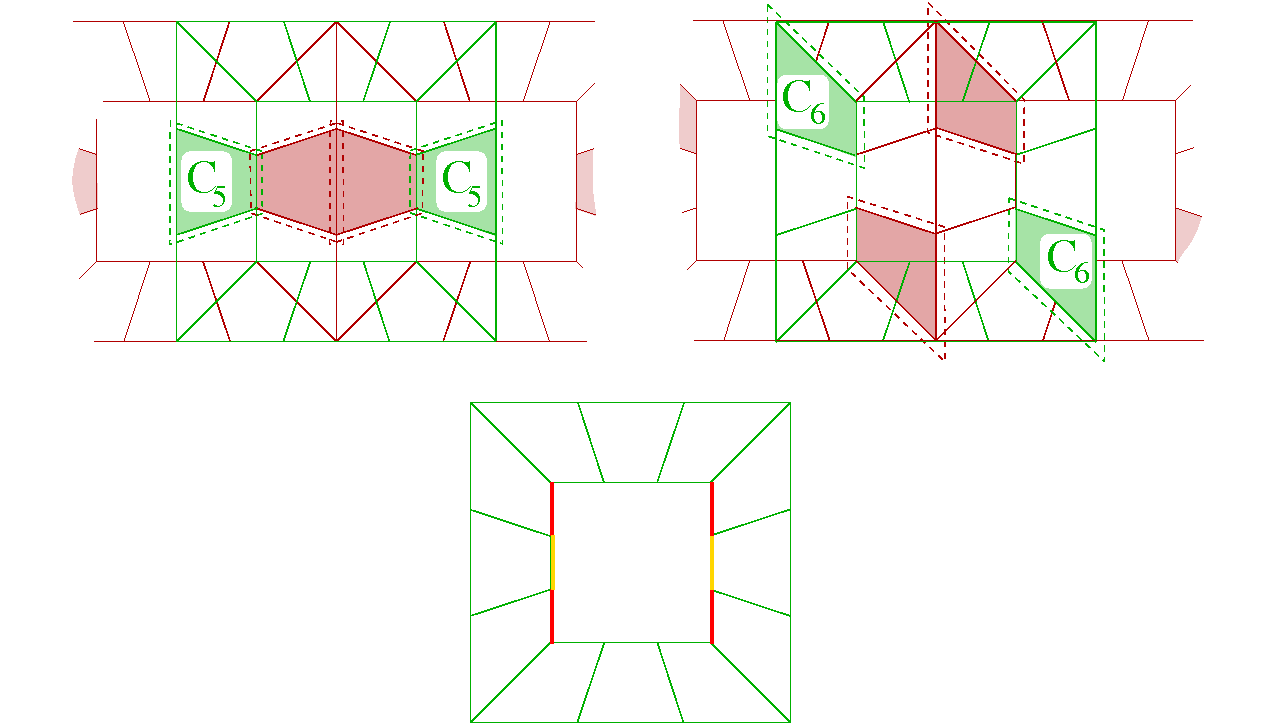
\includegraphics[width=\textwidth]{fig_overlap.png}\hspace*{-2mm}
%\end{minipage}
\begin{minipage}{.3\textwidth}
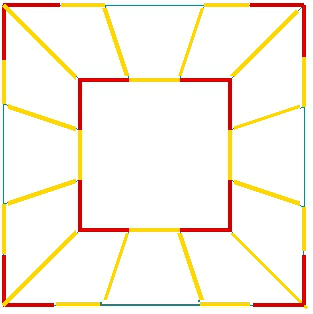
\includegraphics[width=\textwidth]{bdyclass.jpg}
\end{minipage}
%\includegraphics[width=.2\textwidth]{fig/sublattice-2.jpg}
\caption[caption]{
%\textcolor{red}{
%{\it Left top}: the supports of $m_j$ (green) and $m_j(\cdot+\V{\pi}_2$ (red) for $j = 5,6$ after smoothing, overlap on the vertical boundary at $\omega_1 =  \pm \pi/2$ of $C_5$ (green) and its shift (red) by $\boldsymbol{\pi}_2 = (\pi,0)$. Note that two copies of shifted $S_0$ (red) overlap the un-shifted $S_0$(green) due to the $(2\pi,2\pi)$ periodicity of $m_j$. Only $m_0$ and $m_5$ have overlapping smoothed boundaries by $\boldsymbol{\pi}_2$. 
%\\\hspace{\textwidth}
%{\it Left bottom}: intersection of $\mathcal{B}(0,\boldsymbol{\pi}_2)$ and $\mathcal{B}(5,\boldsymbol{\pi}_2)$ in yellow and $\mathcal{C}(0,\boldsymbol{\pi}_2) = \mathcal{B}(0,\boldsymbol{\pi}_2)\setminus\mathcal{B}(5,\boldsymbol{\pi}_2)$ in red. Smoothing $m_0$ in the red (singular) region is impossible without violating \eqref{eq: shift-cancel}. %This leads to the distinction between regular (yellow) and singular (red) boundaries at $omega_1 = \pm\pi/2$.
%\\\hspace{\textwidth}
%{\it Right}: 
Boundary classification, singular (red) and regular (yellow) }%after similar arguments for all shifts $\boldsymbol{\pi}_i$.}
 %}
\label{fig: boundary}
\end{figure}

\begin{comment}
%\subsection{Boundary classification}
 After smoothing the $m_j$'s, the shift cancellation \eqref{eq: shift-cancel} may fail to hold as $supp(m_j)$ and $(supp(m_j)-\boldsymbol{\pi})$ may overlap near the smoothed boundaries, see Fig. \ref{fig: boundary}, illustrating $m_5(\boldsymbol{\omega})\overline{m_5(\boldsymbol{\omega} + \boldsymbol{\pi}_2)}\not\equiv 0.$
For simplicity, we introduce the following notations: let 
$\mathcal{B}(j,\boldsymbol{\pi}) =  supp(m_j)\cap\,(supp(m_j)-\boldsymbol{\pi})$ be the support of  $m_j(\boldsymbol{\omega})\overline{m_j(\boldsymbol{\omega} + \boldsymbol{\pi})}$ associated to $m_j$ and shift $\boldsymbol{\pi}$;
let $\mathcal{C}(j,\boldsymbol{\pi}) = \mathcal{B}(j,\boldsymbol{\pi}) \setminus \bigcup_{j'\neq j}\mathcal{B}(j',\boldsymbol{\pi})$. 
%In addition, we may introduce the (slight abuse of) notation $C_0 = S_1$.
\begin{lem}\label{lem: singular-bdy}
Shift cancellation \eqref{eq: shift-cancel} can hold for shift $\boldsymbol{\pi}\in\Gamma_0\setminus\{\boldsymbol{0}\}$, only if $\mathcal{C}(j,\boldsymbol{\pi})=\varnothing,\, \forall\, 0\leq j\leq 6$; 
it can hold for shift $\boldsymbol{\pi}\in\Gamma_1\setminus\Gamma_0$, only if $\mathcal{C}(j,\boldsymbol{\pi})=\varnothing,\, \forall\, 1\leq j\leq 6$. 
\end{lem}
\noindent{\it Proof.} Observe that, on $\mathcal{C}(j,\boldsymbol{\pi})$, $m_j(\boldsymbol{\omega})\overline{m_{j}(\boldsymbol{\omega}+\boldsymbol{\pi})} \not\equiv 0$ but $m_{j'}(\boldsymbol{\omega})\overline{m_{j'}(\boldsymbol{\omega}+\boldsymbol{\pi})} \equiv 0,\, \forall j' \neq j$, hence \eqref{eq: shift-cancel} doesn't hold. $\hfill\square$
%Furthermore, the identity summation constraint \eqref{eq: id-sum} implies that $|M_j(\boldsymbol{omega})| = 1$ on $\mathcal{C}(j,\boldsymbol{\nu}),\,\forall\boldsymbol{\nu}$, hence the discontinuity of $M$-functions across these boundaries is unavoidable.
 
Therefore, boundaries that after smoothing make $\mathcal{C}(j,\boldsymbol{\pi})$ non-empty are called {\it singular}; the rest are {\it regular}. We next provide an explicit boundary classification method:
\begin{prop}\label{prop: class-bdy}
$\forall\, 1\leq j\leq 6$, let $supp(m_j) = \ov{$C_j$}$, then the boundary of $C_j$ is $\partial C_j=\bigcup_{i \neq 0}\mathcal{B}(j,\boldsymbol{\pi}_i)$. The set of singular boundaries of $\partial C_j$ is $\bigcup_{i\neq 0}\mathcal{C}(j,\boldsymbol{\pi}_i)$, whereas its compliment set is the regular boundary set.
 \end{prop}
\noindent{\it Proof.} Since $\bigcup_i(C_j+\boldsymbol{\pi}_i) = S_0$, $\partial C_j\subset \bigcup_{i\neq 0} (\ov{$C_j$}+\boldsymbol{\pi}_i) $. Therefore, $\partial C_j\subset\bigcup_{i\neq 0}\mathcal{B}(j,\boldsymbol{\pi}_i)$. On the other hand, $\mathcal{B}(j,\boldsymbol{\pi}_i)\subset \partial\mathbf{C}_j, \forall \, i\neq 0$, hence the union of them is a subset of $\partial C_j$. It follows that $\mathcal{B}(j,\boldsymbol{\pi}_i)$ form a partition of the boundary $\partial C_j$. The partition of $\partial C_j$ into singular and regular boundaries follows from Lemma \ref{lem: singular-bdy}.$\hfill\square$

 The case of $\partial S_1$ is similar where $\mathcal{B}(0,\boldsymbol{\pi}),\,\boldsymbol{\pi}\in\Gamma_0\setminus\{0\}$ are considered. We use the notation $\mathcal{B}_s(j,\boldsymbol{\pi}),\mathcal{C}_s(j,\boldsymbol{\pi})$ for the special case $supp(m_j) = \ov{$C_j$}$ hereafter.
The boundary classification based on Proposition \ref{prop: class-bdy} is shown in the right of Fig. \ref{fig: boundary}, where the boundaries on the four corners of both $S_0$ and $S_1$ are singular: smoothing is then not allowed there.

\begin{prop}\label{prop: jump}
Let $\mathcal{C} = \mathcal{C}_s(j_1,\boldsymbol{\pi}_{i_1})\cap \mathcal{C}_s(j_2,\boldsymbol{\pi}_{i_2})$, if $m_{j_1}, m_{j_2}$ satisfy \eqref{eq: id-sum}, \eqref{eq: shift-cancel}, then $|m_{j_1}|=\mathbbm{1}_{\mathbf{C}_{j_1}},\,|m_{j_2}|=\mathbbm{1}_{\mathbf{C}_{j_2}}$ on $\mathcal{C}$.
\end{prop}
\noindent{\it Proof.} Suppose the common singular boundary $\mathcal{C}$ is non-empty and observe that $\mathcal{C}\subset(C_{j_1})\cap(C_{j_2})$. Since $m_{j_1}$ cannot be smoothed on $\mathcal{C}_s(j_1,\boldsymbol{\pi}_{i_1})$, $|m_{j_1}| = 0$ on $\mathcal{C}_s(j_1,\boldsymbol{\pi}_{i_1})\setminus\mathbf{C}_{j_1}$, 
%Because $\mathcal{C}\subset\mathcal{C}_s(j_1,\boldsymbol{\nu}_1)\cap\partial\mathbf{C}_{j_2}$, 
and \eqref{eq: id-sum} implies that $|m_{j_2}| = 1$ there, or equivalently $|m_{j_2}|=\mathbbm{1}_{\mathbf{C}_{j_2}}$ on $\mathcal{C}$. Similarly, $|m_{j_1}|=\mathbbm{1}_{\mathbf{C}_{j_1}}$ on $\mathcal{C}.\hfill\square$

Prop. \ref{prop: jump} shows that if $m_j$ and $m_{j'}$ have common singular boundaries, then both will have a discontinuity across those boundaries. For example, $\mathcal{C}_s(0,(\pi,0))\cap\mathcal{C}_s(4,(\pi/2,\pi/2)) = (\pi/2,(\pi/6,\pi/2))$, hence $m_0$ and $m_4$ both are discontinuous at $(\pi/2,(\pi/6,\pi/2))$. All the singular boundaries related to \eqref{eq: MRA} are such "double" singular boundaries.

\subsection{Pairwise smoothing of regular boundary}
%Despite of the singular boundaries, better spatial localization can be achieved by carefully smoothing the regular boundaries. 
The regular boundaries of both $C_{j_1}$ and $C_{j_2}$ with adjacent supports consist of $\mathcal{B}_s(j_1,\boldsymbol{\pi})\cap\mathcal{B}_s(j_2,\boldsymbol{\pi})$, which we denote by the triple $(j_1,j_2,\boldsymbol{\pi})$. The following proposition shows that the regular boundaries $(j_1,j_2,\boldsymbol{\pi})$ can be paired according to shift pairs $(\boldsymbol{\pi},-\boldsymbol{\pi})$, and the boundaries must be smoothed pairwise within their $\epsilon-$neighborhood, $\mathcal{B}_{\epsilon}(j_1,j_2,\boldsymbol{\pi})$ and $\mathcal{B}_{\epsilon}(j_1,j_2,-\boldsymbol{\pi})$.

\begin{prop}\label{prop: pair-smooth}
Given $(j_1,j_2,\boldsymbol{\pi})\neq \varnothing$, %let $\boldsymbol{\nu}'= -\boldsymbol{\nu}\in \mathbb{R}^2/(\mathbb{Z}^2)^*$, 
then $(j_1,j_2,-\boldsymbol{\pi})\neq\varnothing$. In addition, let $\mathcal{B}=\mathcal{B}_{\epsilon}(j_1,j_2,\boldsymbol{\pi})\cup\mathcal{B}_{\epsilon}(j_1,j_2,-\boldsymbol{\pi})$. Then the identity summation and shift cancellation conditions hold if
\begin{itemize}
\item[{\it (i)}] $m_j = \mathbbm{1}_{C_j},\quad\text{on }S_0,\; j\neq j_1,j_2$
\item[{\it (ii)}] $m_{j_1} =\mathbbm{1}_{C_{j_1}},\, m_{j_2} =\mathbbm{1}_{C_{j_2}},\quad \text{on }\mathcal{B}^c$\\[.5em]
\hspace*{-2em} and on $\mathcal{B}$ the following hold%\vspace*{.1em}
\item[{\it(iii)}] $|m_{j_1}|^2 + |m_{j_2}|^2 = 1,$ %\hfill on $ \mathcal{B}_{\epsilon}(j_1,j_2,\nu)\cup\mathcal{B}_{\epsilon}(j_1,j_2,\nu')$
\item[{\it (iv)}] $\sum_{j_1,j_2} m_j(\cdot)\overline{m_j(\cdot+\widetilde{\boldsymbol{\pi}})} = 0,\, \widetilde{\boldsymbol{\pi}} = \pm\boldsymbol{\pi}$
%\hspace*{8em} on $\mathcal{B}_{\epsilon}(j_1,j_2,\nu)$ and $\mathcal{B}_{\epsilon}(j_1,j_2,\nu)-\nu$
%\item[{\it (v)}] $\sum_{j_1,j_2} M_j(\cdot)\overline{M_j(\cdot+\boldsymbol{\nu}')} = 0.$ 
%\hspace*{7em} on $\mathcal{B}_{\epsilon}(j_1,j_2,\boldsymbol{\nu}')$ and $\mathcal{B}_{\epsilon}(j_1,j_2,\nu')-\nu'$
\end{itemize}
\end{prop}
\noindent{\it Proof}.
 We first show that $(j_1,j_2,-\boldsymbol{\pi})\neq\varnothing.$ By definition, $\mathcal{B}_s(j_1,\boldsymbol{\pi}) = supp(m_{j_1})\cap (supp(m_{j_1})-\boldsymbol{\pi}) = \left((supp(m_{j_1})+\boldsymbol{\pi})\cap supp(m_{j_1})\right)-\boldsymbol{\pi} = \mathcal{B}_s(j_1,-\boldsymbol{\pi})-\boldsymbol{\pi}.$ Rewrite $(j_1,j_2,\boldsymbol{\pi})$ by $\mathcal{B}_s(j_1,-\boldsymbol{\pi})$ and $\mathcal{B}_s(j_2,-\boldsymbol{\pi})$, we have $(j_1,j_2,-\boldsymbol{\pi}) = (j_1,j_2,\boldsymbol{\pi})+\boldsymbol{\pi}$, hence it's non-empty.
 
Because $(j_1,j_2,\pm\boldsymbol{\pi})\subset (\partial C_{j_1} \bigcap \partial C_{j_2})$ and $(\bigcup_{j}C_j)=S_0$, $(\bigcup_{j\neq j_1,j_2}C_j)\cap \mathcal{B} = \varnothing.$ Therefore, smoothing of $m_{j_1}$ and $m_{j_2}$ in $\mathcal{B}$ doesn't impact the region where other $m_j$'s are supported.

We then show that the cancellation conditions \eqref{eq: shift-cancel} hold for all shifts. Condition (i) and (ii) imply that $\mathcal{B}(j,\widetilde{\boldsymbol{\pi}})= \varnothing,\,\forall j,\widetilde{\boldsymbol{\pi}}\neq \pm \boldsymbol{\pi}$, hence \eqref{eq: shift-cancel} hold for $\widetilde{\boldsymbol{\pi}}\neq \pm \boldsymbol{\pi}$. %For $\boldsymbol{\nu}$, 
(i) implies $\mathcal{B}(j,\widetilde{\boldsymbol{\pi}}) = \varnothing,\,\forall j\neq j_1,j_2$, so then \eqref{eq: shift-cancel} is equivalent to (iv). %Similarly, \eqref{eq: shift-cancel} is equivalent to (v) under (i).
The identity summation \eqref{eq: id-sum} holds due to (i), (ii) and (iii).$\hfill\square$.

By Prop. \ref{prop: pair-smooth} we can smooth some pairs of regular boundaries starting from the Shannon-type directional wavelets with the simplified conditions (iii), (iv) and (v); (i) and (ii) can be removed as long as the initial $m_j$ satisfy \eqref{eq: id-sum} and \eqref{eq: shift-cancel} and every $\boldsymbol{\omega}\in S_0$ is not covered by more than two $m$ functions. We can thus smooth regular boundaries pairwise, one by one.

The next proposition gives an explicit design of $(m_{j_1}, m_{j_2})$ satisfying the simplified conditions (iii),(iv) in Proposition \ref{prop: pair-smooth}. %as well as a necessary condition for any valid design.
\begin{prop}\label{prop: m-design}
Let $C\subset S_0$, given $m_{j_1},m_{j_2}\neq 0$ continuous on $ C\cup(C+\boldsymbol{\pi})$, satisfying the following conditions
\begin{itemize}
\item[(i)] $\sum_{j_1,j_2}m_{j}(\boldsymbol{\omega})\overline{m_{j}(\boldsymbol{\omega}+\boldsymbol{\pi})} = 0$ \hspace*{2em} on $C$
\item[(ii)] $\sum_{j_1,j_2}|m_{j}(\boldsymbol{\omega})|^2= 1 $ \hspace*{5em} on $C\cup (C+\boldsymbol{\pi})$
\item[(iii)] $m_{j_1}(\boldsymbol{\omega})m_{j_2}(\boldsymbol{\omega}) = 0$\hspace*{5em} on $\partial C$ ;
\end{itemize}
then
$\quad|m_{j_1}(\boldsymbol{\omega})| = |m_{j_2}(\boldsymbol{\omega}+\boldsymbol{\pi})|,\quad |m_{j_2}(\boldsymbol{\omega})| = |m_{j_1}(\boldsymbol{\omega}+\boldsymbol{\pi})|.$\\[1mm]
Furthermore, if $m_{j} = e^{i\boldsymbol{\omega}^{T}\boldsymbol{\eta}_{j}}\mathrm{m}_{j},\quad j=j_1,j_2, \text{ on }C,$ where $\mathrm{m}_j$ is a real-valued function, % $\mathcal{M}_{j_1}$ and $\mathcal{M}_{j_2}$,  phase $\eta_1,\eta_2$ s.t.
$e^{i\boldsymbol{\pi}^T(\boldsymbol{\eta}_{j1}-\boldsymbol{\eta}_{j2})} = -1,$ and 
\[\mathrm{m}_{j_1}(\boldsymbol{\omega}) = \mathrm{m}_{j_2}(\boldsymbol{\omega}-\boldsymbol{\pi}),\;\mathrm{m}_{j_2}(\boldsymbol{\omega}) = \mathrm{m}_{j_1}(\boldsymbol{\omega}-\boldsymbol{\pi}),\text{ on }C+\boldsymbol{\pi},\] 
%where $\mathcal{M}_{j1},\,\mathcal{M}_{j2}$ are 
then $(i)$ holds.
\end{prop}
\noindent{\it Proof.} 
To prove the necessary condition, note that (i) implies $|m_{j_1}(\boldsymbol{\omega})|^2|m_{j_1}(\boldsymbol{\omega+\pi})|^2 = |m_{j_2}(\boldsymbol{\omega})|^2|m_{j_2}(\boldsymbol{\omega+\pi})|^2$; the condition then follows from (ii).
For the sufficient construction, check by directly substituting the construction into (i). $\hfill\square$
%For the necessary condition, we prove in two cases. Suppose $|M_{j_1}|  = |M_{j_2}|$ on $\omega$, then (ii) implies $|M_{j_1}| = |M_{j_2}| = \frac{1}{2}$ on $\omega$. From (i), it's necessary $|M_{j_1}(\boldsymbol{omega}+\boldsymbol{\nu})|=|M_{j_2}(\boldsymbol{omega}+\boldsymbol{\nu})|$ on $\omega$, or equivalently, $|M_{j_1}| = |M_{j_2}|$ on $\omega + \boldsymbol{\nu}$. Apply (ii) again, we have $|M_{j_1}| = |M_{j_2}| = \frac{1}{2}$ on $\omega+\boldsymbol{\nu}$, therefore, $|M_{j_1}(\boldsymbol{omega})| = |M_{j_2}(\boldsymbol{omega}+\boldsymbol{\nu})|=|M_{j_2}(\boldsymbol{omega})| = |M_{j_1}(\boldsymbol{omega}+\boldsymbol{\nu})|=\frac{1}{2}.$%However, (iii) implies that either $M_{j_1}$ or $M_{j_2}$ decays to zero on the boundary, therefore, $|M_{j_1}$ and $|M_{j_2}|$ cannot be constant.

%Suppose now $|M_{j_1}(\boldsymbol{omega})| = |M_{j_2}(\boldsymbol{omega}+\boldsymbol{\nu})|$ on $\omega$, then (i) implies $|M_{j_2}(\boldsymbol{omega})| = |M_{j_1}(\boldsymbol{omega}+\boldsymbol{\nu})|$ on $\omega$.


Proposition \ref{prop: m-design} breaks down the design of $(m_{j_1},m_{j_2})$ into a pair of real functions $(\mathrm{m}_{j_1}, \mathrm{m}_{j_2})$ on $\mathcal{B}_{\epsilon}(j_1,j_2,\boldsymbol{\pi})$ and two vectors $\boldsymbol{\eta}_1,\boldsymbol{\eta}_2$; then $(\mathrm{m}_{j_1}, \mathrm{m}_{j_2})$ on $\mathcal{B}_{\epsilon}(j_1,j_2,-\boldsymbol{\pi})$ are automatically determined. %When all regular boundaries adopt this smoothing scheme,  each $\mathcal{M}_j$ has to locally match up with every $\mathcal{M}_{j'}$'s that shares a regular boundary $(j,j',\nu)$. Therefore, we may focus on 
The only constraint on $(\mathrm{m}_{j_1},\mathrm{m}_{j_2})$ for (ii) in Proposition \ref{prop: m-design} to hold is that on $\mathcal{B}_{\epsilon}(j_1,j_2,\boldsymbol{\pi})$, $\sum_{j_1,j_2}|\mathrm{m}_{j}(\boldsymbol{\omega})|^2= 1$, which is easy to be satisfied.
We may construct all local pairs of $(\mathrm{m}_{j_1},\mathrm{m}_{j_2})$ separately, and put together afterwards different pieces of each $\mathrm{m}_j$ located in different regular boundary neighborhoods $\mathcal{B}_{\epsilon}(j,j',\boldsymbol{\pi})$. 

\vspace*{.2em}
%The phase term $e^{i\boldsymbol{omega}^T\boldsymbol{\eta}_j}$ is preferably defined on the full frequency domain, hence $\boldsymbol{\eta}_j$'s need to be solved globally. This global phase problem is stated precisely in t
The next proposition gives % conditions for the $\boldsymbol{\eta}_j$ as well as 
one solution, easy to verify.
\begin{prop}\label{prop: phase}
Applying Proposition \ref{prop: m-design} to all regular boundaries requires a set of phases $\{\boldsymbol{\eta}_j\}_{j = 0}^6,$ s.t.\[\textstyle e^{i\boldsymbol{\nu}^T(\boldsymbol{\eta}_{j1}-\boldsymbol{\eta}_{j2})} = -1, \quad\forall (j_1,j_2,\boldsymbol{\pi})\in\Delta,\]
{\small\begin{multline*}
\Delta = \Bigl\{\big(0,2,(0,\pi)\big),\, \big(0,5,(\pi,0)\big),\,\big(1,3,(\pi,0)\big),\,\big(4,6,(0,\pi)\big),\\
\big(1,6,(\pi/2, 3\pi/2)\big),\,\big(2,3,(\pi/2, 3\pi/2)\big),\,\big(4,5,(\pi/2, 3\pi/2)\big), \\
\big(3,4,(\pi/2, \pi/2)\big),\big(1,2,(\pi/2, \pi/2)\big),\,\big(5,6,(\pi/2, \pi/2)\big)\Bigr\}
\end{multline*}}
The following is a (non-unique) solution: 
{\small\begin{multline*}\boldsymbol{\eta}_0 = (0,0),\,\boldsymbol{\eta}_1 = (0,0),\,\boldsymbol{\eta}_2 = (1,1),\,\boldsymbol{\eta}_3 = (1,-1),\\
\boldsymbol{\eta}_4 = (0,2),\,\boldsymbol{\eta}_5=(1,1),\,\boldsymbol{\eta}_6 = (-1,1).
\end{multline*}}
\end{prop}

To summarize, Proposition \ref{prop: m-design} and \ref{prop: phase} introduce the following regular boundary smoothing scheme for the $m$ functions:
\begin{description}% prevent items from splitting
\item[construction of orthonormal basis]\
\begin{itemize}
\item[1.] First, set $\mathrm{m}_j = \mathbbm{1}_{C_j}$; then smoothen these across a pair of regular boundaries $(j_1,j_2,\pm\boldsymbol{\pi})$ following steps 2, 3.
\item[2.]  On $\mathcal{B}_{\epsilon}(j_1,j_2,\boldsymbol{\pi})$,\\
\hspace*{2em} design $(\mathrm{m}_{j_1},\mathrm{m}_{j_2}),\quad$ s.t.
$\sum_{j_1,j_2}|\mathrm{m}_{j}(\boldsymbol{\omega})|^2= 1$.
\item[3.] On $\mathcal{B}_{\epsilon}(j_1,j_2,-\boldsymbol{\pi})$, \\
\hspace*{2em}let $\mathrm{m}_{j_1}(\boldsymbol{\omega}) = \mathrm{m}_{j_2}(\boldsymbol{\omega}-\boldsymbol{\pi})$, $\mathrm{m}_{j_2}(\boldsymbol{\omega}) = \mathrm{m}_{j_1}(\boldsymbol{\omega}-\boldsymbol{\pi})$\vspace*{.1em}
\item[4.] Repeat step 2 and 3 for all $(j_1,j_2,\boldsymbol{\pi})\in\Delta$. 
\item[5.]$m_j(\boldsymbol{\omega}) =e^{i\boldsymbol{\omega}^T\boldsymbol{\eta}_j} \mathrm{m}_j(\boldsymbol{\omega}),$ on $S_0$, with the $\boldsymbol{\eta}_j$ of Prop. \ref{prop: phase}.
\end{itemize}
\end{description}

\begin{figure}[!t]
\centering
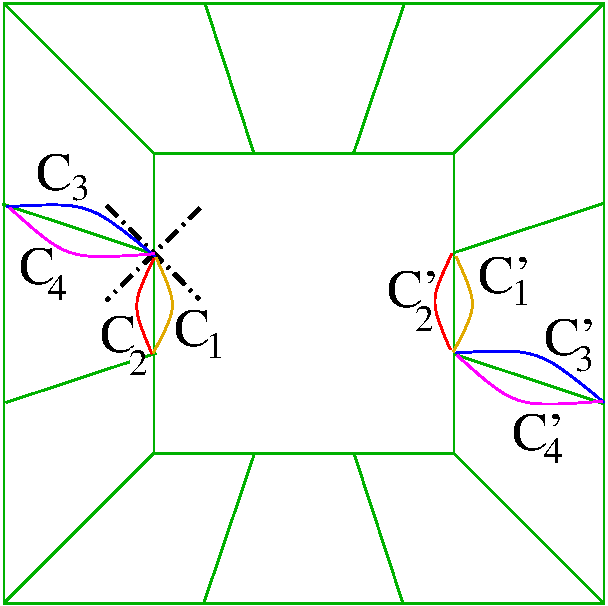
\includegraphics[height=.3\textwidth]{contour_design.pdf}\hspace*{2mm}
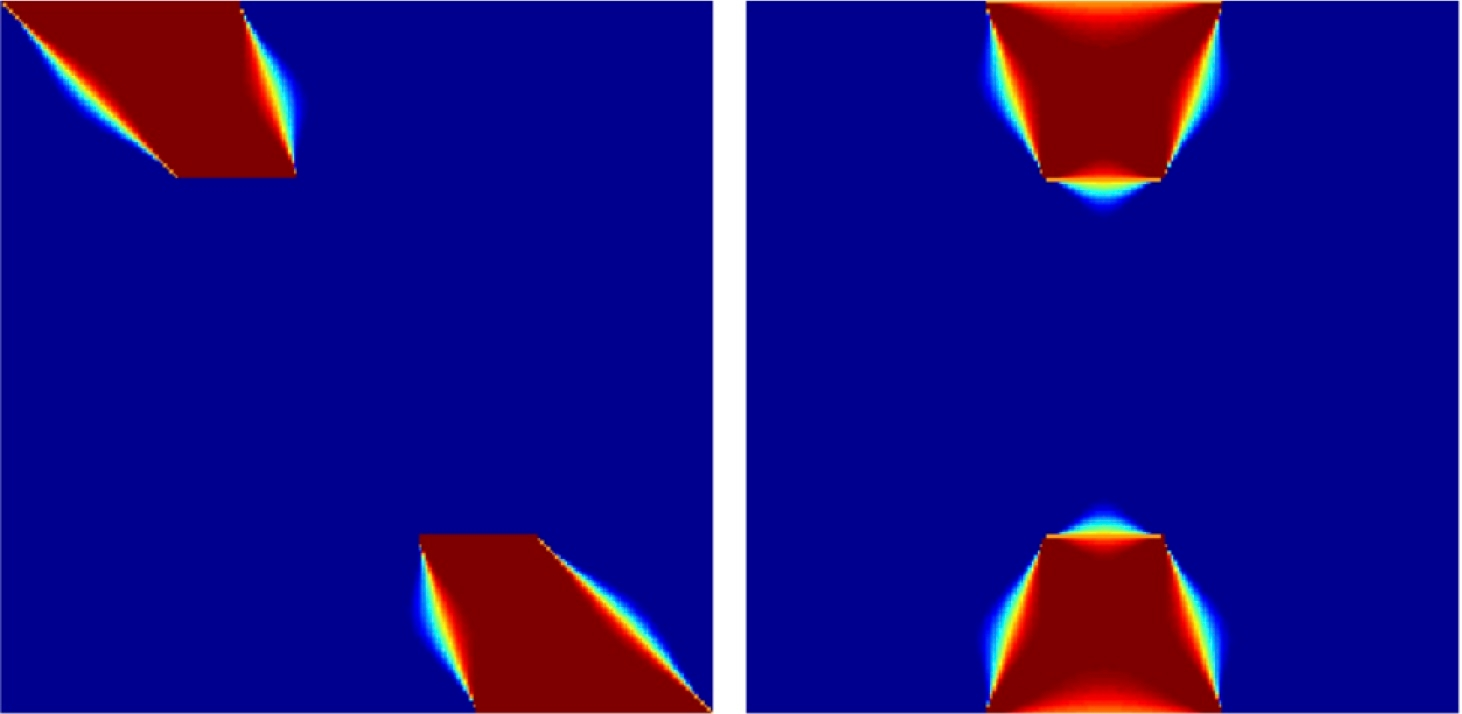
\includegraphics[height=.3\textwidth]{smsh-sh.jpg}
\caption{ Left: contour design of $supp(m_5)$, Right: frequency support $|\hat{\psi}^j|$}
\label{fig: design}
\end{figure}

%\section{Quasi-shearlet bases construction}\label{sec: bases construction}
%In this section, we present a family of quasi-shearlet bases constructed based on the $M$-function design discussed in section \ref{sec: design} using our proposed MRA framework.

We apply this to smooth all the regular boundaries except those on the boundary of $S_0$. Near a regular boundary $\mathcal{B}_{\epsilon}(j,j',\boldsymbol{\pi})$, the discontinuity of $|m_j|$ from 0 to 1 depends on $\mathrm{m}_j$; the contour of stop-band(pass-band) is the boundary of level set $\{\mathrm{m}_j(\boldsymbol{\omega}) = 0\}\,(\{\mathrm{m}_j(\boldsymbol{\omega}) = 1\}$). Fig. \ref{fig: design} shows our design of the stop-band/pass-band contours of regular boundaries {\small $\big(5,6,(\frac{\pi}{2},\frac{\pi}{2})\big)$} and {\small $\big(0,5,(\pi,0)\big)$}. The contours intersect only at the vertices of $C_5$, e.g. $supp(m_5)\cap supp(m_6)\cap supp(m_0)$ contains just one point. % as the relaxed condition (1) in Proposition \ref{prop: pair-smooth}. 
Moreover, we set $\mathrm{m}_5$ to be symmetric with respect to the origin near both regular boundaries. 

The contours related to other regular boundaries are designed likewise to achieve the best symmetry; the corresponding wavelets are real. Fig.\ref{fig: design} (right) shows the frequency support of directional wavelets generated by such design; Fig.\ref{fig: many-squares}(a) shows the wavelets and scaling function in space domain. One easily checks (using Theorem \ref{thm: basis cond}) that this is an orthonormal basis.

\begin{figure}[!t]
\centering
\hspace*{-5mm}\vspace*{-2mm}
\begin{minipage}[t]{\textwidth}
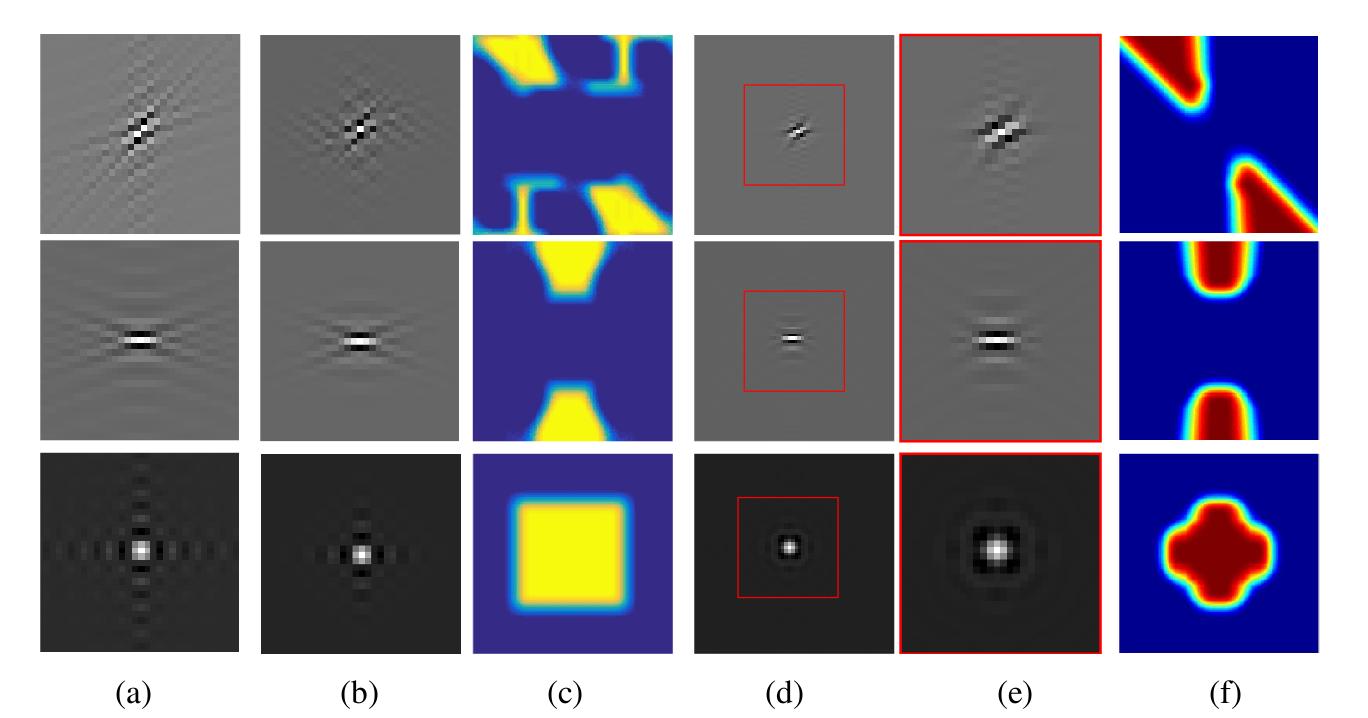
\includegraphics[width=\textwidth]{many_squares_new.png}
\end{minipage}\hspace*{1mm}
\caption{ directional wavelets $\psi^1$, $\psi^2$ and scaling function $\phi$ in different constructions (a) our directional wavelet orthonormal basis, whose frequency support is shown in Fig. \ref{fig: design};(b) Durand's directional wavelet; (c) $m-$ functions of wavelets in (b). (d) our directional wavelet frame; (e) zoom in on (d); (f) $m-$ functions of wavelets in (d);  Our basis construction in (a) has good frequency localization, but slowly decaying spatial oscillation; Durand's construction in (b) has good spatial localization but non-localized frequency support; our frame construction in (d) has both good frequency localization and spatial localization. Note that plots (a),(b),(e) are at the same resolution.}
\label{fig: many-squares}
\vspace*{-3mm}
\end{figure}

Although the wavelets orient in six directions, they are not very well localized spatially, due to the singular boundaries on the corners of the low-frequency square $S_1$, where the discontinuity in the frequency domain is inevitable. The lack of smoothness at the vertices of $m_2$ and $m_5$ could possibly be avoided by using a more delicate (but more complicated) design around the vertices $(\pm\frac{\pi}{2},\pm\frac{\pi}{6})$ allowing triple overlapping of $m-$functions.% yet Proposition \ref{prop: pair-smooth} and consequently Proposition \ref{prop: M-design} are nolonger helpful.

Allowing a bit of redundancy (abandoning critical downsampling), we show next how to construct a frame with low redundancy that has much better spatial localization.
\end{comment}
%\section{Orthonormal Bases}\label{sec: orth}

In this section, we discuss the conditions on $m_j$ such that the corresponding MRA forms an orthonormal bases. 
%consider orthonormal bases with $m-$functions defined in \eqref{eq: m0} and \eqref{eq: mj} whose supports mainly corresponding to the partition of $S_0$ in Fig.\ref{fig: partition}.
%we always consider a multi-resolution system with scaling function $\phi$ and quasi-shearlets $\psi^j$, {\small$ j = 1,\dots,6$} defined by $(M_0, D_2)$ and $(M_j, Q)$, {\small$j = 1,\dots,6$} respectively. Furthermore, the essential support of $M_j$'s corresponds to the partition of $\mathbf{S}_0$ in a shearlet system.

%The construction of \eqref{eq: MRA} reduces to design $m_0$ in \eqref{eq: m0} and $m_j, j= 1,\cdots,6$ in \eqref{eq: mj}.
We begin with the two key conditions, i.e. {\it identity summation} and {\it shift cancellation}, on $m_j$ such that the system \eqref{eq: MRA} is perfect-reconstruction (PR) or equivalently a Parseval frame in MRA.% weaker than the orthonormal condition.

%\subsection{Identity summation and shift cancellation}
\subsection{orthonormal conditions on $m_j$}\label{subsec: northonormal cond}
In MRA, \eqref{eq: MRA} is PR if $\forall f\in L_2(\mathbb{R}^2)$,
\begin{equation}
%\textstyle 
\sum_{\V{k}\in\mathbb{Z}^2}\langle f,\phi_{0,\V{k}}\rangle\phi_{0,\V{k}} = \sum_{\V{k}\in\mathbb{Z}^2}\langle f,\phi_{1,\V{k}}\rangle\phi_{1,\V{k}} + \sum_{j=1}^J\sum_{\V{k}'\in\V{Q}\mathbb{Z}^2}\langle f,\psi^{j}_{1,\V{k}'}\rangle\psi^j_{1,\V{k}'}.\label{eq: PR}
\end{equation}
Using \eqref{eq: m0} and \eqref{eq: mj} together with the admissibility of the frequency partition \eqref{eq: tiling}, condition \eqref{eq: PR} on $\phi$ and $\psi^j$ yields:
\begin{thm}\label{thm: conds}
Let $J=6,\, \V{D} =\bigl(\begin{smallmatrix} 2&0\\0&2\end{smallmatrix}\bigr)$ and $\V{Q}\doteq\bigl(\begin{smallmatrix} 1&1\\-1&1\end{smallmatrix}\bigr)$ in \eqref{eq: MRA}.
Then the perfect reconstruction condition holds for \eqref{eq: MRA} iff the following two conditions hold
\begin{align}\label{eq: id-sum}
|m_0(\boldsymbol{\omega})|^2 + \sum_{j = 1}^6|m_j(\boldsymbol{\omega})|^2 = 1
\end{align}
\begin{equation}\label{eq: shift-cancel}
 \begin{cases}
%M_0(\boldsymbol{omega})\overline{M_0(\boldsymbol{omega}+\boldsymbol{\gamma})} + 
\sum_{j = 0}^6m_j(\boldsymbol{\omega})\overlinespace{m_j}(\boldsymbol{\omega} + \boldsymbol{\pi}) = 0, & \boldsymbol{\pi}\in \Gamma_0\setminus\{\boldsymbol{0}\}\\[.5em]
\sum_{j=1}^6m_j(\boldsymbol{\omega})\overlinespace{m_j}(\boldsymbol{\omega}+\boldsymbol{\pi}) = 0, & \boldsymbol{\pi}\in\Gamma_1\setminus\Gamma_0
\end{cases}
\end{equation}
%where  $\Lambda = (QD\mathbb{Z}^2)^*/(\mathbb{Z}^2)^*,\,\Gamma = (D\mathbb{Z}^2)^*/(\mathbb{Z}^2)^*.$ %$\{(\frac{\pi}{2},\frac{\pi}{2}),(\frac{3\pi}{2},\frac{\pi}{2}),(\frac{\pi}{2},\frac{3\pi}{2}),(\frac{3\pi}{2},\frac{3\pi}{2}),$ $(0,0),(0,\pi),(\pi,0),(\pi,\pi)\}$
\end{thm}

Theorem \ref{thm: conds} is a corollary of Prop. 1 and Prop. 2 in \cite{durand2007}. We give an alternate proof in Appendix \ref{app: cond-thm}.
In Theorem \ref{thm: conds}, Eq. \eqref{eq: id-sum} is the {\it identity summation} condition, guaranteeing conservation of $l_2$ energy; Eq. \eqref{eq: shift-cancel} is the {\it shift cancellation} condition such that aliasing is canceled correctly in reconstruction from wavelet coefficients. %, such that downsampling of scaling and shearlet coefficients is valid. 
 %$\Lambda = \{(\frac{\pi}{2},\frac{\pi}{2}),(\frac{3\pi}{2},\frac{\pi}{2}),(\frac{\pi}{2},\frac{3\pi}{2}),(\frac{3\pi}{2},\frac{3\pi}{2}),$ $(0,0),(0,\pi),(\pi,0),(\pi,\pi)\},\Gamma = \{(0,0),(0,\pi),(\pi,0),(\pi,\pi)\}$ are the sets of shifts associated to quincunx-dyadic dilation $QD$ and dyadic dilation $D$ respectively.
%Each $M_j$ contributes a term $M_j(\boldsymbol{omega})\overline{M_j(\boldsymbol{omega} + \boldsymbol{\nu})}$ in the cancellation condition of any shift $\boldsymbol{\nu}$ corresponding to the downsampling scheme of $M_j$.
Because each $m_j$ is $(2\pi,2\pi)$ periodic, we only need to check these conditions $\forall \V{\omega}\in S_0$.

%\subsection{Extra condition for basis}
%By Theorem \ref{thm: conds}, the system \eqref{eq: MRA} is a Parseval frame ; 
Moreover, for  \eqref{eq: MRA} to be an orthonormal basis,  $\{\phi_{\boldsymbol{k}}\}_{\boldsymbol{k}\in\mathbb{Z}^2}$ need to be an orthonormal basis, which is determined by $m_0$ in \eqref{eq: phi-m0}. In 1D MRA, Cohen's theorem in \cite{cohen1992biorthogonal} provides a necessary and sufficient condition on $m_0$ such that \eqref{eq: MRA} is an orthonormal basis. %Such a condition in 1D wavelet MRA is given by Cohen \cite{cohen1992biorthogonal}. 
This theorem generalizes to 2D as proved in  e.g. \cite{yin2014orthshear}, as follows.
\begin{thm}\label{thm: basis cond}
Assume that $m_0$ is a trigonometric polynomial with $m_0(\V{0})=1$, and define $\hat{\phi}(\boldsymbol{\omega})$ as in \eqref{eq: phi-m0}.\\
If $\phi(\cdot - \boldsymbol{k}),\boldsymbol{k}\in\mathbb{Z}^2$ are orthonormal, then $\exists K$ containing a neighborhood of 0, s.t. $\forall\boldsymbol{\omega}\in S_0,\,\boldsymbol{\omega}+2\pi\mathbf{n}\in K$ for some $\mathbf{n}\in\mathbb{Z}^2, $ and $\inf_{k>0,\,\boldsymbol{\omega}\in K}|m_0(\mathbf{D_2}^{-k}\boldsymbol{\omega})| >0$. 
 Further, if $\sum_{\boldsymbol{\V{\pi}}\in \Gamma_0} |m_0(\boldsymbol{\omega}+\boldsymbol{\pi})|^2 = 1$, then the inverse is true.
\end{thm}
%Theorem \ref{thm: basis cond} can be proved similarly to Cohen's theorem (\cite{cohen1992biorthogonal}).
%Because it is difficult to directly design $M_0$ that satisfies the conditions in Theorem \ref{thm: basis cond}, 
%Below, we construct $m-$functions imposing only \eqref{eq: id-sum} and \eqref{eq: shift-cancel} and then check if the resulting Parseval frame is an orthonormal basis by applying Theorem \ref{thm: basis cond} to $m_0$.

\subsection{Regularity of $m_j$ supported on the $C_j$}\label{sec: design}
%In this section, we define Shannon-type directional orthonormal basis same as in \cite{durand2007} and \cite{nuDFB05}. Then, we apply direct smoothing to its $m-$functions to improve spatial localization, this leads to a critical analysis of the boundary regularity of $S_1$ and the $C_j$'s.

%\subsection{Shannon-type wavelets and smoothing}
In this subsection, we consider $m_j$ supported on the $C_j$ introduced in Section \ref{subsec: frequency partition} that satisfy orthonormal conditions in Section \ref{subsec: northonormal cond}. We begin with the Shannon-type wavelet construction,
where $m_j$ are indicator functions $ m_j = \mathbbm{1}_{C_j},\,0\leq j \leq 6,\,$ and we use the boundary assignment of $C_j$ in Fig.\ref{fig: partition}.
The identity summation follows from the partition of $S_0$ by the $C_j$, and the shift cancellation follows from the tiling property \eqref{eq: tiling}. % which implies $m_j(\boldsymbol{\omega})\overline{m_j(\boldsymbol{\omega} + \boldsymbol{\pi}_i)}\equiv 0,\,\forall j,\, i\neq 0.$ %Let $\partial\mathbf{C}_j = \overline{\mathbf{C}_j}-\mathbf{C}_j^{\circ}$ be the boundary of $\mathbf{C}_j$,  
Applying Theorem \ref{thm: basis cond} to $m_0$, we verify that the Shannon-type wavelets generated from these $m_j$ form an orthonormal basis.

%However, because of the discontinuity of $m_j$ across the boundary of its support, the corresponding wavelet has slow decay in the time domain. 
%Such $m_j$'s are not regularized due to 
Because of the discontinuity at $\partial C_j$, the boundaries of the $C_j$, these $m_j$ are not smooth, and hence the corresponding wavelets are not spatially localized. The $m_j$ can be regularized by smoothing at the $\partial C_j$.
%We take a different regularization approach from Durand's \cite{durand2007}, where three regular quincunx filter banks are constructed and then composed to obtain the desired regular quincunx dyadic filter banks. Here, we smooth the discontinuous boundaries of $m-$functions directly. 
However, as shown in Proposition 3 in \cite{durand2007}, it is not possible to smooth the behavior of the $m_j$ at  {\it all} the boundaries with discontinuity if the $m_j$ have to satisfy the perfect reconstruction condition.
In \cite{yin2014orthshear}, the $\partial C_j$ are segmented into {\it singular} and {\it regular} pieces. On regular boundaries, pairs of $(m_j,\, m_{j'})$ share a boundary and can both be smoothed in a coherent way such that all the constraints in Theorem \ref{thm: basis cond} remain satisfied. The singular pieces are boundaries for just one $m_j$, which can then not be smoothed without violating the shift cancellation condition. Fig. \ref{fig: boundary} shows the boundary classification, where the corners of $S_0$ and $C_0$ are singular, hence $m_0$ and the $m_j$'s in two diagonal directions of an orthonormal bases are discontinuous there. A mechanism of constructing orthonormal bases by smoothing Shannon-type $m_j$ on regular boundaries is provided in \cite{yin2014orthshear}.%However, it remains unclear if some of the discontinuity can be removed by direct smoothing.

%Next, we analyze the limitation of direct smoothing in detail and show that there are regular boundaries which can be smoothed without violating \eqref{eq: id-sum} and \eqref{eq: shift-cancel}, and singular boundaries which cannot be smoothed.

%\textcolor{red}{In the remainder of this paper, we explore how this can be done for the first dyadic layer (without cutting further at higher frequencies); we call the corresponding basis {\it quasi-Shearlets}.}

\begin{figure}[!t]
\centering
%\hspace*{-5mm}
%\begin{minipage}{.6\textwidth}
%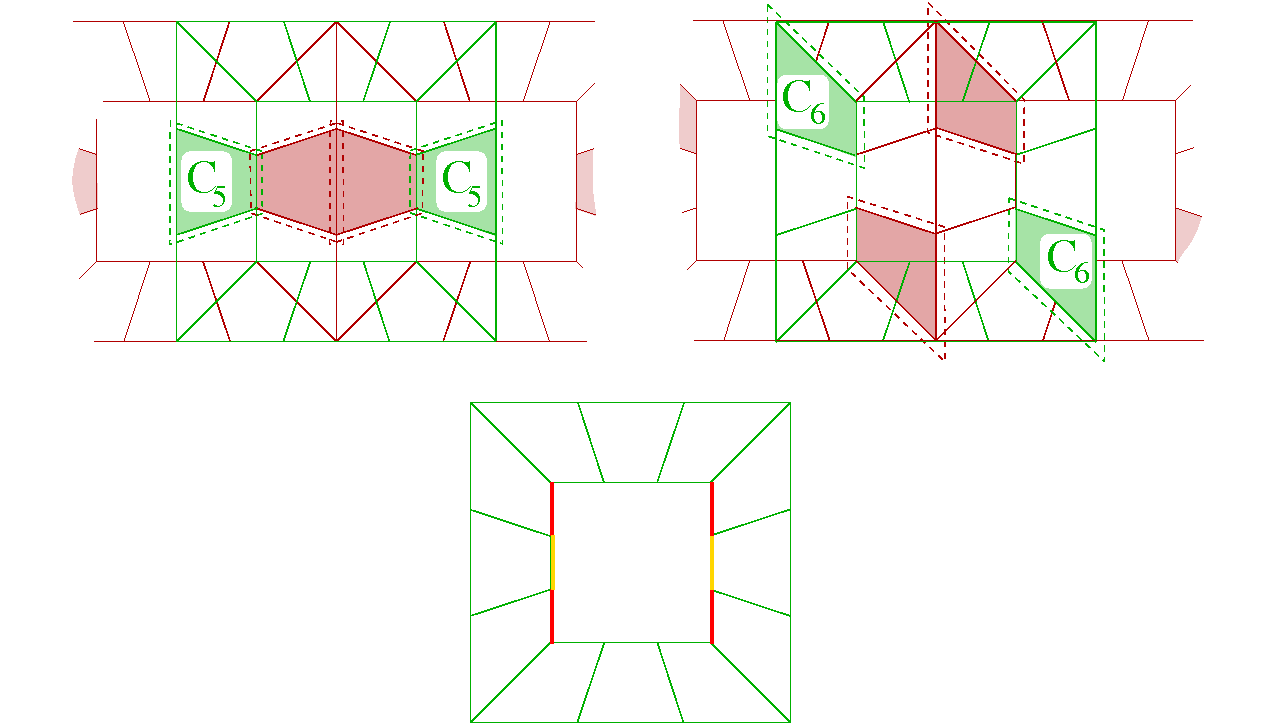
\includegraphics[width=\textwidth]{fig_overlap.png}\hspace*{-2mm}
%\end{minipage}
\begin{minipage}{.3\textwidth}
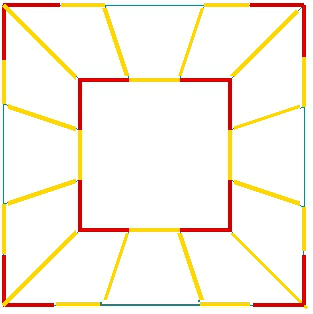
\includegraphics[width=\textwidth]{bdyclass.jpg}
\end{minipage}
%\includegraphics[width=.2\textwidth]{fig/sublattice-2.jpg}
\caption[caption]{
%\textcolor{red}{
%{\it Left top}: the supports of $m_j$ (green) and $m_j(\cdot+\V{\pi}_2$ (red) for $j = 5,6$ after smoothing, overlap on the vertical boundary at $\omega_1 =  \pm \pi/2$ of $C_5$ (green) and its shift (red) by $\boldsymbol{\pi}_2 = (\pi,0)$. Note that two copies of shifted $S_0$ (red) overlap the un-shifted $S_0$(green) due to the $(2\pi,2\pi)$ periodicity of $m_j$. Only $m_0$ and $m_5$ have overlapping smoothed boundaries by $\boldsymbol{\pi}_2$. 
%\\\hspace{\textwidth}
%{\it Left bottom}: intersection of $\mathcal{B}(0,\boldsymbol{\pi}_2)$ and $\mathcal{B}(5,\boldsymbol{\pi}_2)$ in yellow and $\mathcal{C}(0,\boldsymbol{\pi}_2) = \mathcal{B}(0,\boldsymbol{\pi}_2)\setminus\mathcal{B}(5,\boldsymbol{\pi}_2)$ in red. Smoothing $m_0$ in the red (singular) region is impossible without violating \eqref{eq: shift-cancel}. %This leads to the distinction between regular (yellow) and singular (red) boundaries at $omega_1 = \pm\pi/2$.
%\\\hspace{\textwidth}
%{\it Right}: 
Boundary classification, singular (red) and regular (yellow) }%after similar arguments for all shifts $\boldsymbol{\pi}_i$.}
 %}
\label{fig: boundary}
\end{figure}

\begin{comment}
%\subsection{Boundary classification}
 After smoothing the $m_j$'s, the shift cancellation \eqref{eq: shift-cancel} may fail to hold as $supp(m_j)$ and $(supp(m_j)-\boldsymbol{\pi})$ may overlap near the smoothed boundaries, see Fig. \ref{fig: boundary}, illustrating $m_5(\boldsymbol{\omega})\overline{m_5(\boldsymbol{\omega} + \boldsymbol{\pi}_2)}\not\equiv 0.$
For simplicity, we introduce the following notations: let 
$\mathcal{B}(j,\boldsymbol{\pi}) =  supp(m_j)\cap\,(supp(m_j)-\boldsymbol{\pi})$ be the support of  $m_j(\boldsymbol{\omega})\overline{m_j(\boldsymbol{\omega} + \boldsymbol{\pi})}$ associated to $m_j$ and shift $\boldsymbol{\pi}$;
let $\mathcal{C}(j,\boldsymbol{\pi}) = \mathcal{B}(j,\boldsymbol{\pi}) \setminus \bigcup_{j'\neq j}\mathcal{B}(j',\boldsymbol{\pi})$. 
%In addition, we may introduce the (slight abuse of) notation $C_0 = S_1$.
\begin{lem}\label{lem: singular-bdy}
Shift cancellation \eqref{eq: shift-cancel} can hold for shift $\boldsymbol{\pi}\in\Gamma_0\setminus\{\boldsymbol{0}\}$, only if $\mathcal{C}(j,\boldsymbol{\pi})=\varnothing,\, \forall\, 0\leq j\leq 6$; 
it can hold for shift $\boldsymbol{\pi}\in\Gamma_1\setminus\Gamma_0$, only if $\mathcal{C}(j,\boldsymbol{\pi})=\varnothing,\, \forall\, 1\leq j\leq 6$. 
\end{lem}
\noindent{\it Proof.} Observe that, on $\mathcal{C}(j,\boldsymbol{\pi})$, $m_j(\boldsymbol{\omega})\overline{m_{j}(\boldsymbol{\omega}+\boldsymbol{\pi})} \not\equiv 0$ but $m_{j'}(\boldsymbol{\omega})\overline{m_{j'}(\boldsymbol{\omega}+\boldsymbol{\pi})} \equiv 0,\, \forall j' \neq j$, hence \eqref{eq: shift-cancel} doesn't hold. $\hfill\square$
%Furthermore, the identity summation constraint \eqref{eq: id-sum} implies that $|M_j(\boldsymbol{omega})| = 1$ on $\mathcal{C}(j,\boldsymbol{\nu}),\,\forall\boldsymbol{\nu}$, hence the discontinuity of $M$-functions across these boundaries is unavoidable.
 
Therefore, boundaries that after smoothing make $\mathcal{C}(j,\boldsymbol{\pi})$ non-empty are called {\it singular}; the rest are {\it regular}. We next provide an explicit boundary classification method:
\begin{prop}\label{prop: class-bdy}
$\forall\, 1\leq j\leq 6$, let $supp(m_j) = \ov{$C_j$}$, then the boundary of $C_j$ is $\partial C_j=\bigcup_{i \neq 0}\mathcal{B}(j,\boldsymbol{\pi}_i)$. The set of singular boundaries of $\partial C_j$ is $\bigcup_{i\neq 0}\mathcal{C}(j,\boldsymbol{\pi}_i)$, whereas its compliment set is the regular boundary set.
 \end{prop}
\noindent{\it Proof.} Since $\bigcup_i(C_j+\boldsymbol{\pi}_i) = S_0$, $\partial C_j\subset \bigcup_{i\neq 0} (\ov{$C_j$}+\boldsymbol{\pi}_i) $. Therefore, $\partial C_j\subset\bigcup_{i\neq 0}\mathcal{B}(j,\boldsymbol{\pi}_i)$. On the other hand, $\mathcal{B}(j,\boldsymbol{\pi}_i)\subset \partial\mathbf{C}_j, \forall \, i\neq 0$, hence the union of them is a subset of $\partial C_j$. It follows that $\mathcal{B}(j,\boldsymbol{\pi}_i)$ form a partition of the boundary $\partial C_j$. The partition of $\partial C_j$ into singular and regular boundaries follows from Lemma \ref{lem: singular-bdy}.$\hfill\square$

 The case of $\partial S_1$ is similar where $\mathcal{B}(0,\boldsymbol{\pi}),\,\boldsymbol{\pi}\in\Gamma_0\setminus\{0\}$ are considered. We use the notation $\mathcal{B}_s(j,\boldsymbol{\pi}),\mathcal{C}_s(j,\boldsymbol{\pi})$ for the special case $supp(m_j) = \ov{$C_j$}$ hereafter.
The boundary classification based on Proposition \ref{prop: class-bdy} is shown in the right of Fig. \ref{fig: boundary}, where the boundaries on the four corners of both $S_0$ and $S_1$ are singular: smoothing is then not allowed there.

\begin{prop}\label{prop: jump}
Let $\mathcal{C} = \mathcal{C}_s(j_1,\boldsymbol{\pi}_{i_1})\cap \mathcal{C}_s(j_2,\boldsymbol{\pi}_{i_2})$, if $m_{j_1}, m_{j_2}$ satisfy \eqref{eq: id-sum}, \eqref{eq: shift-cancel}, then $|m_{j_1}|=\mathbbm{1}_{\mathbf{C}_{j_1}},\,|m_{j_2}|=\mathbbm{1}_{\mathbf{C}_{j_2}}$ on $\mathcal{C}$.
\end{prop}
\noindent{\it Proof.} Suppose the common singular boundary $\mathcal{C}$ is non-empty and observe that $\mathcal{C}\subset(C_{j_1})\cap(C_{j_2})$. Since $m_{j_1}$ cannot be smoothed on $\mathcal{C}_s(j_1,\boldsymbol{\pi}_{i_1})$, $|m_{j_1}| = 0$ on $\mathcal{C}_s(j_1,\boldsymbol{\pi}_{i_1})\setminus\mathbf{C}_{j_1}$, 
%Because $\mathcal{C}\subset\mathcal{C}_s(j_1,\boldsymbol{\nu}_1)\cap\partial\mathbf{C}_{j_2}$, 
and \eqref{eq: id-sum} implies that $|m_{j_2}| = 1$ there, or equivalently $|m_{j_2}|=\mathbbm{1}_{\mathbf{C}_{j_2}}$ on $\mathcal{C}$. Similarly, $|m_{j_1}|=\mathbbm{1}_{\mathbf{C}_{j_1}}$ on $\mathcal{C}.\hfill\square$

Prop. \ref{prop: jump} shows that if $m_j$ and $m_{j'}$ have common singular boundaries, then both will have a discontinuity across those boundaries. For example, $\mathcal{C}_s(0,(\pi,0))\cap\mathcal{C}_s(4,(\pi/2,\pi/2)) = (\pi/2,(\pi/6,\pi/2))$, hence $m_0$ and $m_4$ both are discontinuous at $(\pi/2,(\pi/6,\pi/2))$. All the singular boundaries related to \eqref{eq: MRA} are such "double" singular boundaries.

\subsection{Pairwise smoothing of regular boundary}
%Despite of the singular boundaries, better spatial localization can be achieved by carefully smoothing the regular boundaries. 
The regular boundaries of both $C_{j_1}$ and $C_{j_2}$ with adjacent supports consist of $\mathcal{B}_s(j_1,\boldsymbol{\pi})\cap\mathcal{B}_s(j_2,\boldsymbol{\pi})$, which we denote by the triple $(j_1,j_2,\boldsymbol{\pi})$. The following proposition shows that the regular boundaries $(j_1,j_2,\boldsymbol{\pi})$ can be paired according to shift pairs $(\boldsymbol{\pi},-\boldsymbol{\pi})$, and the boundaries must be smoothed pairwise within their $\epsilon-$neighborhood, $\mathcal{B}_{\epsilon}(j_1,j_2,\boldsymbol{\pi})$ and $\mathcal{B}_{\epsilon}(j_1,j_2,-\boldsymbol{\pi})$.

\begin{prop}\label{prop: pair-smooth}
Given $(j_1,j_2,\boldsymbol{\pi})\neq \varnothing$, %let $\boldsymbol{\nu}'= -\boldsymbol{\nu}\in \mathbb{R}^2/(\mathbb{Z}^2)^*$, 
then $(j_1,j_2,-\boldsymbol{\pi})\neq\varnothing$. In addition, let $\mathcal{B}=\mathcal{B}_{\epsilon}(j_1,j_2,\boldsymbol{\pi})\cup\mathcal{B}_{\epsilon}(j_1,j_2,-\boldsymbol{\pi})$. Then the identity summation and shift cancellation conditions hold if
\begin{itemize}
\item[{\it (i)}] $m_j = \mathbbm{1}_{C_j},\quad\text{on }S_0,\; j\neq j_1,j_2$
\item[{\it (ii)}] $m_{j_1} =\mathbbm{1}_{C_{j_1}},\, m_{j_2} =\mathbbm{1}_{C_{j_2}},\quad \text{on }\mathcal{B}^c$\\[.5em]
\hspace*{-2em} and on $\mathcal{B}$ the following hold%\vspace*{.1em}
\item[{\it(iii)}] $|m_{j_1}|^2 + |m_{j_2}|^2 = 1,$ %\hfill on $ \mathcal{B}_{\epsilon}(j_1,j_2,\nu)\cup\mathcal{B}_{\epsilon}(j_1,j_2,\nu')$
\item[{\it (iv)}] $\sum_{j_1,j_2} m_j(\cdot)\overline{m_j(\cdot+\widetilde{\boldsymbol{\pi}})} = 0,\, \widetilde{\boldsymbol{\pi}} = \pm\boldsymbol{\pi}$
%\hspace*{8em} on $\mathcal{B}_{\epsilon}(j_1,j_2,\nu)$ and $\mathcal{B}_{\epsilon}(j_1,j_2,\nu)-\nu$
%\item[{\it (v)}] $\sum_{j_1,j_2} M_j(\cdot)\overline{M_j(\cdot+\boldsymbol{\nu}')} = 0.$ 
%\hspace*{7em} on $\mathcal{B}_{\epsilon}(j_1,j_2,\boldsymbol{\nu}')$ and $\mathcal{B}_{\epsilon}(j_1,j_2,\nu')-\nu'$
\end{itemize}
\end{prop}
\noindent{\it Proof}.
 We first show that $(j_1,j_2,-\boldsymbol{\pi})\neq\varnothing.$ By definition, $\mathcal{B}_s(j_1,\boldsymbol{\pi}) = supp(m_{j_1})\cap (supp(m_{j_1})-\boldsymbol{\pi}) = \left((supp(m_{j_1})+\boldsymbol{\pi})\cap supp(m_{j_1})\right)-\boldsymbol{\pi} = \mathcal{B}_s(j_1,-\boldsymbol{\pi})-\boldsymbol{\pi}.$ Rewrite $(j_1,j_2,\boldsymbol{\pi})$ by $\mathcal{B}_s(j_1,-\boldsymbol{\pi})$ and $\mathcal{B}_s(j_2,-\boldsymbol{\pi})$, we have $(j_1,j_2,-\boldsymbol{\pi}) = (j_1,j_2,\boldsymbol{\pi})+\boldsymbol{\pi}$, hence it's non-empty.
 
Because $(j_1,j_2,\pm\boldsymbol{\pi})\subset (\partial C_{j_1} \bigcap \partial C_{j_2})$ and $(\bigcup_{j}C_j)=S_0$, $(\bigcup_{j\neq j_1,j_2}C_j)\cap \mathcal{B} = \varnothing.$ Therefore, smoothing of $m_{j_1}$ and $m_{j_2}$ in $\mathcal{B}$ doesn't impact the region where other $m_j$'s are supported.

We then show that the cancellation conditions \eqref{eq: shift-cancel} hold for all shifts. Condition (i) and (ii) imply that $\mathcal{B}(j,\widetilde{\boldsymbol{\pi}})= \varnothing,\,\forall j,\widetilde{\boldsymbol{\pi}}\neq \pm \boldsymbol{\pi}$, hence \eqref{eq: shift-cancel} hold for $\widetilde{\boldsymbol{\pi}}\neq \pm \boldsymbol{\pi}$. %For $\boldsymbol{\nu}$, 
(i) implies $\mathcal{B}(j,\widetilde{\boldsymbol{\pi}}) = \varnothing,\,\forall j\neq j_1,j_2$, so then \eqref{eq: shift-cancel} is equivalent to (iv). %Similarly, \eqref{eq: shift-cancel} is equivalent to (v) under (i).
The identity summation \eqref{eq: id-sum} holds due to (i), (ii) and (iii).$\hfill\square$.

By Prop. \ref{prop: pair-smooth} we can smooth some pairs of regular boundaries starting from the Shannon-type directional wavelets with the simplified conditions (iii), (iv) and (v); (i) and (ii) can be removed as long as the initial $m_j$ satisfy \eqref{eq: id-sum} and \eqref{eq: shift-cancel} and every $\boldsymbol{\omega}\in S_0$ is not covered by more than two $m$ functions. We can thus smooth regular boundaries pairwise, one by one.

The next proposition gives an explicit design of $(m_{j_1}, m_{j_2})$ satisfying the simplified conditions (iii),(iv) in Proposition \ref{prop: pair-smooth}. %as well as a necessary condition for any valid design.
\begin{prop}\label{prop: m-design}
Let $C\subset S_0$, given $m_{j_1},m_{j_2}\neq 0$ continuous on $ C\cup(C+\boldsymbol{\pi})$, satisfying the following conditions
\begin{itemize}
\item[(i)] $\sum_{j_1,j_2}m_{j}(\boldsymbol{\omega})\overline{m_{j}(\boldsymbol{\omega}+\boldsymbol{\pi})} = 0$ \hspace*{2em} on $C$
\item[(ii)] $\sum_{j_1,j_2}|m_{j}(\boldsymbol{\omega})|^2= 1 $ \hspace*{5em} on $C\cup (C+\boldsymbol{\pi})$
\item[(iii)] $m_{j_1}(\boldsymbol{\omega})m_{j_2}(\boldsymbol{\omega}) = 0$\hspace*{5em} on $\partial C$ ;
\end{itemize}
then
$\quad|m_{j_1}(\boldsymbol{\omega})| = |m_{j_2}(\boldsymbol{\omega}+\boldsymbol{\pi})|,\quad |m_{j_2}(\boldsymbol{\omega})| = |m_{j_1}(\boldsymbol{\omega}+\boldsymbol{\pi})|.$\\[1mm]
Furthermore, if $m_{j} = e^{i\boldsymbol{\omega}^{T}\boldsymbol{\eta}_{j}}\mathrm{m}_{j},\quad j=j_1,j_2, \text{ on }C,$ where $\mathrm{m}_j$ is a real-valued function, % $\mathcal{M}_{j_1}$ and $\mathcal{M}_{j_2}$,  phase $\eta_1,\eta_2$ s.t.
$e^{i\boldsymbol{\pi}^T(\boldsymbol{\eta}_{j1}-\boldsymbol{\eta}_{j2})} = -1,$ and 
\[\mathrm{m}_{j_1}(\boldsymbol{\omega}) = \mathrm{m}_{j_2}(\boldsymbol{\omega}-\boldsymbol{\pi}),\;\mathrm{m}_{j_2}(\boldsymbol{\omega}) = \mathrm{m}_{j_1}(\boldsymbol{\omega}-\boldsymbol{\pi}),\text{ on }C+\boldsymbol{\pi},\] 
%where $\mathcal{M}_{j1},\,\mathcal{M}_{j2}$ are 
then $(i)$ holds.
\end{prop}
\noindent{\it Proof.} 
To prove the necessary condition, note that (i) implies $|m_{j_1}(\boldsymbol{\omega})|^2|m_{j_1}(\boldsymbol{\omega+\pi})|^2 = |m_{j_2}(\boldsymbol{\omega})|^2|m_{j_2}(\boldsymbol{\omega+\pi})|^2$; the condition then follows from (ii).
For the sufficient construction, check by directly substituting the construction into (i). $\hfill\square$
%For the necessary condition, we prove in two cases. Suppose $|M_{j_1}|  = |M_{j_2}|$ on $\omega$, then (ii) implies $|M_{j_1}| = |M_{j_2}| = \frac{1}{2}$ on $\omega$. From (i), it's necessary $|M_{j_1}(\boldsymbol{omega}+\boldsymbol{\nu})|=|M_{j_2}(\boldsymbol{omega}+\boldsymbol{\nu})|$ on $\omega$, or equivalently, $|M_{j_1}| = |M_{j_2}|$ on $\omega + \boldsymbol{\nu}$. Apply (ii) again, we have $|M_{j_1}| = |M_{j_2}| = \frac{1}{2}$ on $\omega+\boldsymbol{\nu}$, therefore, $|M_{j_1}(\boldsymbol{omega})| = |M_{j_2}(\boldsymbol{omega}+\boldsymbol{\nu})|=|M_{j_2}(\boldsymbol{omega})| = |M_{j_1}(\boldsymbol{omega}+\boldsymbol{\nu})|=\frac{1}{2}.$%However, (iii) implies that either $M_{j_1}$ or $M_{j_2}$ decays to zero on the boundary, therefore, $|M_{j_1}$ and $|M_{j_2}|$ cannot be constant.

%Suppose now $|M_{j_1}(\boldsymbol{omega})| = |M_{j_2}(\boldsymbol{omega}+\boldsymbol{\nu})|$ on $\omega$, then (i) implies $|M_{j_2}(\boldsymbol{omega})| = |M_{j_1}(\boldsymbol{omega}+\boldsymbol{\nu})|$ on $\omega$.


Proposition \ref{prop: m-design} breaks down the design of $(m_{j_1},m_{j_2})$ into a pair of real functions $(\mathrm{m}_{j_1}, \mathrm{m}_{j_2})$ on $\mathcal{B}_{\epsilon}(j_1,j_2,\boldsymbol{\pi})$ and two vectors $\boldsymbol{\eta}_1,\boldsymbol{\eta}_2$; then $(\mathrm{m}_{j_1}, \mathrm{m}_{j_2})$ on $\mathcal{B}_{\epsilon}(j_1,j_2,-\boldsymbol{\pi})$ are automatically determined. %When all regular boundaries adopt this smoothing scheme,  each $\mathcal{M}_j$ has to locally match up with every $\mathcal{M}_{j'}$'s that shares a regular boundary $(j,j',\nu)$. Therefore, we may focus on 
The only constraint on $(\mathrm{m}_{j_1},\mathrm{m}_{j_2})$ for (ii) in Proposition \ref{prop: m-design} to hold is that on $\mathcal{B}_{\epsilon}(j_1,j_2,\boldsymbol{\pi})$, $\sum_{j_1,j_2}|\mathrm{m}_{j}(\boldsymbol{\omega})|^2= 1$, which is easy to be satisfied.
We may construct all local pairs of $(\mathrm{m}_{j_1},\mathrm{m}_{j_2})$ separately, and put together afterwards different pieces of each $\mathrm{m}_j$ located in different regular boundary neighborhoods $\mathcal{B}_{\epsilon}(j,j',\boldsymbol{\pi})$. 

\vspace*{.2em}
%The phase term $e^{i\boldsymbol{omega}^T\boldsymbol{\eta}_j}$ is preferably defined on the full frequency domain, hence $\boldsymbol{\eta}_j$'s need to be solved globally. This global phase problem is stated precisely in t
The next proposition gives % conditions for the $\boldsymbol{\eta}_j$ as well as 
one solution, easy to verify.
\begin{prop}\label{prop: phase}
Applying Proposition \ref{prop: m-design} to all regular boundaries requires a set of phases $\{\boldsymbol{\eta}_j\}_{j = 0}^6,$ s.t.\[\textstyle e^{i\boldsymbol{\nu}^T(\boldsymbol{\eta}_{j1}-\boldsymbol{\eta}_{j2})} = -1, \quad\forall (j_1,j_2,\boldsymbol{\pi})\in\Delta,\]
{\small\begin{multline*}
\Delta = \Bigl\{\big(0,2,(0,\pi)\big),\, \big(0,5,(\pi,0)\big),\,\big(1,3,(\pi,0)\big),\,\big(4,6,(0,\pi)\big),\\
\big(1,6,(\pi/2, 3\pi/2)\big),\,\big(2,3,(\pi/2, 3\pi/2)\big),\,\big(4,5,(\pi/2, 3\pi/2)\big), \\
\big(3,4,(\pi/2, \pi/2)\big),\big(1,2,(\pi/2, \pi/2)\big),\,\big(5,6,(\pi/2, \pi/2)\big)\Bigr\}
\end{multline*}}
The following is a (non-unique) solution: 
{\small\begin{multline*}\boldsymbol{\eta}_0 = (0,0),\,\boldsymbol{\eta}_1 = (0,0),\,\boldsymbol{\eta}_2 = (1,1),\,\boldsymbol{\eta}_3 = (1,-1),\\
\boldsymbol{\eta}_4 = (0,2),\,\boldsymbol{\eta}_5=(1,1),\,\boldsymbol{\eta}_6 = (-1,1).
\end{multline*}}
\end{prop}

To summarize, Proposition \ref{prop: m-design} and \ref{prop: phase} introduce the following regular boundary smoothing scheme for the $m$ functions:
\begin{description}% prevent items from splitting
\item[construction of orthonormal basis]\
\begin{itemize}
\item[1.] First, set $\mathrm{m}_j = \mathbbm{1}_{C_j}$; then smoothen these across a pair of regular boundaries $(j_1,j_2,\pm\boldsymbol{\pi})$ following steps 2, 3.
\item[2.]  On $\mathcal{B}_{\epsilon}(j_1,j_2,\boldsymbol{\pi})$,\\
\hspace*{2em} design $(\mathrm{m}_{j_1},\mathrm{m}_{j_2}),\quad$ s.t.
$\sum_{j_1,j_2}|\mathrm{m}_{j}(\boldsymbol{\omega})|^2= 1$.
\item[3.] On $\mathcal{B}_{\epsilon}(j_1,j_2,-\boldsymbol{\pi})$, \\
\hspace*{2em}let $\mathrm{m}_{j_1}(\boldsymbol{\omega}) = \mathrm{m}_{j_2}(\boldsymbol{\omega}-\boldsymbol{\pi})$, $\mathrm{m}_{j_2}(\boldsymbol{\omega}) = \mathrm{m}_{j_1}(\boldsymbol{\omega}-\boldsymbol{\pi})$\vspace*{.1em}
\item[4.] Repeat step 2 and 3 for all $(j_1,j_2,\boldsymbol{\pi})\in\Delta$. 
\item[5.]$m_j(\boldsymbol{\omega}) =e^{i\boldsymbol{\omega}^T\boldsymbol{\eta}_j} \mathrm{m}_j(\boldsymbol{\omega}),$ on $S_0$, with the $\boldsymbol{\eta}_j$ of Prop. \ref{prop: phase}.
\end{itemize}
\end{description}

\begin{figure}[!t]
\centering
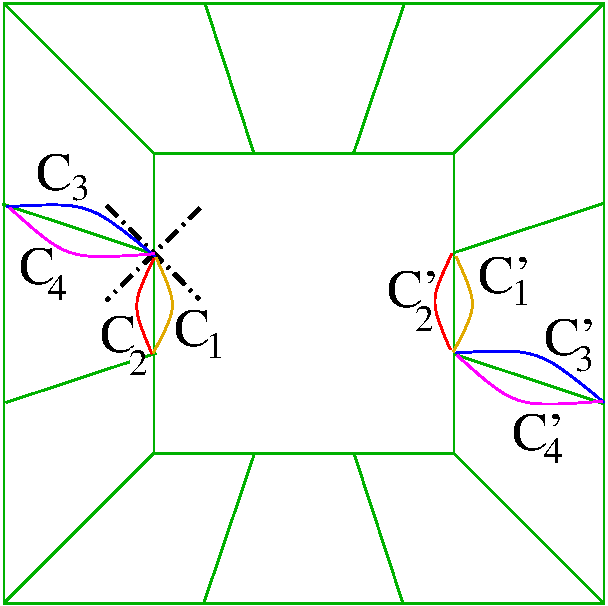
\includegraphics[height=.3\textwidth]{contour_design.pdf}\hspace*{2mm}
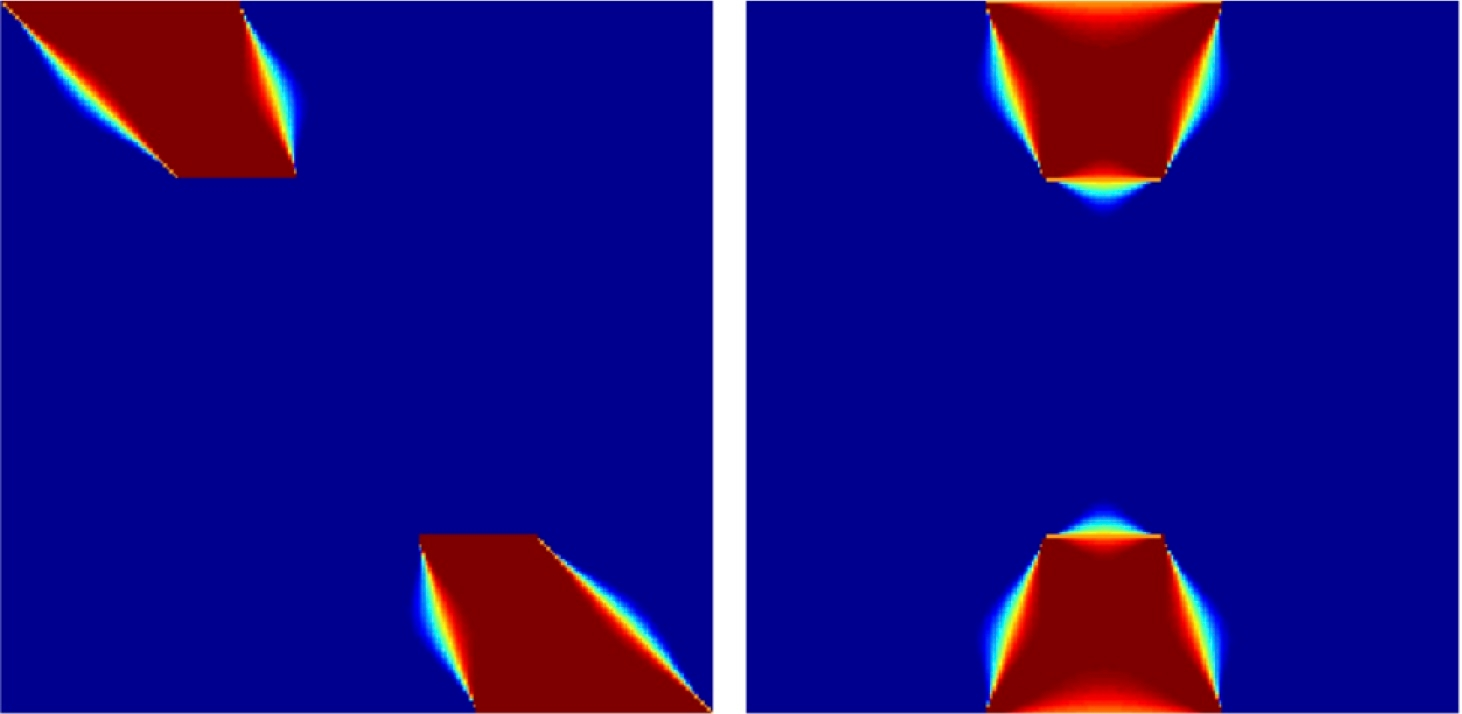
\includegraphics[height=.3\textwidth]{smsh-sh.jpg}
\caption{ Left: contour design of $supp(m_5)$, Right: frequency support $|\hat{\psi}^j|$}
\label{fig: design}
\end{figure}

%\section{Quasi-shearlet bases construction}\label{sec: bases construction}
%In this section, we present a family of quasi-shearlet bases constructed based on the $M$-function design discussed in section \ref{sec: design} using our proposed MRA framework.

We apply this to smooth all the regular boundaries except those on the boundary of $S_0$. Near a regular boundary $\mathcal{B}_{\epsilon}(j,j',\boldsymbol{\pi})$, the discontinuity of $|m_j|$ from 0 to 1 depends on $\mathrm{m}_j$; the contour of stop-band(pass-band) is the boundary of level set $\{\mathrm{m}_j(\boldsymbol{\omega}) = 0\}\,(\{\mathrm{m}_j(\boldsymbol{\omega}) = 1\}$). Fig. \ref{fig: design} shows our design of the stop-band/pass-band contours of regular boundaries {\small $\big(5,6,(\frac{\pi}{2},\frac{\pi}{2})\big)$} and {\small $\big(0,5,(\pi,0)\big)$}. The contours intersect only at the vertices of $C_5$, e.g. $supp(m_5)\cap supp(m_6)\cap supp(m_0)$ contains just one point. % as the relaxed condition (1) in Proposition \ref{prop: pair-smooth}. 
Moreover, we set $\mathrm{m}_5$ to be symmetric with respect to the origin near both regular boundaries. 

The contours related to other regular boundaries are designed likewise to achieve the best symmetry; the corresponding wavelets are real. Fig.\ref{fig: design} (right) shows the frequency support of directional wavelets generated by such design; Fig.\ref{fig: many-squares}(a) shows the wavelets and scaling function in space domain. One easily checks (using Theorem \ref{thm: basis cond}) that this is an orthonormal basis.

\begin{figure}[!t]
\centering
\hspace*{-5mm}\vspace*{-2mm}
\begin{minipage}[t]{\textwidth}
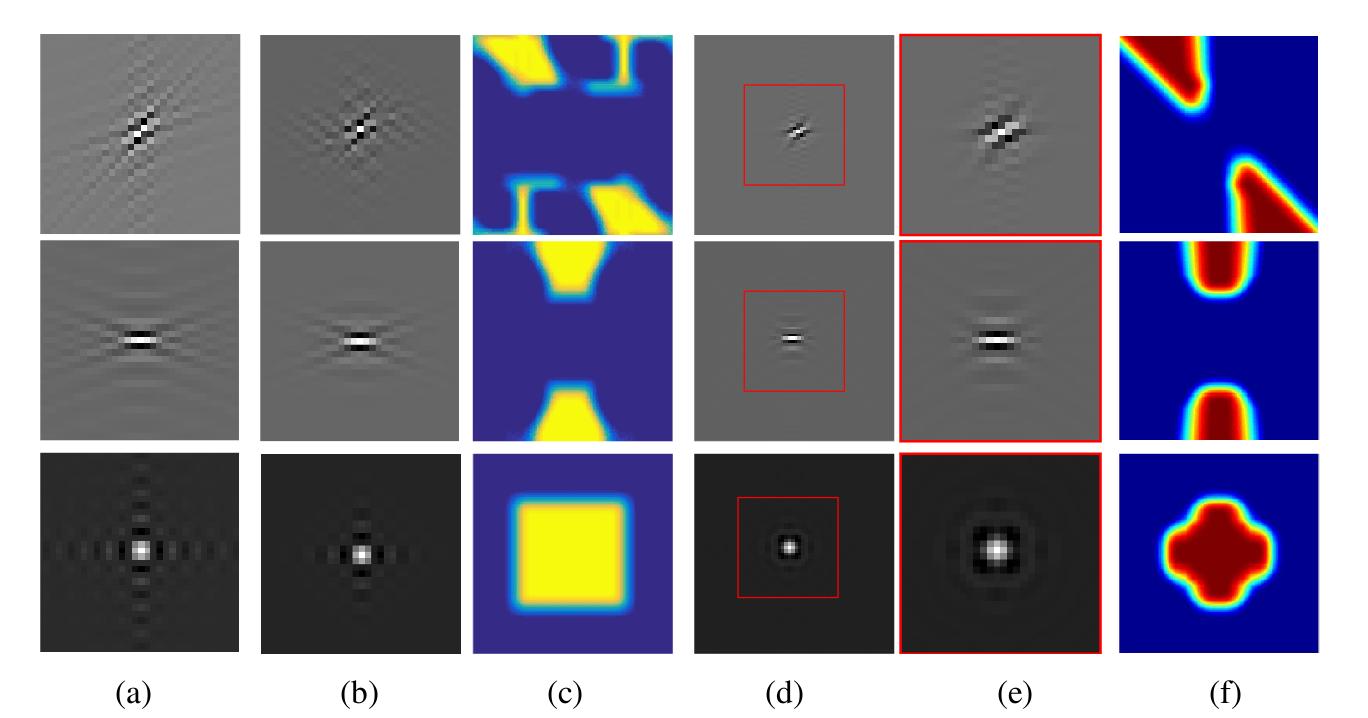
\includegraphics[width=\textwidth]{many_squares_new.png}
\end{minipage}\hspace*{1mm}
\caption{ directional wavelets $\psi^1$, $\psi^2$ and scaling function $\phi$ in different constructions (a) our directional wavelet orthonormal basis, whose frequency support is shown in Fig. \ref{fig: design};(b) Durand's directional wavelet; (c) $m-$ functions of wavelets in (b). (d) our directional wavelet frame; (e) zoom in on (d); (f) $m-$ functions of wavelets in (d);  Our basis construction in (a) has good frequency localization, but slowly decaying spatial oscillation; Durand's construction in (b) has good spatial localization but non-localized frequency support; our frame construction in (d) has both good frequency localization and spatial localization. Note that plots (a),(b),(e) are at the same resolution.}
\label{fig: many-squares}
\vspace*{-3mm}
\end{figure}

Although the wavelets orient in six directions, they are not very well localized spatially, due to the singular boundaries on the corners of the low-frequency square $S_1$, where the discontinuity in the frequency domain is inevitable. The lack of smoothness at the vertices of $m_2$ and $m_5$ could possibly be avoided by using a more delicate (but more complicated) design around the vertices $(\pm\frac{\pi}{2},\pm\frac{\pi}{6})$ allowing triple overlapping of $m-$functions.% yet Proposition \ref{prop: pair-smooth} and consequently Proposition \ref{prop: M-design} are nolonger helpful.

Allowing a bit of redundancy (abandoning critical downsampling), we show next how to construct a frame with low redundancy that has much better spatial localization.
\end{comment}

%\section{Low-redundancy frame construction}\label{sec: frame}
\subsection{Extension to low-redundancy tight frame}\label{sec: frame}
%Consider the $L-$level directional wavelet MRA system
The irregularity of orthonormal bases is overcome in the following low-redundancy tight frame construction,
 \begin{align}\label{eq: MRA-frame}
 \{\phi_{L,\boldsymbol{k}}\,,\psi^j_{l,\boldsymbol{k'}}\,, \, {\small 1\leq l \leq L,\, \boldsymbol{k},\,\boldsymbol{k'}\in \mathbb{Z}^2,\,1\leq j \leq J\}}.
\end{align}  
where all wavelet coefficients are sub-sampled on dyadic sub-lattice and the redundancy of any $L-$level MRA frame doesn't exceed $\frac{J/|D|}{1-1/|D|} = \frac{6/4}{1-1/4} = 2$.
%where $\phi,\psi^j$ satisfy \eqref{eq: m0} and \eqref{eq: mj} as before. Instead of taking the dilated quincunx subsampling of directional wavelet coefficients of  \eqref{eq: MRA}, a dyadic subsampling is taken instead. A 1-level MRA frame \eqref{eq: MRA-frame} has redundancy $\frac{1}{|D|} + \frac{J}{|D|} = 1/4 + 6/4 = 7/4$, and the redundancy for any $L-$level MRA frame doesn't exceed $\frac{J/|D|}{1-1/|D|} = \frac{6/4}{1-1/4} = 2$. 
Similar to Theorem \ref{thm: basis cond}, we have
\begin{thm}\label{thm: frame-conds}
%Set $\Gamma = (D\mathbb{Z}^2)^*/(\mathbb{Z}^2)^*.$ 
The perfect reconstruction condition holds for \eqref{eq: MRA-frame} iff the following both hold
\begin{align}
\textstyle |m_0(\boldsymbol{\omega})|^2 + \sum_{j = 1}^6|m_j(\boldsymbol{\omega})|^2 &= 1 \\
\textstyle\sum_{j = 0}^6\,m_j(\boldsymbol{\omega})\overline{m_j}(\boldsymbol{\omega} + \boldsymbol{\pi}) &= 0,\quad  \boldsymbol{\pi}\in \Gamma_0\setminus\{\boldsymbol{0}\} \label{eq: reduced-shift-cancel}
\end{align}
\end{thm}
Theorem \ref{thm: frame-conds} can be proved analogously to Theorem \ref{thm: conds}, 
but with fewer shift cancellation constraints. Following the same analysis of boundary regularity as before, we show in \cite{yin2014orthshear} that all boundaries are regular and can be smoothed properly. We obtained directional wavelets with much better spatial and frequency localization than those constructed by Durand in \cite{durand2007}. 
%We can define {\it singular} boundaries as before, %and Lemma \ref{lem: singular-bdy} holds for \eqref{eq: reduced-shift-cancel} as well.
%but only $\{\mathcal{B}(j,\boldsymbol{\pi})\}_{\boldsymbol{\pi}\in\Gamma_0\setminus\{\boldsymbol{0}\}}$ need to be considered, which results in fewer singular boundaries $\{\mathcal{C}_s(j,\boldsymbol{\pi})\}_{\boldsymbol{\pi}\in\Gamma\setminus\{\boldsymbol{0}\}}$; 
% In particular, we construct a directional wavelet tight frame with redundancy of 2 by using the classical dyadic downsampling $D_2$, with shift cancellaiton constraints \eqref{eq: shift-cancel} only on set $\Gamma\setminus\{\boldsymbol{0}\}$. 
%We check that within these singular boundaries, 
%and no "double" singular boundaries now.

%This means that even though $supp(m_0)$ still cannot be extended outside of the four corners of $S_1$ due to $\mathcal{C}_s(0,(\pi,0))$ and $\mathcal{C}_s(0,(0,\pi))$, $m_1$ can penetrate into the inside of $S_1$ because $\mathcal{C}_s(1,(\pi/2,3\pi/2))$ is not a singular boundary in \eqref{eq: MRA-frame}. The same is true for $m_3,m_4$ and $m_6$. This makes smoothing the boundaries of $m_0$ inwards possible without violating \eqref{eq: id-sum}, see Fig. \ref{fig: many-squares}(c). At the price of double redundancy, we obtain directional wavelets with much better spatial localization; see Fig. \ref{fig: many-squares}(d)(e):
%the discontinuities of a directional wavelets basis in the frequency domain around the singular boundaries can be removed in a low redundant directional wavelet tight frame.

So far, we have considered two directional wavelet MRA systems \eqref{eq: MRA} and \eqref{eq: MRA-frame} such that the directional wavelets characterize 2D signals in six equi-angled directions. 
%The orthonormal basis we construct has better frequency localization than the one constructed by Durand in \cite{durand2007} ( see Fig. \ref{fig: design} and \ref{fig: many-squares}(b)(c)), but has long tails in certain spatial directions, unavoidable because of "double" singular boundaries. 
%By doubling the redundancy we obtain spatially well localized directional wavelets.
Furthermore, these wavelets are well localized in the frequency domain such that $supp(m_j)$ is convex and $\exists\,\epsilon\; s.t.$
\begin{align}\label{eq: no-alians}
 \sup_{\boldsymbol{\omega}'\in supp(m_j)}\inf_{\boldsymbol{\omega}\in C_j}\Vert\boldsymbol{\omega'} - \boldsymbol{\omega}\Vert < \epsilon,\quad  0\leq j\leq 6.
\end{align}
This desirable condition is hard to obtain by multi-directional filter bank assembly of several elementary filter banks.

In the next section, we analyze the more general case of directional bi-orthorgonal filters constructed with respect to the same frequency partition. 
%%\section{Low-redundancy frame construction}\label{sec: frame}
\subsection{Extension to low-redundancy tight frame}\label{sec: frame}
%Consider the $L-$level directional wavelet MRA system
The irregularity of orthonormal bases is overcome in the following low-redundancy tight frame construction,
 \begin{align}\label{eq: MRA-frame}
 \{\phi_{L,\boldsymbol{k}}\,,\psi^j_{l,\boldsymbol{k'}}\,, \, {\small 1\leq l \leq L,\, \boldsymbol{k},\,\boldsymbol{k'}\in \mathbb{Z}^2,\,1\leq j \leq J\}}.
\end{align}  
where all wavelet coefficients are sub-sampled on dyadic sub-lattice and the redundancy of any $L-$level MRA frame doesn't exceed $\frac{J/|D|}{1-1/|D|} = \frac{6/4}{1-1/4} = 2$.
%where $\phi,\psi^j$ satisfy \eqref{eq: m0} and \eqref{eq: mj} as before. Instead of taking the dilated quincunx subsampling of directional wavelet coefficients of  \eqref{eq: MRA}, a dyadic subsampling is taken instead. A 1-level MRA frame \eqref{eq: MRA-frame} has redundancy $\frac{1}{|D|} + \frac{J}{|D|} = 1/4 + 6/4 = 7/4$, and the redundancy for any $L-$level MRA frame doesn't exceed $\frac{J/|D|}{1-1/|D|} = \frac{6/4}{1-1/4} = 2$. 
Similar to Theorem \ref{thm: basis cond}, we have
\begin{thm}\label{thm: frame-conds}
%Set $\Gamma = (D\mathbb{Z}^2)^*/(\mathbb{Z}^2)^*.$ 
The perfect reconstruction condition holds for \eqref{eq: MRA-frame} iff the following both hold
\begin{align}
\textstyle |m_0(\boldsymbol{\omega})|^2 + \sum_{j = 1}^6|m_j(\boldsymbol{\omega})|^2 &= 1 \\
\textstyle\sum_{j = 0}^6\,m_j(\boldsymbol{\omega})\overline{m_j}(\boldsymbol{\omega} + \boldsymbol{\pi}) &= 0,\quad  \boldsymbol{\pi}\in \Gamma_0\setminus\{\boldsymbol{0}\} \label{eq: reduced-shift-cancel}
\end{align}
\end{thm}
Theorem \ref{thm: frame-conds} can be proved analogously to Theorem \ref{thm: conds}, 
but with fewer shift cancellation constraints. Following the same analysis of boundary regularity as before, we show in \cite{yin2014orthshear} that all boundaries are regular and can be smoothed properly. We obtained directional wavelets with much better spatial and frequency localization than those constructed by Durand in \cite{durand2007}. 
%We can define {\it singular} boundaries as before, %and Lemma \ref{lem: singular-bdy} holds for \eqref{eq: reduced-shift-cancel} as well.
%but only $\{\mathcal{B}(j,\boldsymbol{\pi})\}_{\boldsymbol{\pi}\in\Gamma_0\setminus\{\boldsymbol{0}\}}$ need to be considered, which results in fewer singular boundaries $\{\mathcal{C}_s(j,\boldsymbol{\pi})\}_{\boldsymbol{\pi}\in\Gamma\setminus\{\boldsymbol{0}\}}$; 
% In particular, we construct a directional wavelet tight frame with redundancy of 2 by using the classical dyadic downsampling $D_2$, with shift cancellaiton constraints \eqref{eq: shift-cancel} only on set $\Gamma\setminus\{\boldsymbol{0}\}$. 
%We check that within these singular boundaries, 
%and no "double" singular boundaries now.

%This means that even though $supp(m_0)$ still cannot be extended outside of the four corners of $S_1$ due to $\mathcal{C}_s(0,(\pi,0))$ and $\mathcal{C}_s(0,(0,\pi))$, $m_1$ can penetrate into the inside of $S_1$ because $\mathcal{C}_s(1,(\pi/2,3\pi/2))$ is not a singular boundary in \eqref{eq: MRA-frame}. The same is true for $m_3,m_4$ and $m_6$. This makes smoothing the boundaries of $m_0$ inwards possible without violating \eqref{eq: id-sum}, see Fig. \ref{fig: many-squares}(c). At the price of double redundancy, we obtain directional wavelets with much better spatial localization; see Fig. \ref{fig: many-squares}(d)(e):
%the discontinuities of a directional wavelets basis in the frequency domain around the singular boundaries can be removed in a low redundant directional wavelet tight frame.

So far, we have considered two directional wavelet MRA systems \eqref{eq: MRA} and \eqref{eq: MRA-frame} such that the directional wavelets characterize 2D signals in six equi-angled directions. 
%The orthonormal basis we construct has better frequency localization than the one constructed by Durand in \cite{durand2007} ( see Fig. \ref{fig: design} and \ref{fig: many-squares}(b)(c)), but has long tails in certain spatial directions, unavoidable because of "double" singular boundaries. 
%By doubling the redundancy we obtain spatially well localized directional wavelets.
Furthermore, these wavelets are well localized in the frequency domain such that $supp(m_j)$ is convex and $\exists\,\epsilon\; s.t.$
\begin{align}\label{eq: no-alians}
 \sup_{\boldsymbol{\omega}'\in supp(m_j)}\inf_{\boldsymbol{\omega}\in C_j}\Vert\boldsymbol{\omega'} - \boldsymbol{\omega}\Vert < \epsilon,\quad  0\leq j\leq 6.
\end{align}
This desirable condition is hard to obtain by multi-directional filter bank assembly of several elementary filter banks.

In the next section, we analyze the more general case of directional bi-orthorgonal filters constructed with respect to the same frequency partition. 

\section{Bi-orthogonal Bases}\label{sec: bi-orth}
In this section, we analyze bi-orthogonal bases in the following form of MRA,
\begin{align}\label{eq: bi-orth MRA}
\{\phi_{L,\V{k}},\widetilde{\phi}_{L,\V{k}}, \psi_{l,\V{k}'}^j,\widetilde{\psi}_{l,\V{k}'}^j,\, 1\leq l\leq L,\,\V{k}\in\mathbb{Z}^2,\, \V{k}'\in\mathbf{Q}\mathbb{Z}^2,\,1\leq j\leq J \},
\end{align}
where $\phi$ and $\psi^j$ satisfy \eqref{eq: m0} and \eqref{eq: mj}, as well as $\widetilde{\phi}$ and $\widetilde{\psi^j}$, respectively,
\begin{align}\label{eq: mj_dual}
\widehat{\widetilde{\phi}}(\V{D}^T\V{\omega}) = \widetilde{m_0}(\V{\omega})\widehat{\widetilde{\phi}}(\V{\omega}),\quad \widehat{\widetilde{\psi^j}}(\V{D}^T\V{\omega}) = \widetilde{m_j}(\V{\omega})\widehat{\widetilde{\phi}}(\V{\omega}).
\end{align}
For such bi-orthogonal bases, we have the similar identity summation and shift cancellation condition to those in Theorem \ref{thm: conds}.
\begin{thm}\label{thm: bi-orth conds}
The perfect reconstruction iff the following two conditions hold
\begin{align}\label{eq: id-sum 2}
m_0(\boldsymbol{\omega})\sbarm{0} + \sum_{j = 1}^6 m_j(\boldsymbol{\omega})\sbarm{j} = 1
\end{align}
\begin{equation}\label{eq: shift-cancel 2}
\begin{cases}
\sum_{j = 0}^6m_j(\boldsymbol{\omega})\overline{\widetilde{m_j}}(\boldsymbol{\omega} + \boldsymbol{\pi}) = 0, & \boldsymbol{\pi}\in \Gamma_0\setminus\{\boldsymbol{0}\}\\[.5em]
\sum_{j=1}^6m_j(\boldsymbol{\omega})\overline{\widetilde{m_j}}(\boldsymbol{\omega}+\boldsymbol{\pi}) = 0, & \boldsymbol{\pi}\in\Gamma_1\setminus\Gamma_0
\end{cases}
\end{equation}
\end{thm}
The conditions \eqref{eq: id-sum 2} and \eqref{eq: shift-cancel 2} can be combined into a linear system as follows,
\begin{align}\label{eq: LS-new}
%\overline{\M}(\V{\omega})\mathbf{m}_0(\V{\omega})=
\begin{bmatrix}
    \,\sbarm{0} & \sbarm{1} & \hdots & \sbarm{6}\;  \\
    \;0 & \sbarmp{1}{1}  & \hdots  & \sbarmp{6}{1}\; \\
    \,\sbarmp{0}{2} & \sbarmp{1}{2} & \hdots & \sbarmp{6}{2}\;\\
    \;\vdots & \vdots & \vdots & \vdots \; \\
    \;0 & \sbarmp{1}{7} & \hdots & \sbarmp{6}{7}\;
\end{bmatrix}
\begin{bmatrix}
\;\mo{0}\; \\
\;\mo{1}\; \\
\;\mo{2}\; \\
\; \vdots\; \\
\;\mo{6}\; 
\end{bmatrix} 
=
\begin{bmatrix}
1\\
0\\
0\\
\vdots \\
0
\end{bmatrix}
\end{align}
%where $\M\in\mathbb{C}^{8\times 7}$ and $\mathbf{m}_0\in\mathbb{C}^7$.
In addition, we have the following analogue of Theorem \ref{thm: basis cond}.
\begin{thm}\label{thm: basis cond 2}
Assume that $m_0, \widetilde{m_0}$ are trigonometric polynomials with $m_0(0)=\widetilde{m_0}(0) = 1$, which generate $\phi,\widetilde{\phi}$ respectively.\\
If $\phi(\cdot - \boldsymbol{k}),\widetilde{\phi}(\cdot - \boldsymbol{k}),\,\boldsymbol{k}\in\mathbb{Z}^2$ are bi-orthogonal, then $\exists K$ containing a neighborhood of 0, s.t. $\forall\boldsymbol{\omega}\in S_0,\,\boldsymbol{\omega}+2\pi\mathbf{n}\in K$ for some $\mathbf{n}\in\mathbb{Z}^2, $ and $\inf_{k>0,\,\boldsymbol{\omega}\in K}|m_0(\mathbf{D_2}^{-k}\boldsymbol{\omega})| >0$, $\inf_{k>0,\,\boldsymbol{\omega}\in K}|\widetilde{m_0}(\mathbf{D_2}^{-k}\boldsymbol{\omega})| >0$. 
 Further, if  $\sum_{\boldsymbol{\V{\pi}}\in \Gamma_0} m_0(\boldsymbol{\omega}+\boldsymbol{\pi})\sbarmp{0}{} = 1,$ then the inverse is true.
\end{thm}
By Theorem \ref{thm: basis cond 2}, $m_0$ and $\widetilde{m_0}$ need to satisfy the following identity constraint for the MRA \eqref{eq: bi-orth MRA} to be bi-orthogonal,
\begin{align}\label{eq: identity-cond}
m_0\sbarm{0} + m_0\sbarmp{0}{2} + m_0\sbarmp{0}{4} + m_0\sbarmp{0}{6} = 1.
\end{align}
In sum, the construction of a bi-orthogonal basis \eqref{eq: bi-orth MRA} is equivalent to find feasible solutions of \eqref{eq: LS-new} with constraint \eqref{eq: identity-cond}\footnote{In fact, as long as \eqref{eq: LS-new} has a unique solution for $m_j$ given fixed $\widetilde{m_j}, \, j = 0,\cdots,6,$ \eqref{eq: identity-cond} always holds. }. To solve this, we use the same approach as in \cite{cohen1993compactly}, which constructs compactly supported symmetric bi-orthogonal filters on a hexagon lattice. We next review the main scheme in \cite{cohen1993compactly} and adapt it to our setup of directional wavelet filter.

\subsection{Summary of Cohen et al's construction}\label{subsec: cohen-summary}
We summerize the main setup and the approach in \cite{cohen1993compactly}. Consider a bi-orthogonal scheme consists of 3 high-pass filters $m_1,m_2$ and $m_3$ and a low-pass filter $m_0$ together with their bi-orthogonal duals $\widetilde{m_j}$, s.t.
$m_0$ is $\frac{2\pi}{3}$-rotation invariant and $m_1,\, m_2,\, m_3$ are $\frac{2\pi}{3}$-rotation co-variant.

This bi-orthogonal scheme satisfies the following linear system (
Lemma 2.2.2 in \cite{cohen1993compactly} )
\begin{align}\label{eq: LS}
\begin{bmatrix}
    \, \overline{\widetilde{m_0}}(\V{\omega}) &  \overline{\widetilde{m_1}}(\V{\omega}) &  \overline{\widetilde{m_2}}(\V{\omega}) &  \overline{\widetilde{m_3}}(\V{\omega})\; \\
    \;\sbarmn{0}{1} & \sbarmn{1}{1}  & \sbarmn{2}{1}  & \sbarmn{3}{1}\; \\
    \;\sbarmn{0}{2} & \sbarmn{1}{2}  & \sbarmn{2}{2}  & \sbarmn{3}{2}\; \\
    \;\sbarmn{0}{3} & \sbarmn{1}{3} & \sbarmn{2}{3} & \sbarmn{3}{3}\;
\end{bmatrix}
\begin{bmatrix}
\;\mo{0}\; \\
\;\mo{1}\; \\
\;\mo{2}\; \\
\;\mo{3}\; 
\end{bmatrix} 
=
\begin{bmatrix}
1\\
0\\
0\\
0
\end{bmatrix}
\end{align}
 where $\V{\nu}_i = \V{\pi}_i,\, i = 1,2,3.$ %$\V{\nu}_1 = (\pi,0),\V{\nu}_2 = (0,\pi),\V{\nu}_3=(\pi,\pi)$.
 Let $\widetilde{\mathbf{M}}(\V{\omega})\in\mathbb{C}^{4\times 4}$ be the matrix with entries $\sbarm{j}$ and $\mathbf{m}(\V{\omega})\in\mathbb{C}^4$ be the vector consisting of entries $m_j(\V{\omega})$ in \eqref{eq: LS}, then \eqref{eq: LS} can be written as \[\widetilde{\mathbf{M}}\, \mathbf{m} (\V{\omega})= [1,0,0,0]^\top.\]\\
Imposing that $\m{1}$, $\m{2}$ and $\m{3}$ are determined by symmetry, and invoking Lemma 2.2.2 in \cite{cohen1993compactly} leads to
\begin{align}\label{eq: m0-sol}
m_0(\V{\omega}) &= D^{-1}%\propto 
\left|
\begin{matrix}
    \; \sbarmn{1}{1}  & \sbarmn{2}{1}  & \sbarmn{3}{1}\; \\
    \; \sbarmn{1}{2}  & \sbarmn{2}{2}  & \sbarmn{3}{2}\; \\
    \; \sbarmn{1}{3} & \sbarmn{2}{3} & \sbarmn{3}{3}\;
\end{matrix}
\right| \notag\\
&= D^{-1}\widetilde{\mathbf{M}}_{0,0}(\V{\omega}),
\end{align}
where $\widetilde{\mathbf{M}}_{0,0}$ is the minor of $\widetilde{\mathbf{M}}$ and $ D \equiv \det(\widetilde{\mathbf{M}}(\V{\omega}))\in \mathbb{C}^* = \mathbb{C}\setminus\{0\}$ does not depend on $\V{\omega}$ in \cite{cohen1993compactly}, because of symmetry.
%{\it Remark.} 
%For \eqref{eq: m0-sol} to hold, $m_0(\mathbf{\omega})$ and $\det(\widetilde{\mathbf{M}}_{1,1}(\V{\omega}))$ having the same phase suffices, which is implied by the symmetry of $m_0$ and $\widetilde{m_j} $'s.\\ % Both $\mo{0}$ and $\det(\widetilde{\mathbf{M}}_{1,1}(\V{\omega}))$ are $\frac{2\pi}{3}-$rotation invariant. \\
If $\widetilde{m_0}$ is solved, then $m_1,m_2$ and $m_3$ are obtained by solving the linear system \eqref{eq: LS}.
In particular, $\m{0}$ need to satisfy 
\begin{align}\label{eq: bi-orth-eq}
m_0\sbarm{0} + m_0\sbarmn{0}{1} + m_0\sbarmn{0}{2} + m_0\sbarmn{0}{3} = 1,
\end{align}
which can be obtained by expanding $det(\widetilde{\mathbf{M}})$ with respect to the first column.
According to Lemma 3.2.1 in \cite{cohen1993compactly}, based on {\it Hilbert's Nullstellensatz}, \eqref{eq: bi-orth-eq} has a solution if and only if there does not exist $(z_1,z_2)\in (\mathbb{C}^*)^2,\, \mathbb{C}^* = \mathbb{C}\setminus\{0\}$\, s.t. $(\pm z_1,\pm z_2)$ are all 
vanishing points of the $z$-transform of $m_0$.

%\subsubsection{Solving $\m{0}$}
In general, there is no efficient algorithm to solve {\it Hilbert's Nullstellensatz}, and how \eqref{eq: bi-orth-eq} is solved exactly is not mentioned in \cite{cohen1993compactly}.
In the next section, we propose an optimization problem that solves $\widetilde{m_0}$, where \eqref{eq: m0-sol}(which is the same as \eqref{eq: identity-cond}) serves as a linear constraint and the objective function imposes regularity on $\widetilde{m_0}$.


\section{Adaptation to dilated quincunx scheme}\label{sec: solve-quincunx}

Following the same approach of Cohen et al, we first design $\m{j},\,j = 1,\cdots,6,$ then solve for $m_0,\widetilde{m_0}$ and $m_j$ in order with respect to \eqref{eq: LS-new} and \eqref{eq: identity-cond}.
%we focus on solving $m_i$'s and $\widetilde{m_0}$ in \eqref{eq: LS-new} given pre-designed $\m{i},\,i=1,\cdots,6$. %Assume $\m{i},\,i=1,\cdots,6$ satisfy weak constraints on the direction selectivity of their support.

Since \eqref{eq: LS-new} takes the same form as \eqref{eq: LS}, for simplicity, in the rest of this paper, we adapt the matrix and vector notations $\widetilde{\mathbf{M}}(\V{\omega}),\,\mathbf{m}(\V{\omega}) $ that helped to simplify \eqref{eq: LS}. Accordingly, we rewrite \eqref{eq: LS-new} as  \[\widetilde{\mathbf{M}}\, \mathbf{m} (\V{\omega})= [1,0,0,0,0,0,0]^\top,\]  where $\widetilde{\mathbf{M}}(\V{\omega})\in\mathbb{C}^{8\times 7}$ and $\mathbf{m}(\V{\omega})\in\mathbb{C}^7$. In addition, let $\V{b}_k \in\mathbb{R}^8,\, 0\leq k\leq 7$, whose only non-zero entry is $\V{b}_k[k] = 1$, where the indexing starts with zero. Note that $\M\,\mathbf{m}(\V{\omega}) = \V{b}_0\in\mathbb{R}^8$ is over-determined; it has a unique solution if and only if 

\begin{enumerate}[leftmargin=.5in]
\item[\mylabel{cond: 1}{(\ref{sec: solve-quincunx}.i)}] $\M(\V{\omega})$ is full rank,
\item[\mylabel{cond: 2}{(\ref{sec: solve-quincunx}.ii)}] $[\M(\V{\omega}), \V{b}_0]$ is singular,
\end{enumerate}
where we denote by $[\M(\V{\omega}), \V{b}_0]$ the $8\times 8$ matrix obtained by adding the 8-th column $\V{b}_0$ to the $8\times 7$ matrix $\M(\V{\omega})$.
The matrix $\M(\V{\omega})$ is structured such that each row is associated with a shift $\V{\pi}_i,\,i=0\cdots,7$ and each column is associated with a dual function $\m{j},\,j=0,\cdots,7$. We denote a sub-matrix of $\M$ containing all but the row associated with $\V{\pi}_k$(respectively, the column associated with $\m{k}$) as $\M[-k,:]$(respectively, $\M[:,-k]$).
In particular, we denote $\M[-0,-0]$ as $\Msub$.

We have the following observations for $\M(\V{\omega})$.
\begin{lemma}\label{lem: subM-singular}
If \eqref{eq: LS-new} is solvable, then $\M[-0,:](\V{\omega})$ is singular $\forall \V{\omega}$.
\end{lemma}
\noindent{\it Proof.}
If \eqref{eq: LS-new} is solvable, then condition (ii) holds, which implies that $\det([\M,\V{b}_0]) = 0$. Expanding the determinant with respect to the last column $\V{b}_0$ yields $\det(\M[-0,:]) = 0$.\qed
%If \eqref{eq: LS-new} has a solution, then $\forall \V{\omega}$,  $[1,0,\cdots,0]^\top\in \mathbb{R}^8$ is a linear combination of the columns of $\M$ hence the solution $\mathbf{m} \in Null(\M[-0,:])$ and it is non-zero. This implies that $\M[-0,:]$ is singular.\qed\\[1em]

\begin{lemma}\label{lem: M-symmetry}
$\M(\V{\omega}),\,\M(\V{\omega}+\V{\pi}_2),\,\M(\V{\omega}+\V{\pi}_4)$ and $\M(\V{\omega}+\V{\pi}_6)$ are the same up to row permutations. \eqref{eq: LS-new} holds $\forall \, \V{\omega}$ if and only if 
\begin{align*}
\M(\V{\omega}) \big[\,\mathbf{m}(\V{\omega}),\mathbf{m}(\V{\omega}+\V{\pi}_2),\mathbf{m}(\V{\omega}+\V{\pi}_4),\mathbf{m}(\V{\omega}+\V{\pi}_6)\,\big] = \big[\,\V{b}_0,\V{b}_2,\V{b}_4,\V{b}_6\,\big].
\end{align*}
\end{lemma}

Due to condition \ref{cond: 1}, $\forall\,\V{\omega}$, $\exists\, k_{\V{\omega}}$ such that $\M[-k_{\V{\omega}},:]$ is non-singular. On the other hand, Lemma \ref{lem: subM-singular} and Lemma \ref{lem: M-symmetry} together imply that $\M[-k,:],\,k=0,2,4,6$ are singular. Therefore, $k_{\V{\omega}} \in\{1,3,5,7\}$. 
As in Section \ref{subsec: cohen-summary}, we obtain the following expression of $m_0$ by applying Cramer's rule to $\M[-k_{\V{\omega}},:]$, 
%there is a unique row $\M[k_{\V{\omega}},:],\,k_\omega\in\{2,\cdots,8\}$ such that removing it from $\M$ gives a non-singular square matrix $\M[-k_{\V{\omega}},:]$. By Cramer's rule, 
\begin{align}\label{eq: m0-cramer}
m_0(\V{\omega}) = \det(\Msub[-k_{\V{\omega}},:])/\det(\M[-k_{\V{\omega}},:]).
\end{align}
Moreover, based on \eqref{eq: m0-cramer}, the identity condition \eqref{eq: identity-cond} on $m_0(\V{\omega})$ and $\m{0}$ can be derived in the same way as \eqref{eq: bi-orth-eq} by expanding $\det(\M[-k_{\V{\omega}},:])$.

In the following subsections, we first show our main result that for \eqref{eq: LS-new} to be solvable, the pre-designed $\widetilde{m_j}$'s are discontinuous, when the support of $\m{j}$ concentrates in the direction of $C_j$ and a minimum symmetry of $\m{j}$'s is required. We then discuss how to design $\widetilde{m_j}$'s with more symmetry and solve the corresponding system \eqref{eq: LS-new}.

\subsection{Discontinuity of $\m{j}$}
In this subsection, we assume that
$|\m{1}|$ and $|\m{6}|$ are symmetric with respect to the diagonal $\omega_1=\omega_2$, i.e.
$$ |\widetilde{m_1}(\V{\omega})| = |\widetilde{m_6}(\V{\omega}')|\quad \forall\, \omega_1=\omega_2', \,\omega_2=\omega_1',$$
and likewise for $\m{3}$ and $\m{4}$,
$$ |\widetilde{m_3}(\V{\omega})| = |\widetilde{m_4}(\V{\omega}')|\quad \forall\, \omega_1=-\omega_2', \,\omega_2=-\omega_1'.$$
%Same as in Section \ref{subsec: cohen-summary} , we first compute $m_0$ and assume that $\M$ is full rank, otherwise \eqref{eq: LS-new} has infinitely many solutions. Moreover, $\M[2:8,:]$ is singular. 
Let $\mrow{i}(\V{\omega}) = [\widetilde{m_1}(\V{\omega}+\V{\pi}_i)\, \cdots,\,\widetilde{m_6}(\V{\omega}+\V{\pi}_i)]\in\mathbb{C}^6,\, i = 0,\cdots,7$ be the rows of $\M[:,-0]$. 
%Proposition \ref{prop: feasibility} provides a necessary condition such that the numerical optimization solving $\widetilde{m_0}$ is feasible.
\begin{figure}
\centering
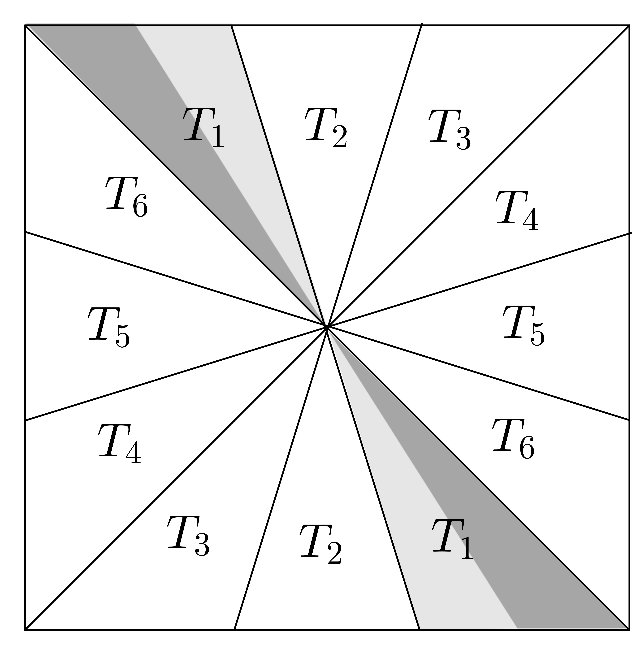
\includegraphics[width = .4\textwidth]{triangle-partition-new.png}
\caption{Partition of frequency square in six directions, where the essential support of $\m{i}$ is contained in each pair of triangles $T_i$. The pair of dark grey triangles is $T_1^-$ and the light grey pair is $T_1^+$.}
\label{fig: partition 2}
\end{figure}
%Let pairs of triangles $T_i$ in Fig.\ref{fig: partition 2} contain the essential support of $\widetilde{m_i},\,i=1,\cdots,6$.
%\eqref{eq: LS-new} takes a similar form to \eqref{eq: LS}, but with $\M\in\mathbb{C}^{8\times 7}$, which is an over-determinant linear system.
In the following, we introduce a triangular partition of frequency square and define formally the concentration of $\widetilde{m_j}$'s support.

\noindent{\bf Definition.}
The {\it essential support} $\Omega_i$ of a function $\widetilde{m_i}$ is the set $\{\V{\omega}:\,|\widetilde{m_i}(\V{\omega})|> |\widetilde{m_j}(\V{\omega})|,\,\forall j\neq i\}$. \vspace{.5em}

Let $T_i$ be pairs of triangles shown in Figure \ref{fig: partition 2}, such that $C_i\subset T_i,\, i = 1,\cdots,6.$ Consider its decomposition, $T_i = T_i^-\bigcup T_i^+$, where $T_i^-, T_i^+$ are halves of $T_i$ adjacent  to $T_{i-1}$ and $T_{i+1}$ respectively.\\[.5em]
\noindent{\bf Definition.}  $\widetilde{m_i}$ {\it concentrates} within $T_i$ if 
\begin{itemize}
\item[(i)] $\Omega_i\subset T_i$;
\item[(ii)]$\text{supp}(\widetilde{m_i})\subset T_{i-1}^+\bigcup T_i\bigcup T_{i+1}^-$ and $\int_\Omega|\widetilde{m_i}| > \int_{\Omega'}|\widetilde{m_i}|, \forall\, \Omega\subset T_i\bigcap\text{supp}(\widetilde{m_i})$, where $\Omega' \subset T_{i-1}^+\bigcup T_{i+1}^-$ is symmetric to $\Omega$ with respect to the boundary of $T_i$.
\end{itemize}

\begin{figure}
\centering
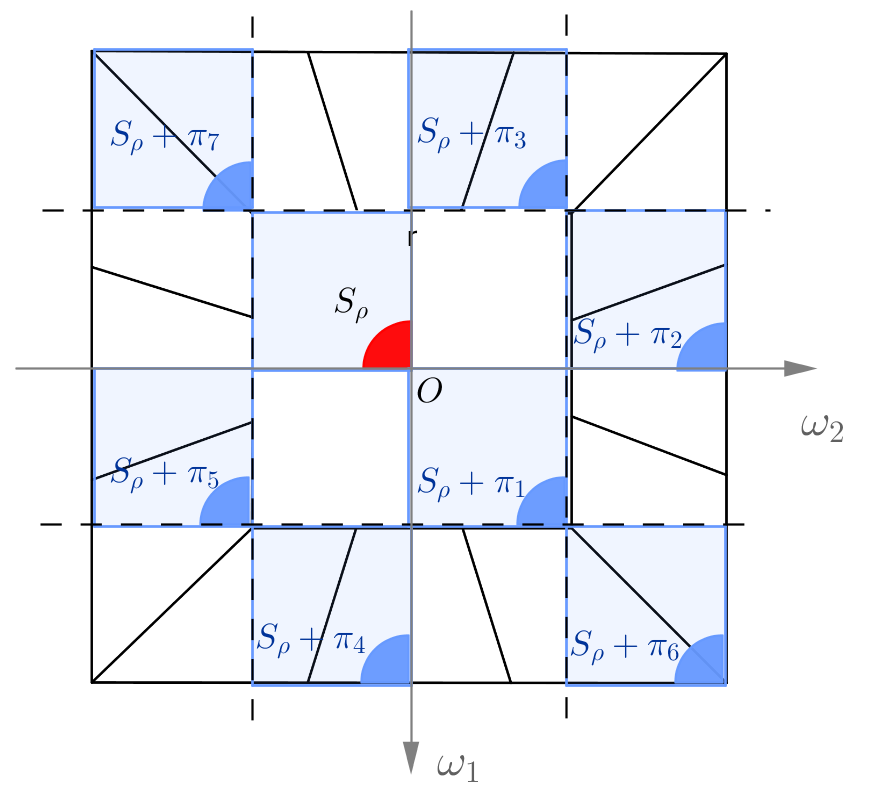
\includegraphics[width = .5\textwidth]{S_shifts2.png}
\caption{$S_{\rho}$ and its shifts}
\label{fig: S-shifts}
\end{figure}
Given $\m{i}$ that concentrates in $T_i$, we study the singularity condition on $\M[-0,:(\V{\omega})],$ specifically in the domain $S_{\rho} = \{(\omega_1,\omega_2)|\;\Vert\omega\Vert < \rho, \omega_1 <0,\,\omega_2<0\}$, see Figure \ref{fig: S-shifts}. 

\begin{lemma}\label{lem: rank1}
$\exists\, \rho>0$ s.t.  if $\M[-0,:](\V{\omega})$ is singular $\forall \V{\omega}\in S_\rho$, then $rank(\mrow{1},\mrow{7})=1$ or $rank(\mrow{3},\mrow{5}) = 1$.
\end{lemma}
Lemma \ref{lem: rank1} can be proved by analyzing the linear dependency and independency between $\mrow{i}$ on $S_\rho$, which have known locations of zero entries when $\rho$ is small due to concentration of $\widetilde{m_j}$.
For the full proof of Lemma \ref{lem: rank1}, see Appendix \ref{app: lemmas}.

Without loss of generality, in the following analysis, we assume $rank(\mrow{1},\mrow{7}) = 1$ on $S_\rho$.
Since only $\mp{1}{1}, \mp{6}{1}$ could be non-zero in $\mrow{1}$ and $\mp{1}{7}, \mp{6}{7}$ could be non-zero in $\mrow{7}$ on $S_\rho$, they are linearly related. Based on this, we can show that $\m{1},\m{6}$ are zero almost everywhere on $S_\rho + \V{\pi}_1$, which implies the discontinuity of $\m{1}$ and $\m{6}$ at $(\frac{\pi}{2},\frac{\pi}{2})$ or $(-\frac{\pi}{2},-\frac{\pi}{2})$.

\begin{proposition}\label{prop: continuity}
$\m{1},\m{6}$ are not continuous at both $(\frac{\pi}{2},\frac{\pi}{2})$ and $(-\frac{\pi}{2},-\frac{\pi}{2})$.
\end{proposition}
\noindent{\it Proof. }
If $\m{1}$ is continuous at $(\frac{\pi}{2},\frac{\pi}{2})$, then $\widetilde{m_1}(\frac{\pi}{2},\frac{\pi}{2}) = \lim_{\alpha\rightarrow 1^-}\widetilde{m_1}(\V{\omega}(\alpha)) = 0$, where $\{\V{\omega}(\alpha),\,0\leq \alpha<1\} \subset S_\rho + \V{\pi}_1$ and $\V{\omega}(1) = (\frac{\pi}{2},\frac{\pi}{2})$. By symmetry, we have $\widetilde{m_6}(\frac{\pi}{2},\frac{\pi}{2}) = 0$. Similarly, the continuity at $(-\frac{\pi}{2},-\frac{\pi}{2})$ implies $\widetilde{m_1}(-\frac{\pi}{2},-\frac{\pi}{2}) = \widetilde{m_6}(-\frac{\pi}{2},-\frac{\pi}{2}) = 0$. Therefore $\mrow{1}(0) = \mrow{7}(0) = \mathbf{0}$ which results in contradiction with Lemma \ref{lem: rank1}.\qed\\[1em]%and from \eqref{eq: m0C} $m_0^C(0)=0$ so that $m_0(0)=0$, %  On the other hand, Proposition\ref{prop: origin-det} implies that $m_0(0) = 0$ as $a = |\widetilde{m_1}(\pi_1)| = 0$, which results in contradiction.
The following theorem summarizes our main result.
\begin{theorem}\label{thm: thm}
If  $\m{i}$ concentrates in $T_i$ and $\m{1},\m{6}$ are symmetric to each other,  then  \eqref{eq: LS-new} doesn't have feasible solution given continuous $\m{1}$ and $\m{6}$.
\end{theorem}

\subsection{Design of input $\m{j}$}\label{sec: phase-design}
In this sub-section, we construct $\m{j},\, j = 1,\cdots,6,$ which concentrate in $T_i$ with high symmetry.
Specifically, following the orthonormal construction in \cite{yin2014orthshear}, we consider $\m{j}$ in the form 
\begin{align}\label{eq: m-form}
\m{j} = e^{-i\V{\eta}_j^\top\V{\omega}}|\m{j}|,\quad j = 1,\cdots,6
\end{align}
 where $|\m{j}|$'s have symmetries with respect to the two diagonals and the two axis. Figure \ref{fig: mjdual} shows such a design of $|\m{j}|$.
 
Given the symmetries of $\m{j}$, for $|m_0(\V{\omega})| > 0,\, \forall\, |\V{\omega}| < \rho$, $\V{\eta}_j$ have to satisfy certain constraints.
% We want to design the phase $\V{\eta}_k$ such that $m_0(\V{\omega}) > 0, \; \forall \omega\in S_1$. This is the same as requiring $\Msub$ to be full rank. We first show the necessary conditions on phases $\V{\eta}$ of the full rank requirement on $\Msub$.
 
\begin{lemma}\label{lem: phase-ineq}
If $\exists\,\V{\omega}\in D_1:=\{\omega_1=\omega_2,\,\omega_1\in(-\frac{\pi}{2},0)\},\,s.t. \,m_0(\V{\omega})>0,$ then $(\V{\eta}_1-\V{\eta}_6)^\top (\V{\pi}_6-\V{\pi}_7)\neq 0(\text{mod}\,2\pi)$. 
\end{lemma} 

Similarly, if $\exists\,\V{\omega}\in \{\omega_1 = \omega_2,\, \omega_1\in(0,\frac{\pi}{2})\},\, s.t.\, m_0(\V{\omega}) > 0$, then $(\V{\eta}_1-\V{\eta}_6)^\top (\V{\pi}_6-\V{\pi}_1)\neq 0(\text{mod}\,2\pi)$. These two conditions are equivalent to 
\begin{align*}
(\V{\eta}_1-\V{\eta}_6)^\top(\pi/2,\pi/2)\neq 0 (\text{mod}\,2\pi)\tag{\bf c1.1}
\end{align*}
given that $\V{\eta}_1$ and $\V{\eta}_6$ are integer phases in $\mathbb{Z}^2$.
Considering the other diagonal segment $\{\omega_2 = -\omega_1, |\omega_1| <\frac{\pi}{2}\}$, we have 
\begin{align*}
(\V{\eta}_3-\V{\eta}_4)^\top(-\pi/2,\pi/2)\neq 0 (\text{mod}\, 2\pi)\tag{\bf c1.2}
\end{align*}
%from the full rank condition.

Next, we investigate $\Msub(\V{\omega})$ at the origin.
\begin{proposition}\label{prop: origin-det}
%If $|\widetilde{m_1}(\V{\pi}_1)| = |\widetilde{m_1}(\V{\pi}_7)| = |\widetilde{m_3}(\V{\pi}_3)| = |\widetilde{m_3}(\V{\pi}_5)|$ and $|\widetilde{m_1}(\V{\pi}_6)|= | \widetilde{m_3}(\V{\pi}_6)|$, then 
If $\widetilde{m_0}(\V{0})\neq 0,$ then $\V{\pi}_1^\top(\V{\eta}_1-\V{\eta}_6)\neq \pi(\text{mod}\,2\pi)$ or $\V{\pi}_3^\top(\V{\eta}_3-\V{\eta}_4)\neq \pi(\text{mod}\,2\pi)$. 
\end{proposition}

\begin{comment}
{\it Remark.} In Lemma \ref{lem: phase-ineq}, $\Msub[:,1]$ and $\Msub[:,6]$ being independent only guarantees $\det(\Msub[-k_{\V{\omega}},:])\neq 0$. However, \eqref{eq: m0-cramer} implies that $|m_0(\V{\omega})|\propto \det(\Msub[-k_{\V{\omega}},:])$ hence it is preferred to maximize the determinant. Since
\begin{align*}
\det(\Msub[-k_{\V{\omega}}, :]) = \det\big(\big[\, \Msub[-k_{\V{\omega}},-6], \;\Msub[-k_{\V{\omega}},6] + c \cdot\Msub[-k_{\V{\omega}},1]  \,\big]\big),\quad 
\end{align*}
$\forall c\in \mathbb{C}$, the angle between $\Msub[:,1]$ and $\Msub[:,6]$ should be maximized.
Therefore, a stronger condition than ({\bf c1.1}) is to require $\Msub[:,1]$ and $\Msub[:,6]$ be orthogonal, which is equivalent to 
\begin{align*}
(\V{\eta}_1-\V{\eta}_6)^\top(\pi/2, \pi/2) = \pi \,(\text{mod}\, 2\pi).\tag{\bf c2.1}
\end{align*}
The stronger condition corresponding to ({\bf c1.2}) is 
\begin{align*}
(\V{\eta}_3-\V{\eta}_4)^\top(-\pi/2,\pi/2)=\pi(\text{mod},\,2\pi).\tag{\bf c2.2}
\end{align*} %from the stronger orthogonal condition.

%{\it Remark}
%f $|\m{1}| = |\m{2}|$ on $\{\omega_y = 3\omega_x,\,|\omega_x| > \frac{\pi}{2}\}$ and $m_0(\V{\omega}) > 0$ on $\{\omega_y = 3\omega_x\pm \pi,\,|\omega_y| <\frac{\pi}{2}\}$, then the same conditions ({\bf c1}) and ({\bf c2}) can be derived from full rank and orthogonal conditions respectively for tuples $(\,\V{\eta}_1,\,\V{\eta}_2,(-\pi/2,\pi/2)\,),\,(\,\V{\eta}_2,\V{\eta}_3,(\pi/2,\pi/2)\,),\,(\V{\eta}_4,\V{\eta}_5,\,(\pi/2,\pi/2)\,)$ and $(\,\V{\eta}_5,\V{\eta}_6,\,(-\pi/2,\pi/2)\,)$. 

% If the previous strong orthogonal condition on $\V{\eta}_1, \V{\eta}_3, \V{\eta}_4,\V{\eta}_6$ holds, then $K_1 = K_2 = 0$ and $m_0(0)=m_0^C(0)= 0$. Therefore, the strong orthogonal conditions ({\bf c2}) cannot be satisfied at the same time. 
%In particular, we consider the following constraints on phase $\V{\eta}_k\in \mathbb{Z}^2,\, k = 1,\cdots,6$:
Unfortunately, Proposition \ref{prop: origin-det} prevents ({\bf c2.1}) and ({\bf c2.2}) from holding simultaneously.
\end{comment}
We propose the following set of phases that satisfy the necessary conditions in Lemma \ref{lem: phase-ineq} and Proposition \ref{prop: origin-det},
\begin{align}\label{eq: phase-sol}
\V{\eta}_1 = (0,0),\; \V{\eta}_2 = (-1,1),\; \V{\eta}_3 = (0,2),\notag\\
\V{\eta}_4 = (1,0),\; \V{\eta}_5 = (0,-1),\; \V{\eta}_6 = (0,1).
\end{align}
\begin{comment}
where
\begin{align*}
%\label{eq: phase-constraint}
%&(\V{\eta}_1-\V{\eta}_2)^\top(-\pi/2, \pi/2) = (\V{\eta}_5-\V{\eta}_6)^\top(-\pi/2,\pi/2) = \pi\, (\text{mod}\, 2\pi)\notag\\
%&(\V{\eta}_2-\V{\eta}_3)^\top(\pi/2,\pi/2) = (\V{\eta}_4-\V{\eta}_5)^\top(\pi/2,\pi/2) = \pi\, (\text{mod}\, 2\pi)\\
%&
(\V{\eta}_3-\V{\eta}_4)^\top(-\pi/2, \pi/2) &=-\pi/2\,(\text{mod}\,2\pi)\notag\\
 (\V{\eta}_6 - \V{\eta}_1)^\top(\pi/2,\pi/2) &= \pi/2\, (\text{mod}\,2\pi)\notag
\end{align*}
%where we require strong orthogonal constraints on pair of shifts corresponding to $\widetilde{m}$ function with non-diagonal common boundary and weaker constraints on $(\V{\eta}_1,\V{\eta}_6)$ and $(\V{\eta}_3,\V{\eta}_4)$. A solution to \eqref{eq: phase-constraint} is 
\end{comment}

\subsection{Solving \eqref{eq: LS-new} and \eqref{eq: identity-cond} for $m_0,\widetilde{m_0}$ and $m_j$}\label{subsec: compute-m0}
Once $\m{j}, j= 1,\cdots, 6$ are fixed, \eqref{eq: LS-new} can be reformulated as follows,
\begin{align}\label{eq: mj-eq}
\M[:,-0](\V{\omega}) 
\begin{bmatrix}
m_1(\V{\omega})\\
m_2(\V{\omega})\\
m_3(\V{\omega})\\
m_4(\V{\omega})\\
m_5(\V{\omega})\\
m_6(\V{\omega})
\end{bmatrix}
= \V{b}_0 - m_0(\V{\omega})
\begin{bmatrix}
 \overline{\widetilde{m_0}}(\V{\omega})\\
 0\\
\sbarmp{0}{2}\\
0\\
\sbarmp{0}{4}\\
0\\
\sbarmp{0}{6}\\
0
\end{bmatrix} \doteq \V{b}_0'(\V{\omega}),
\end{align}
where $\M[:,-0]$ is determined by $\m{j},\,j = 1,\cdots,6$ 
and $m_j,\,j=1,\cdots,6$ can be uniquely solved if and only if
\hspace{-1em}
\begin{enumerate}[leftmargin=.5in]
\item[\mylabel{cond: i}{(\ref{subsec: compute-m0}.i)}] $\M[:,-0]$ is full rank,%
\item[\mylabel{cond: ii}{(\ref{subsec: compute-m0}.ii)}] $\V{b}_0'(\V{\omega})$ is in $col\big(\M[:,-0](\V{\omega})\big)$, the column space of $\M[:,-0]$.%
\end{enumerate}
%Because , \ref{cond: i} can be easily checked by computing $\det(\M[:,-0]^\top\M[:,-0])$ and see if it is non-zero. Next, we show that (ii) provides an explicit way of computing $m_0(\V{\omega})$ without knowing $\m{0}$.
Next, we show that \ref{cond: ii} breaks down to constraints on two submatrices of $\M[:,-0]$ and quadruple $\big( m_0(\V{\omega}),m_0(\V{\omega}+\V{\pi}_2), m_0(\V{\omega} +\V{\pi}_4), m_0(\V{\omega}+\V{\pi}_6) \big)$.
\begin{proposition}\label{prop: m0_formula}
Let $\M[odd,-0],\M[even,-0]\in\mathbb{C}^{4\times6}$ be the sub-matrices of $\M[:,-0]$ consisting of odd and even rows respectively. Suppose {\rm\ref{cond: i}} holds, then {\rm\ref{cond: ii}} holds if and only if $rank(\M[odd,-0]) = rank(\M[even,-0]) = 3$ and 
\begin{align}\label{eq: m0-even-null}
[m_0(\V{\omega}),m_0(\V{\omega}+\V{\pi}_2), m_0(\V{\omega} +\V{\pi}_4), m_0(\V{\omega}+\V{\pi}_6)]\, \M[even,-0](\V{\omega}) = \V{0},
\end{align}
\begin{align}\label{eq: m0-odd-null}
[m_0(\V{\omega}+\V{\pi}_1),m_0(\V{\omega}+\V{\pi}_3), m_0(\V{\omega} +\V{\pi}_5), m_0(\V{\omega}+\V{\pi}_7)] \,\M[odd,-0](\V{\omega}) = \V{0}.
\end{align}
\end{proposition}
\noindent{\it Remark.} Both conditions \eqref{eq: m0-even-null} and \eqref{eq: m0-odd-null} hold $\forall \V{\omega}\in[-\pi,\pi)\times[-\pi,\pi)$ if and only if \eqref{eq: m0-even-null} holds $\forall \V{\omega}\in [-\pi,0)\times[-\pi,0)$.

According to Proposition \ref{prop: m0_formula}, $\M[:,-0]$ (or equivalently $\widetilde{m_j}$) has to satisfy the following rank constraints for \eqref{eq: mj-eq} to be uniquely solvable, 
\begin{align}\label{eq: Mranks}
rank(\M[:,-0]) = 6,\, rank(\M[odd,-0]) = rank(\M[even,-0]) = 3.
\end{align}
Furthermore, given \eqref{eq: Mranks} holds, the quadruple  $\big( m_0(\V{\omega}),m_0(\V{\omega}+\V{\pi}_2), m_0(\V{\omega} +\V{\pi}_4), m_0(\V{\omega}+\V{\pi}_6) \big)$ can be solved by \eqref{eq: m0-even-null} upto a non-zero constant $c(\V{\omega})$. The next proposition shows that this is sufficient to obtain a feasible $m_0(\V{\omega})$.

\begin{comment}
By Lemma \ref{lem: M-symmetry}, $\M[:,-0]$ are the same at $\V{\omega},\V{\omega}+\V{\pi}_2,\V{\omega}+\V{\pi}_4$ and $\V{\omega} + \V{\pi}_6$ up to row permutations. Therefore, the columns of the matrix $\V{B}$ below should be in $col\big(\M[:,-0](\V{\omega})\big)$,
\begin{align*}
\V{B}&= \widetilde{\mathbf{m}_0}^\uparrow\otimes\mathbf{m}_0 - [\V{b}_0,\V{b}_2,\V{b}_4,\V{b}_6]\\
&\doteq
\begin{bmatrix}
 \overline{\widetilde{m_0}}(\V{\omega})\\
 0\\
\sbarmp{0}{2}\\
0\\
\sbarmp{0}{4}\\
0\\
\sbarmp{0}{6}\\
0
\end{bmatrix}
\otimes
\begin{bmatrix}
 m_0(\V{\omega})\\
 m_0(\V{\omega} + \V{\pi}_2)\\
 m_0(\V{\omega} + \V{\pi}_4)\\
 m_0(\V{\omega} + \V{\pi}_6) 
\end{bmatrix}
-
\begin{bmatrix}
1 & 0 & 0 & 0\\
0 & 0 & 0 & 0\\
0 & 1 & 0 & 0\\
0 & 0 & 0 & 0\\
0 & 0 & 1 & 0\\
0 & 0 & 0 & 0\\
0 & 0 & 0 & 1\\
0 & 0 & 0 & 0
\end{bmatrix},
\end{align*}

Let $\M[:,-0] = U\Sigma V^\top$ be the singular value decomposition of $\M[:,-0]$, such that $U(\V{\omega})\in\mathbb{C}^{8\times 6}$ consists of left singular vectors of $\M[:,-0](\V{\omega})$ and $UU^\top(\V{\omega})$ is a projection matrix of $col\big(\M[:,-0](\V{\omega})\big)$. Therefore, $\V{B}$ satisfies
\begin{align}\label{eq: cond-full}
\V{P}\V{B} = (\V{U}\V{U}^\top - \V{I}_8 )\V{B} = \V{0}\in\mathbb{C}^8,
\end{align}
 where $\V{P}$ is the projection onto $col\big(\M[:,-0](\V{\omega})\big)^\bot$, $\V{I}_8$ is the identity matrix in $\mathbb{C}^8$. Because the even rows of $\V{B}$ are all zeros, we can down-sample its rows and correspondingly the columns of $\V{P}$ and \eqref{eq: cond-full} can be reduced to 
\begin{align}
\V{P}^\downarrow\V{B}^\downarrow = \V{P}^\downarrow \big(\widetilde{\mathbf{m}_0}\otimes \mathbf{m}_0 - \V{I}_4\big) = \V{0}\in\mathbb{C}^8
\end{align}
$\V{P}^\downarrow\in\mathbb{C}^{8\times 4}$ consists of odd columns of $\V{P}$ and $\V{B}^\downarrow\in\mathbb{C}^{4\times 4}$ consists of odd rows of $\V{B}$.

Let $C_{\V{\omega}} = det(\M[-k_{\V{\omega}},:])$, then we have the following observation.
\begin{lemma}\label{lem: equal-det}
$C_{\V{\omega}} = C_{\V{\omega}+\V{\pi}_2} = C_{\V{\omega}+\V{\pi}_4} = C_{\V{\omega}+\V{\pi}_6}$
\end{lemma}
\noindent{\it Proof}
Because $\widetilde{M}(\V{\omega}+\V{\pi}_2) = P_{\V{\pi}_2}\M(\V{\omega})$ where $P_{\V{\pi}_2}$ is a row permutation matrix, it follows from the definition of $C_{\V{\omega}}$ that 
$C_{\V{\omega}} = det\big(\M[-k_{\V{\omega}},:](\V{\omega})\big) = det\big(\M[-k_{\V{\omega}+\V{\pi}_2},:](\V{\omega}+\V{\pi}_2) \big)= C_{\V{\omega}+\V{\pi}_2}$ where 
$\mathbf{1}_{k_{\V{\omega}+\V{\pi}_2}} = P_{\V{\pi}_2}\mathbf{1}_{k_{\V{\omega}}}$.
\qed\\[1em]
We assume that $m_0\in\mathbb{R}_{\geq 0}$ without phase. Let $m_0^C(\V{\omega}) = m_0(\V{\omega})|C_{\V{\omega}}|\in \mathbb{R}_{\geq 0}$ and $\mc{0} = \m{0}/|C_{\V{\omega}}|$, then Lemma \ref{lem: equal-det} implies the following.
\end{comment}


\begin{proposition}\label{prop: mc}
If $\m{j}, m_j(\V{\omega}),\,  j = 0,1,...,6$ satisfy \eqref{eq: LS-new} and \eqref{eq: identity-cond}, 
%$m_0^C(\V{\omega}),$ $\,\mc{0}, m_i(\V{\omega}),\,i = 1,...,6$ do. More generally, 
%$m_0(\V{\omega})c(\V{\omega}),\,\m{0}c(\V{\omega})^{-1}, m_i(\V{\omega}),\,i=1,...,6$ 
$m_0^c(\V{\omega})\doteq m_0(\V{\omega})c(\V{\omega}), \widetilde{m_0}^c(\V{\omega})\doteq \m{0}\overline{c}(\V{\omega})^{-1}$ and $m_j(\V{\omega}),\m{j}, \, j = 1,\cdots,6$ 
satisfy \eqref{eq: LS-new} and \eqref{eq: identity-cond} if $ c(\V{\omega}) = c(\V{\omega}+\V{\pi}_2)=c(\V{\omega}+\V{\pi}_4) = c(\V{\omega}+\V{\pi}_6) \neq 0$, i.e. $c(\V{\omega})$ is $\pi$-periodic in both $\omega_1$ and $\omega_2$.
\end{proposition}
\noindent{\it Proof. }
It suffices to show that $m_0^c(\V{\omega})\overline{\widetilde{m_0}^c}(\V{\omega} + \V{\pi}_i) = m_0(\V{\omega})\sbarmp{0}{i},\,$ when $i$ is even.\qed

%\begin{align*}
%m_0^c(\V{\omega})\overline{\widetilde{m_0}^c}(\V{\omega} + \V{\pi}_i) = m_0(\V{\omega})\sbarmp{0}{i},\quad & i \text{ is even,}\hspace{4em}\qed
%\hspace{1em}m_j^c(\V{\omega})\overline{\widetilde{m_j}^c}(\V{\omega} + \V{\pi}_i) = \big(m_j(\V{\omega})\sbarmp{j}{i}\big)c(\V{\omega})c(\V{\omega}+\V{\pi}_1)^{-1},\quad & i \text{ is odd.}\qedhere\hspace{2em}\qed
%\end{align*}

Next, we solve quadruple $(\m{0}, \mp{0}{2}, \mp{0}{4}, \mp{0}{6})$ from the identity condition \eqref{eq: identity-cond} on $[-\pi, 0)\times[-\pi, 0 )$. We reformulate it as a quadratic optimization problem that minimizes the total variation of $\sbarm{0}m_0(\V{\omega})$ as follows,
%On a $2N\times 2N$ grid $\G$ of $S_0 = [-\pi, \pi)\times[-\pi, \pi)$, s.t. $\forall \V{\omega}_j \in \G, \; \V{\omega}_j+\V{\nu}_1,\,\V{\omega}_j+\V{\nu}_2,\,\V{\omega}_j+\V{\nu}_3 \in \G$, \eqref{eq: m0-sol} is reformulated as
\begin{align}\label{eq: opt}
\min_{\xvec}\; \Vert \V{D}(\mathbf{m}_0\circ\xvec)\Vert^2,\quad 
s.t. \; \V{A}\xvec = \mathbf{1},
\end{align}
where $\V{D}$ is the gradient operator, $\circ$ is Hadamard product and $\V{A}$ is the linear operator from \eqref{eq: identity-cond}. In particular, on a $2N\times 2N$ regular grid $\G=\{\V{\omega}_i\}_{i=1}^{4N^2}$ of $[-\pi, \pi)\times[-\pi, \pi), $ \eqref{eq: identity-cond} can be rewrite as
\begin{align}
\V{A}\, \overline{\widetilde{\mathbf{m}_0}}= \mathbf{1}_{4N^2}, \label{eq: m0-A}%\\ 
%\widetilde{\mathbf{m}_0} = [\widetilde{m_0}(\V{\omega}_i)]_{\,i=1,\hdots,4N^2}&\in\mathbb{C}^{4N^2} \notag
\end{align}
where $\widetilde{\mathbf{m}_0} = [\widetilde{m_0}(\V{\omega}_i)]_{\,i=1}^{4N^2}$ and $\V{A}\in \mathbb{C}^{N^2\times 4N^2}$ is a sparse matrix with entries 
$$\V{A}_{i,j} = m_0(\V{\omega}_j)\sum_{k=0}^3\delta(\V{\omega}_j-\V{\omega}_i-\V{\pi}_{2k}), \quad \V{\omega}_j \in [-\pi,0)\times[-\pi,0).$$
%Because the set $\{\V{\omega},\, \V{\omega}+\V{\nu}_k,k=1,2,3\}$ is invariant under the shift $\V{\nu}_i,\, i = 1,2,3,$ the rows of $\V{A}$ corresponding to $\V{\omega}$ and $\V{\omega}+\V{\nu}_i$ are identical and 
%Because we only need to consider \eqref{eq: identity-cond} on $[-\pi,0)\times[-\pi,0)$, 
%rows corresponds to $\V{\omega}\in [-\pi,\pi)\times[-\pi,\pi)/\{\V{0},\,\V{\nu}_i,i=1,2,3\}$. Therefore, after removing the duplicate rows, 
%$\V{A}\in \mathbb{C}^{N^2\times 4N^2}$ and \eqref{eq: m0-A} is under-determinant. \\
%We thus use \eqref{eq: m0-A} as a linear constraint in quadratic optimization to solve $\mathbf{\widetilde{m}_0}$. Suppose that $\m{0}$ is smooth, then we build a differential operator $\V{D}$ and solve the following minimization problem:
%or
%\begin{align}
%&\min_{\mvec{0}}\; \Vert \V{D}\mvec{0}\Vert^2 + \lambda \Vert \V{A}\mvec{0} - \mathbf{1}\Vert^2 \label{eq: m0-smooth-relaxed}
%\end{align}
%The solution of \eqref{eq: m0-smooth-relaxed} is $\mvec{0} = \lambda(\lambda \V{A}^\top \V{A} + \V{D}^\top \V{D})^{-1}\V{A}^\top\mathbf{1}$.

%Or suppose $\m{0}$ decays away from the origin, then we build a diagonal weighting operator $\V{W}$, and solve the following minimization problem:
%\begin{align}\label{eq: opt-weight}
%&\min_{\mvec{0}}\; \Vert \V{W}\mvec{0}\Vert^2,\quad s.t. \; \V{A}\mvec{0} = \mathbf{1}
%\end{align}
Supplementary numerical results on solving $\m{0}$ by optimization are provided in Appendix \ref{app: supp-numerical}, where we test this optimization method on known bi-orthogonal filters $m_0$ and $\widetilde{m_0}$ and compare the solution from the optimization with the ground truth.

Finally, we plug $m_0(\V{\omega})$ and $\m{0}$ into $\V{b}_0'(\V{\omega})$ on the right of \eqref{eq: mj-eq} and solve the linear system, which has a guaranteed unique solution.

%According to Proposition \ref{prop: mc}, we can first solve $\mc{0}$ and $m_0^C(\V{\omega})$ and then construct $c(\V{\omega})$ for optimal $\m{0}$ and $m_0(\V{\omega})$. 
%In particular, $m_0^C$ can be computed without knowing $k_{\V{\omega}}$,
%\begin{align}\label{eq: m0C}
%m_0^C(\V{\omega}) = m_0(\V{\omega})|C_{\V{\omega}}| = |det(\M_{1,1}[-k_{\V{\omega}},:])| = \prod_{i=1}^6\sigma_i(\M_{1,1}[-k_{\V{\omega}},:]) = \prod_{i=1}^6\sigma_i(\M_{1,1}).
%\end{align}
%In practice, we first perform QR decomposition on $\Msub:=\M_{1,1}$ and then take the absolute value of the product of the diagonal entries of the upper triangular matrix, $diag(R)$. 
To sum up, we propose the following algorithm for bi-orthogonal directional filter construction with dilated quincunx downsampling scheme:\\
\rule{\textwidth}{.5pt}
\begin{description}% prevent items from splitting
\item[construction of $m$-, $\widetilde{m}$-functions in bi-orthogonal basis]\
\begin{itemize}
\item[Input:] $\m{j},\,j=1,...,6$
\item[step 1.] construct $\M[:,-0](\V{\omega})$ on sub-grid $[-\pi,0)\times[-\pi,0)$ and check rank constraints \eqref{eq: Mranks}.%compute $m_0^C(\V{\omega}) = \left|det(\M_{1,1}[-k_{\V{\omega}},:])\right|$
\item[step 2.] solve quadruple $\big( m_0(\V{\omega}),m_0(\V{\omega}+\V{\pi}_2), m_0(\V{\omega} +\V{\pi}_4), m_0(\V{\omega}+\V{\pi}_6) \big)$ using \eqref{eq: m0-even-null} on $[-\pi,0)\times[-\pi,0)$,%compute $\mc{0}$, such that \eqref{eq: LS-new} is solvable and \eqref{eq: identity-cond} holds
\item[step 3.] solve the optimization \eqref{eq: opt} for $\m{0}$ on grid $[-\pi,\pi)\times[-\pi,\pi)$.
%solve $m_i(\V{\omega}),\, i=1,...,6$ according to \eqref{eq: LS-new}
\item[step 4.] solve the reduced linear system \eqref{eq: mj-eq} for $m_j(\V{\omega}),\, j = 1,\cdots,6$.%design $c(\V{\omega})$ and let $m_0(\V{\omega}) = m_0^C(\V{\omega})c(\V{\omega}),\,\m{0} = \mc{0}\overline{c}(\V{\omega})^{-1}$
\end{itemize}
\end{description}
\rule{\textwidth}{.5pt}\\[.5em]

Proposition \ref{prop: mc} suggests that we can design $c(\V{\omega})$ such that $(m_0^c,\widetilde{m_0}^c)$ have desired properties, e.g. continuity, smoothness or fast decay rate. In practice, we compute $m_0(\V{\omega})\sbarm{0}$ from $m_0(\V{\omega})$ and $\m{0}$ obtained in step 2 and 3, then re-decompose the product into $m_0^c(\V{\omega})$ and $\overline{\widetilde{m_0}^c}(\V{\omega})$.

We may also manipulate pairs of $(m_j,\widetilde{m_j})$ in a similar way due to the following generalization of Proposition \ref{prop: mc}.
\begin{proposition}\label{prop: mjc}
If $\m{j}, m_j(\V{\omega}),\,  j = 0,1,...,6$ satisfy \eqref{eq: LS-new} and \eqref{eq: identity-cond}, 
$m_j^c(\V{\omega})\doteq m_j(\V{\omega})c_j(\V{\omega}), \widetilde{m_j}^c_j(\V{\omega})\doteq \m{j}\overline{c}(\V{\omega})^{-1} \, j = 0,\cdots,6$ 
satisfy \eqref{eq: LS-new} and \eqref{eq: identity-cond} if $ c_0(\V{\omega}) = c_0(\V{\omega}+\V{\pi}_{2k})\,,\forall k = 0,\cdots,3$ and $c_j(\V{\omega}) = c_j(\V{\omega} + \V{\pi}_k),\, \forall \;k = 0,\cdots,7,\, j = 1,\cdots,6$.
\end{proposition}

\begin{comment}
\subsection{solving $m_i$}
In the final step, we substitute $\mc{0}$ and $m_0^C(\V{\omega})$ into \eqref{eq: LS-new} and rewrite it into the following linear system,
\begin{align}\label{eq: mi}
\overline{\M}[:,2:7]\,\mathbf{m}[2:7](\V{\omega}) = 
\begin{bmatrix}
1-m_0^C\overline{\widetilde{m_0}^C}(\V{\omega})\\
0\\
-m_0^C\overline{\widetilde{m_0}^C}(\V{\omega}+\V{\pi}_2)\\
\vdots \\
0
\end{bmatrix}
=:\mathbf{b}(\V{\omega}).
\end{align}
The solution of \eqref{eq: mi} depends only on $m_0^C\overline{\widetilde{m_0}^C}$, or equivalently $m_0\overline{\widetilde{m_0}}$. 
\end{comment}

\section{Numerical Experiments}

In this section, we show an example of the numerical construction of biorthogonal directional wavelets on a quincunx lattice using our proposed algorithm in Matlab.

We design $\widetilde{m_j}$ in the form of \eqref{eq: m-form}, using phases in \eqref{eq: phase-sol} and amplitudes $|\widetilde{m_j}|$ shown in Figure \ref{fig: mjdual}. For the construction of $|\widetilde{m_j}|$, we start with $|\widetilde{m_2}|$, then compute $|\widetilde{m_1}|$ and $|\widetilde{m_3}|$ by shearing $|\widetilde{m_2}|$ counter-clockwise and clockwise respectively. $|\widetilde{m_4}|, |\widetilde{m_5}|$ and $|\widetilde{m_6}|$ are obtained by symmetry along the diagonal. This is the same approach used in the shearlet construction \cite{kutyniok2012digital}. Furthermore, $\m{j} = 0,\,\forall \V{\omega}\in C_0 = [-\frac{\pi}{2},\frac{\pi}{2})\times [-\frac{\pi}{2},\frac{\pi}{2}).$ In particular, by Proposition \ref{prop: continuity}, we enforce $|\widetilde{m_1}(\frac{\pi}{2},\frac{\pi}{2})|\neq 0$ and $\widetilde{m_6}(\frac{\pi}{2},\frac{\pi}{2})|\neq 0$.

Using these $\m{j},\,j = 1,\cdots,6$ as input, the main algorithm in Section \ref{subsec: compute-m0} yields $m_0,\widetilde{m_0}$ and $m_j, \, j = 1,\cdots, 6$. As the first step, we numerically check that this particular design of $\widetilde{m_j}$ satisfies the rank constraints \eqref{eq: Mranks}. As shown in Figure \ref{fig: m_0} $m_0(\V{\omega})$ obtained in step 2 is supported on the central square $C_0$, where $|m_0(\V{\omega})| = 1$. Moreover, Figure \ref{fig: m_0_m0dual} shows that $\m{0} = \overline{m_0^{-1}}(\V{\omega}) = m_0(\V{\omega})$ on $C_0$, i.e. $\m{0}$ solved in step 3 is numerically the same as $m_0(\V{\omega})$.
Figure \ref{fig: m_j} and Figure \ref{fig: m_j_mjdual} show $|\m{j}|$ and $|m_j\m{j}|$ for $\m{j}$ obtained by solving \eqref{eq: mj-eq}. We also numerically check that $m_j(\V{\omega})$ and $\m{j}$ have the same phase, i.e. $m_j\m{j}\in \mathbb{R}$.

So far, we construct a set of $(m_j,\widetilde{m_j})_{j = 0,\cdots,6}$ that satisfies \eqref{eq: LS-new} and \eqref{eq: identity-cond}, thus it can be used to construct biorthogonal wavelets based on \eqref{eq: mj} and \eqref{eq: mj_dual}. However, $m_0$ and $\widetilde{m_0}$ here are not continuous. To improve the regularity of the corresponding wavelets, by Proposition \ref{prop: mc} and the observation $m_0\sbarm{0} = \V{1}_{C_0}$, we replace $(m_0,\widetilde{m_0})$ by $(m_0', \widetilde{m_0}')$, where $\widetilde{m_0}'$ is a smooth real function supported on $C_0$ and $m_0'(\V{\omega}) = \V{1}_{C_0}(\overline{\widetilde{m_0}'})^{-1}(\V{\omega})$. Figure \ref{fig: smooth_m0dual} shows such a pair of $(m_0',\widetilde{m_0}')$. Finally, using pre-designed $\m{j}$ and post-designed $\widetilde{m_0}'$, we construct the dual wavelets  $\widetilde{\psi^j}$ in \eqref{eq: bi-orth MRA} using \eqref{eq: mj_dual}. As shown in Figure \ref{fig: wavelets}, the dual wavelets are spatially localized and have good direction selection. The wavelets and scaling functions in \eqref{eq: bi-orth MRA} can be constructed using \eqref{eq: mj_dual} similarly.

\begin{figure}
\centering
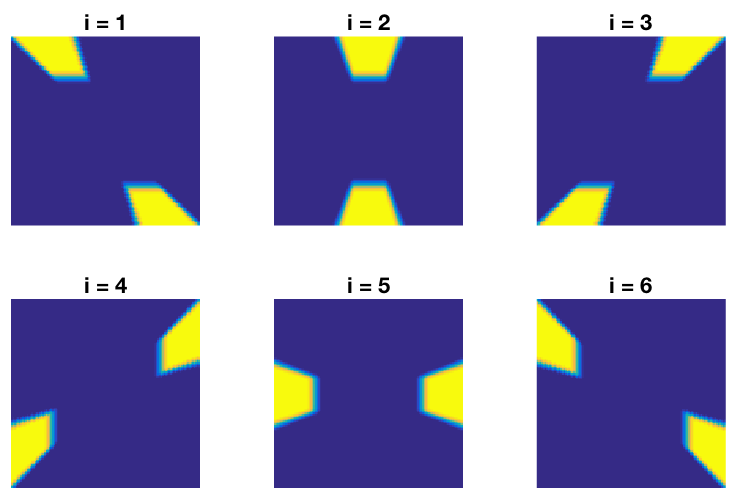
\includegraphics[width=.8\textwidth]{initialize_mdual.png}
\caption{ Input $|\m{j}|$ constructed in the same way as shearlets.}
\label{fig: mjdual}
\end{figure}

\begin{figure}
\centering
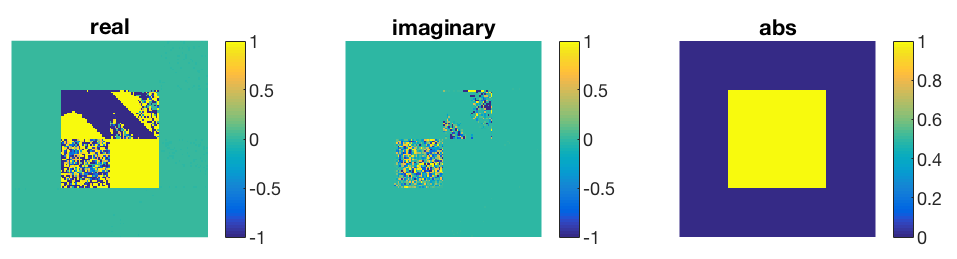
\includegraphics[width=\textwidth]{m0.png}
\caption{ $m_0(\V{\omega})$ constructed from $\widetilde{m_j}$. Left to right: $Re(m_0(\V{\omega})),\, Im(m_0(\V{\omega}))$ and $|m_0(\V{\omega})|$.}
\label{fig: m_0}
\end{figure}

\begin{figure}
\centering
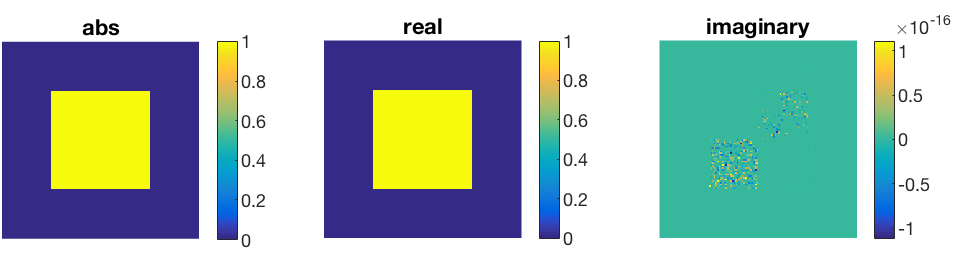
\includegraphics[width=\textwidth]{m0_m0dual_new.png}
\caption{$|\m{0}|$ and $m_0\sbarm{0}$, where $\m{0}$ is solved by optimization \eqref{eq: opt}, given $\widetilde{m_j}$ in Figure \ref{fig: mjdual} and $m_0$ in Figure \ref{fig: m_0}. Left to right: $|\m{0}|$, $Re(m_0\sbarm{0})$ and $Im(m_0\sbarm{0})$. }
\label{fig: m_0_m0dual}
\end{figure}

\begin{figure}
\centering
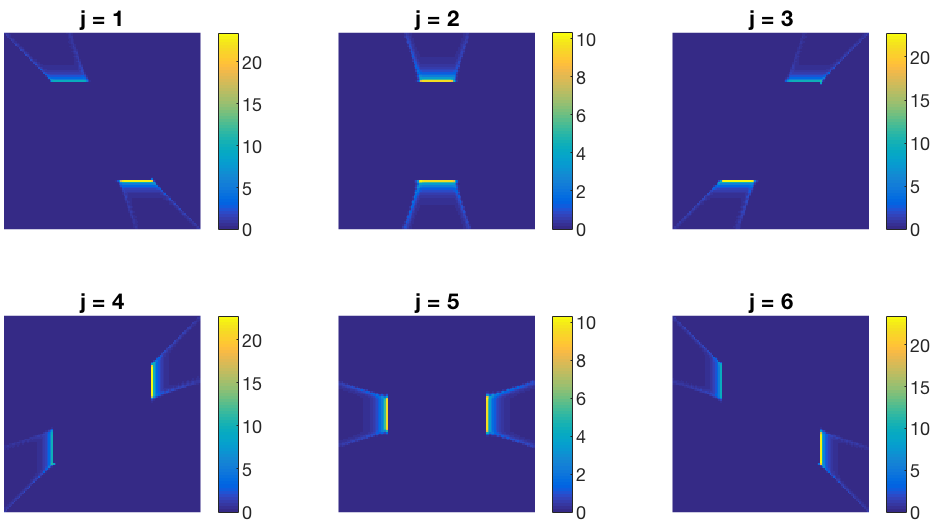
\includegraphics[width=\textwidth]{m.png}
\caption{ $|m_j(\V{\omega})|$, where $m_j(\V{\omega})$ is solved from \eqref{eq: mj-eq} given $\widetilde{m_j}$ in Figure \ref{fig: mjdual}, $m_0$ in Figure \ref{fig: m_0} and $\widetilde{m_0}$ in Figure \ref{fig: m_0_m0dual}. }
\label{fig: m_j}
\end{figure}

\begin{figure}
\centering
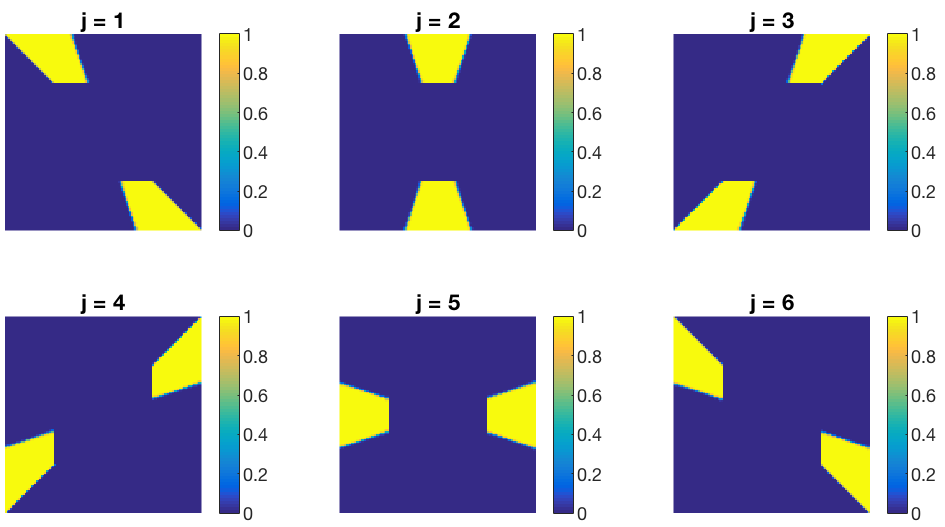
\includegraphics[width=\textwidth]{m_mdual.png}
\caption{ $|m_j(\V{\omega})\m{j}|$ }
\label{fig: m_j_mjdual}
\end{figure}

\begin{figure}
\centering
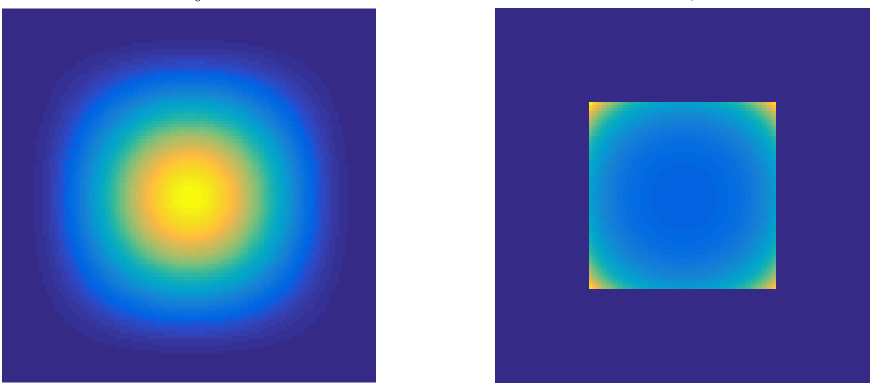
\includegraphics[width=.66\textwidth]{smooth_m0dual.png}
\caption{ Left: $\widetilde{m_0}'$, designed smooth function mainly supported on the central square $C_0$, right: $m_0'$, $s.t. m_0'\overline{\widetilde{m_0}'}(\V{\omega})  =  m_0\overline{\widetilde{m_0}}(\V{\omega})= \V{1}_{C_0}(\V{\omega})$. } 
\label{fig: smooth_m0dual}
\end{figure}

\begin{figure}
\centering
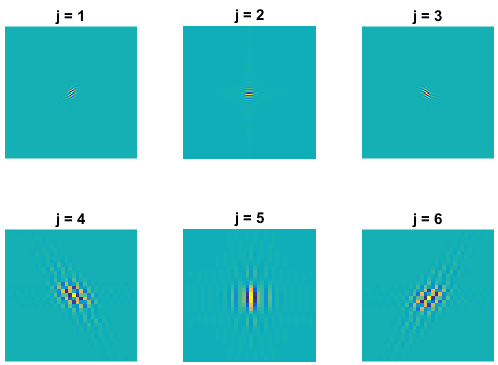
\includegraphics[width=.8\textwidth]{quincunx_wavelets.png}
\caption{ Real part of $\psi^j$ constructed from $\widetilde{m_0}'$ in Figure \ref{fig: smooth_m0dual} and $\widetilde{m_j},\, j=1,\cdots, 6$ in Figure \ref{fig: mjdual} using \eqref{eq: mj_dual}. Top: $\widetilde{\psi^j}$ without scaling, bottom: $\widetilde{\psi^j}$ with eight time zoom-in } 
\label{fig: wavelets}
\end{figure}


\begin{comment}
\subsection{solving $m_0^C$}
A set of $\m{i}$ that satisfy the conditions of Theorem \ref{thm: thm} with phase terms in \eqref{eq: phase-sol} is used as the input of \eqref{eq: LS-new}.
The left figure in Fig.\ref{fig: tm_i_m_0} shows the absolute value of $\m{i}$. In particular, $\m{i} =0,\,\forall \omega\in S_1$. 
We follow the construction process in Section \ref{subsec: compute-m0} and obtain $m_0^C$ shown in the right of Fig.\ref{fig: tm_i_m_0}, in both normal scale and log scale.  
We perform a numerical sanity check on the necessary condition in Proposition \ref{prop: feasibility}, that is $\forall\,\V{\omega}, \,s.t. [m_0(\V{\omega}), m_0(\V{\omega}+\V{\pi}_2),m_0(\V{\omega}+\V{\pi}_4),m_0(\V{\omega}+\V{\pi}_6)]$ is not a linear combination of the rows of $\mathfrak{D}(\V{\omega})$ in \eqref{eq: singular-cond}. Equivalently, we compute the following quantity $$\vartheta = 1 - \Vert V^\top\mathfrak{m}_0 \Vert/\Vert \mathfrak{m}_0\Vert ,$$ where $\mathfrak{m}_0(\V{\omega})=[m_0(\V{\omega}), m_0(\V{\omega}+\V{\pi}_2),m_0(\V{\omega}+\V{\pi}_4),m_0(\V{\omega}+\V{\pi}_6)]^\top$ and $V$ are the left singular vectors of $\mathfrak{D}(\omega)$ whose corresponding singular values are non-zero. If $\mathfrak{m}_0\in span(V)$, then $\vartheta = 0$. If $\mathfrak{m}_0\bot span(V)$, then $\vartheta = 1$.
Fig.\ref{fig: feasible} shows the feasibility check $\vartheta$ of input $\m{i}$, and $\mathfrak{m}_0$ is orthogonal to $span(V)$ everywhere.

\begin{figure}
\centering
\begin{minipage}[c]{.48\textwidth}
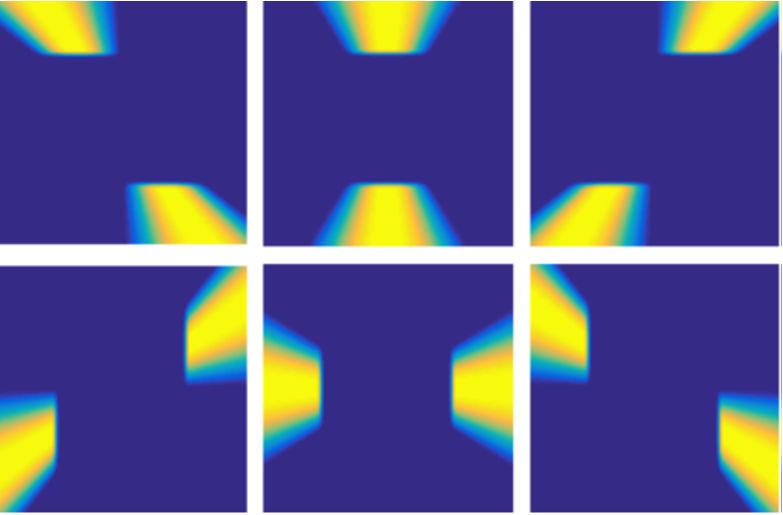
\includegraphics[width=\textwidth]{feasible_mi.pdf}
\end{minipage}
\begin{minipage}[c]{.22\textwidth}
\centering
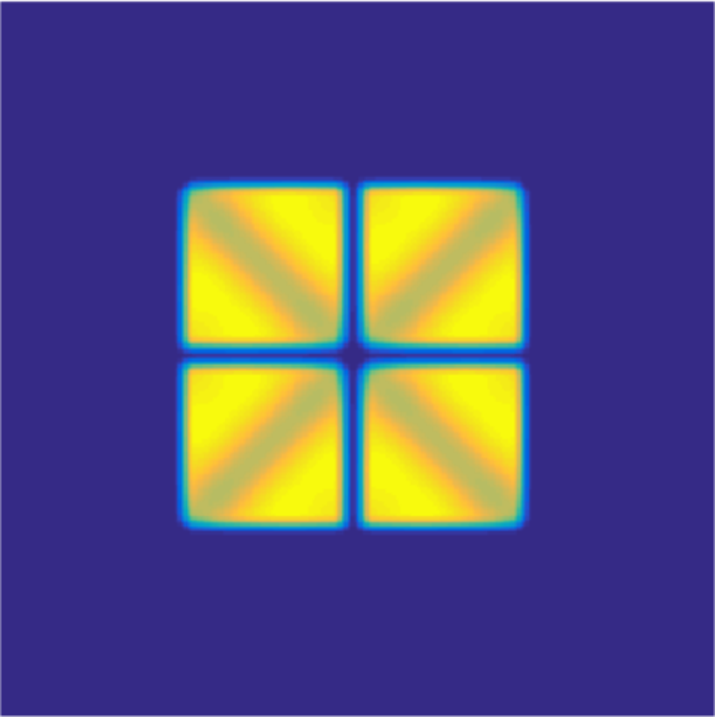
\includegraphics[width=.8\textwidth]{feasible_m0.pdf}
\end{minipage}
\begin{minipage}[c]{.28\textwidth}
\centering
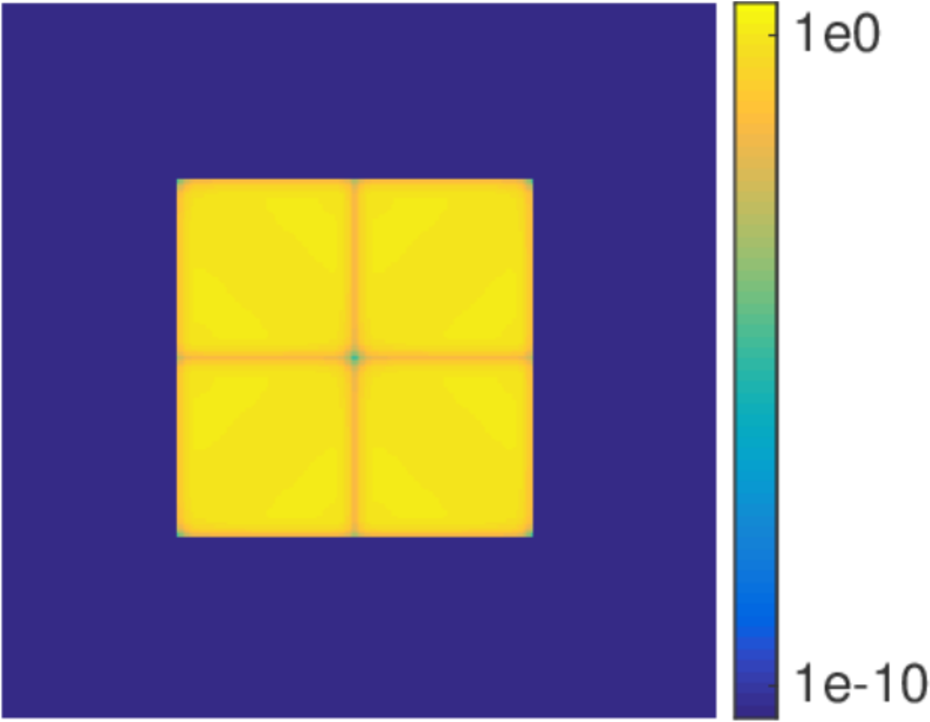
\includegraphics[width=.8\textwidth]{feasible_m0_log.pdf}
\end{minipage}
\caption{Left:  $|\m{i}|$, middle: computed $m_0^C$, right: $\log(m_0^C)$}
\label{fig: tm_i_m_0}
\end{figure}

\subsection{solving $\mc{0}$ and $m_i$}
We compute $\mc{0}$ by solving the following optimization problem similar to \eqref{eq: opt-diff} for the dyadic scheme,
\begin{align}
\min_{\xvec}\; \Vert \V{D}(\mathbf{m}_0^C\circ\xvec)\Vert^2 + \lambda\Vert \wvec\circ\mathbf{m}_0^C\circ\xvec\Vert^2,\quad 
s.t. \; A\xvec = \mathbf{1},\, \mathfrak{D}\xvec = \mathbf{0}
\label{eq: opt-2d}
\end{align}
where $\circ$ is Hadamard product and $\wvec$ is a weight vector and we consider real solution $\xvec$ here.
$A$ in the constraint is the matrix generated from the identity condition \eqref{eq: identity-cond} and $\mathfrak{D}$ is generated from the singularity condition \eqref{eq: singular-cond}. Since $A$ and $\mathfrak{D}$ are linearly independent, \eqref{eq: opt-2d} is feasible. Here, instead of optimizing the properties of $\xvec$ as in \eqref{eq: opt-diff}, we optimize those of $\widetilde{\mathbf{m}_0}^C\circ \xvec$ since $m_0^C \cdot\widetilde{m_0}^C$ will be later re-decomposed into $m_0$ and $\widetilde{m_0}$. In addition, if $m_0^C$ is symmetric with respect to the two coordinates $\omega_x$ and $\omega_y$, then we impose the same symmetry on $\widetilde{m_0}^C$ by solving \eqref{eq: opt-2d} on $[0,\pi)\times[0,\pi)$ and then extend the solution to $[-\pi,\pi)\times[-\pi,\pi)$ by symmetry.

\begin{figure}
\centering
\begin{minipage}[c]{.3\textwidth}
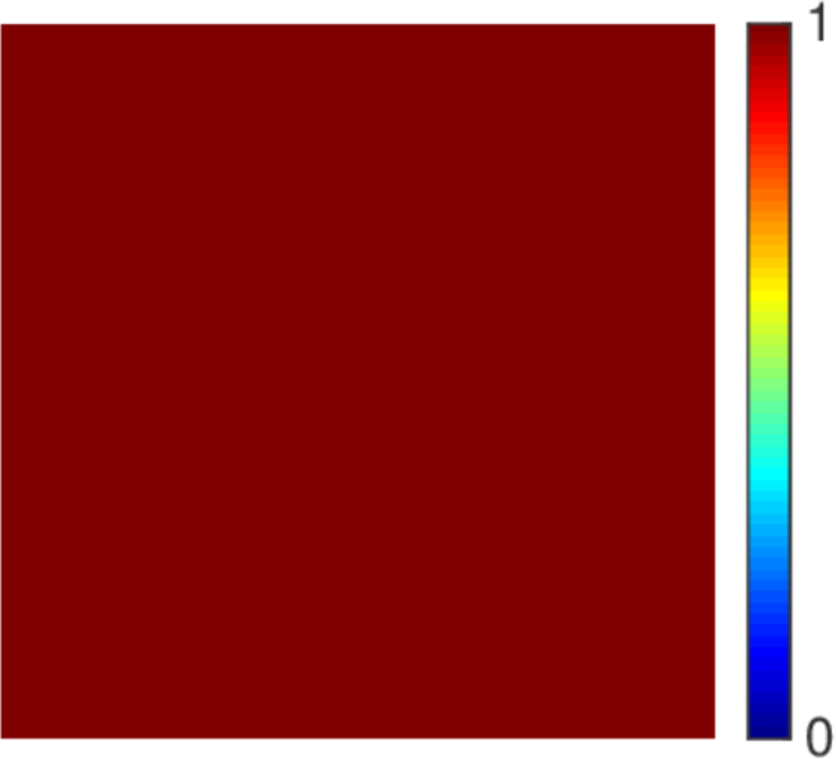
\includegraphics[width = .8\textwidth]{feasible_check.pdf}
\caption{$\vartheta$}\label{fig: feasible}
\end{minipage}
\begin{minipage}[c]{.63\textwidth}%{.28\textwidth}
\centering
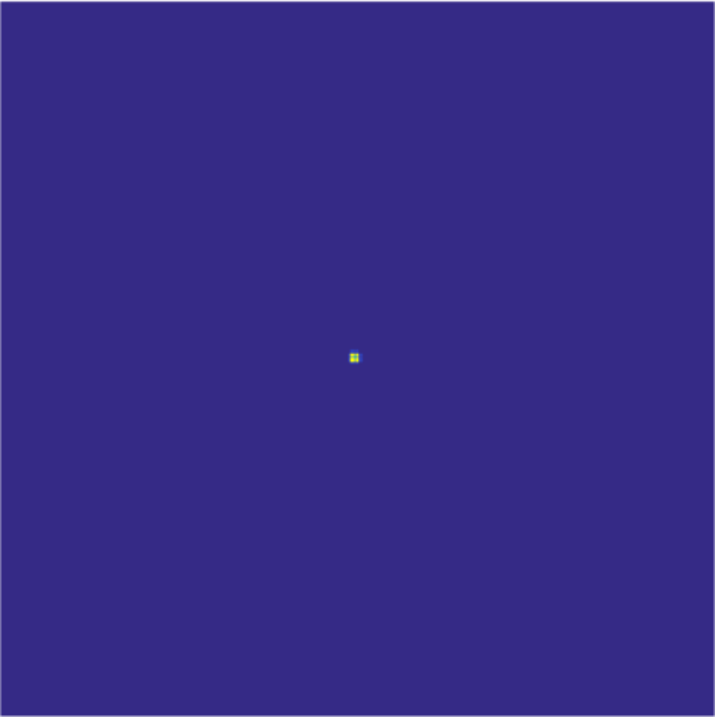
\includegraphics[width = .38\textwidth]{feasible_tm0.pdf}\hspace*{2em}
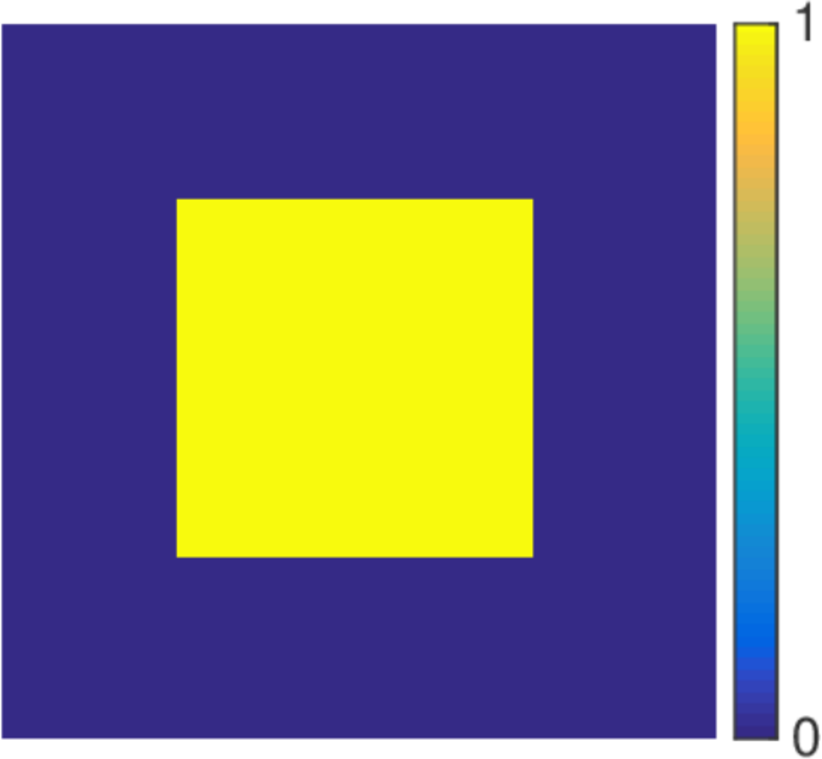
\includegraphics[width = .42\textwidth]{feasible_m0tm0.pdf}
\caption{Left: : computed $\widetilde{m_0}^C$, right: $\widetilde{m_0}^C \cdot m_0^C $}
\label{fig: tm0}
\end{minipage}
\end{figure}

Fig.\ref{fig: tm0} shows $\mc{0}$ obtained from \eqref{eq: opt-2d} and $\widetilde{m_0}^C \cdot m_0^C$ which is $\mathbf{1}_{S_1}$.

In particular, given $\widetilde{m_0}^C \cdot m_0^C = 1$, $\mathbf{b}(\V{\omega}) = \mathbf{0}, \, \forall\,\V{\omega}\in S_1$, hence $\mathbf{m}[2:7] = \mathbf{0}$. 
When $\mathbf{b}(\V{\omega})\neq \mathbf{0}$, \eqref{eq: mi} is a degenerated over-determinant linear system (we also do a sanity check here for the linearity between $\overline{\M}[:,2:7]$ and $\mathbf{b}$ by computing $\vartheta$) and 
$$\mathbf{m}[2:7](\V{\omega}) = \Big(\overline{\M}[:,2:7]\Big)^\dagger\,\mathbf{b}(\V{\omega}),$$
where $\dagger$ is the pseudo-inverse of a matrix. Fig.\ref{fig: m_i} shows the solution $m_i$ of \eqref{eq: mi} and the corresponding spatial filters $\mathcal{F}^{-1}\widetilde{m_0}$.
As shown in Fig.\ref{fig: m_i}, the energy of $m_i$ concentrates on $\{|\omega_x| = \frac{\pi}{2},\, |\omega_y| = \frac{\pi}{2}\}$ where $|\widetilde{m_i}|$ is small, and the filters decay slowly in time domain.

The bi-orthogonal bases constructed is not ideal, despite the regularization on $m_0$ in the optimization \eqref{eq: opt-2d}. Since no explicit regularization is put on $m_i$, it's difficult to control the regularity of the output $m_i$ from the input $\widetilde{m_i}$.

\begin{figure}
\centering
\begin{minipage}[c]{.5\textwidth}
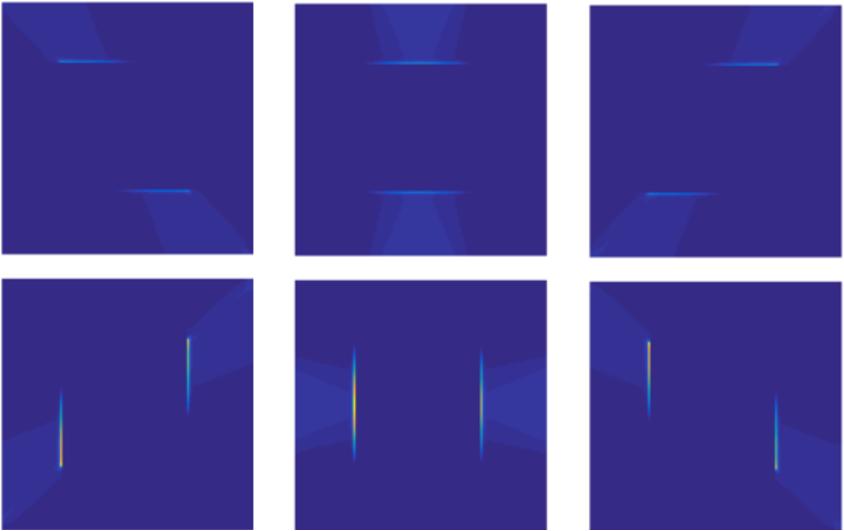
\includegraphics[width = .9\textwidth]{feasible_m.pdf}
\end{minipage}
\begin{minipage}[c]{.48\textwidth}
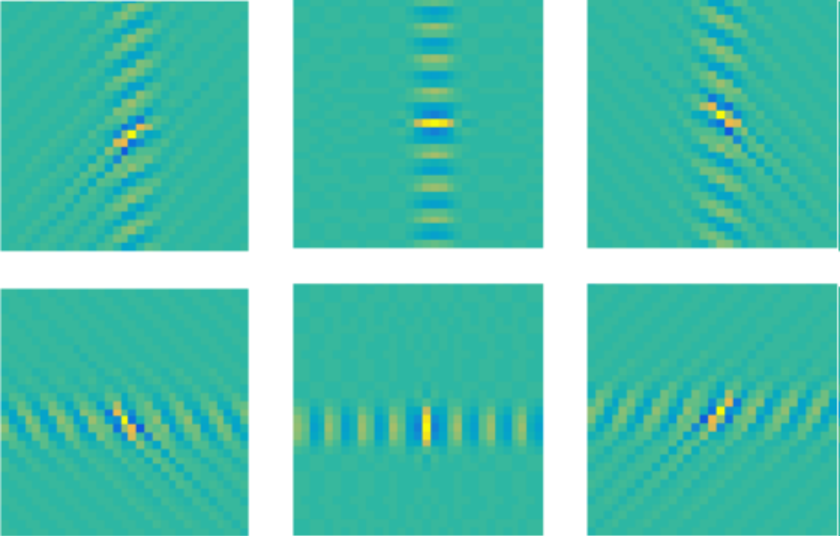
\includegraphics[width = .9\textwidth]{feasible_mi_time.pdf}
\end{minipage}
\caption{Left: $|m_i|,\, i = 1,\cdots,6$, right:$|\mathcal{F}^{-1}m_i|$}
\label{fig: m_i}
\end{figure}
\end{comment}
%\section{Bi-orthogonal Bases}\label{sec: bi-orth}
In this section, we analyze bi-orthogonal bases in the following form of MRA,
\begin{align}\label{eq: bi-orth MRA}
\{\phi_{L,\V{k}},\widetilde{\phi}_{L,\V{k}}, \psi_{l,\V{k}'}^j,\widetilde{\psi}_{l,\V{k}'}^j,\, 1\leq l\leq L,\,\V{k}\in\mathbb{Z}^2,\, \V{k}'\in\mathbf{Q}\mathbb{Z}^2,\,1\leq j\leq J \},
\end{align}
where $\phi$ and $\psi^j$ satisfy \eqref{eq: m0} and \eqref{eq: mj}, as well as $\widetilde{\phi}$ and $\widetilde{\psi^j}$, respectively,
\begin{align}\label{eq: mj_dual}
\widehat{\widetilde{\phi}}(\V{D}^T\V{\omega}) = \widetilde{m_0}(\V{\omega})\widehat{\widetilde{\phi}}(\V{\omega}),\quad \widehat{\widetilde{\psi^j}}(\V{D}^T\V{\omega}) = \widetilde{m_j}(\V{\omega})\widehat{\widetilde{\phi}}(\V{\omega}).
\end{align}
For such bi-orthogonal bases, we have the similar identity summation and shift cancellation condition to those in Theorem \ref{thm: conds}.
\begin{thm}\label{thm: bi-orth conds}
The perfect reconstruction iff the following two conditions hold
\begin{align}\label{eq: id-sum 2}
m_0(\boldsymbol{\omega})\sbarm{0} + \sum_{j = 1}^6 m_j(\boldsymbol{\omega})\sbarm{j} = 1
\end{align}
\begin{equation}\label{eq: shift-cancel 2}
\begin{cases}
\sum_{j = 0}^6m_j(\boldsymbol{\omega})\overline{\widetilde{m_j}}(\boldsymbol{\omega} + \boldsymbol{\pi}) = 0, & \boldsymbol{\pi}\in \Gamma_0\setminus\{\boldsymbol{0}\}\\[.5em]
\sum_{j=1}^6m_j(\boldsymbol{\omega})\overline{\widetilde{m_j}}(\boldsymbol{\omega}+\boldsymbol{\pi}) = 0, & \boldsymbol{\pi}\in\Gamma_1\setminus\Gamma_0
\end{cases}
\end{equation}
\end{thm}
The conditions \eqref{eq: id-sum 2} and \eqref{eq: shift-cancel 2} can be combined into a linear system as follows,
\begin{align}\label{eq: LS-new}
%\overline{\M}(\V{\omega})\mathbf{m}_0(\V{\omega})=
\begin{bmatrix}
    \,\sbarm{0} & \sbarm{1} & \hdots & \sbarm{6}\;  \\
    \;0 & \sbarmp{1}{1}  & \hdots  & \sbarmp{6}{1}\; \\
    \,\sbarmp{0}{2} & \sbarmp{1}{2} & \hdots & \sbarmp{6}{2}\;\\
    \;\vdots & \vdots & \vdots & \vdots \; \\
    \;0 & \sbarmp{1}{7} & \hdots & \sbarmp{6}{7}\;
\end{bmatrix}
\begin{bmatrix}
\;\mo{0}\; \\
\;\mo{1}\; \\
\;\mo{2}\; \\
\; \vdots\; \\
\;\mo{6}\; 
\end{bmatrix} 
=
\begin{bmatrix}
1\\
0\\
0\\
\vdots \\
0
\end{bmatrix}
\end{align}
%where $\M\in\mathbb{C}^{8\times 7}$ and $\mathbf{m}_0\in\mathbb{C}^7$.
In addition, we have the following analogue of Theorem \ref{thm: basis cond}.
\begin{thm}\label{thm: basis cond 2}
Assume that $m_0, \widetilde{m_0}$ are trigonometric polynomials with $m_0(0)=\widetilde{m_0}(0) = 1$, which generate $\phi,\widetilde{\phi}$ respectively.\\
If $\phi(\cdot - \boldsymbol{k}),\widetilde{\phi}(\cdot - \boldsymbol{k}),\,\boldsymbol{k}\in\mathbb{Z}^2$ are bi-orthogonal, then $\exists K$ containing a neighborhood of 0, s.t. $\forall\boldsymbol{\omega}\in S_0,\,\boldsymbol{\omega}+2\pi\mathbf{n}\in K$ for some $\mathbf{n}\in\mathbb{Z}^2, $ and $\inf_{k>0,\,\boldsymbol{\omega}\in K}|m_0(\mathbf{D_2}^{-k}\boldsymbol{\omega})| >0$, $\inf_{k>0,\,\boldsymbol{\omega}\in K}|\widetilde{m_0}(\mathbf{D_2}^{-k}\boldsymbol{\omega})| >0$. 
 Further, if  $\sum_{\boldsymbol{\V{\pi}}\in \Gamma_0} m_0(\boldsymbol{\omega}+\boldsymbol{\pi})\sbarmp{0}{} = 1,$ then the inverse is true.
\end{thm}
By Theorem \ref{thm: basis cond 2}, $m_0$ and $\widetilde{m_0}$ need to satisfy the following identity constraint for the MRA \eqref{eq: bi-orth MRA} to be bi-orthogonal,
\begin{align}\label{eq: identity-cond}
m_0\sbarm{0} + m_0\sbarmp{0}{2} + m_0\sbarmp{0}{4} + m_0\sbarmp{0}{6} = 1.
\end{align}
In sum, the construction of a bi-orthogonal basis \eqref{eq: bi-orth MRA} is equivalent to find feasible solutions of \eqref{eq: LS-new} with constraint \eqref{eq: identity-cond}\footnote{In fact, as long as \eqref{eq: LS-new} has a unique solution for $m_j$ given fixed $\widetilde{m_j}, \, j = 0,\cdots,6,$ \eqref{eq: identity-cond} always holds. }. To solve this, we use the same approach as in \cite{cohen1993compactly}, which constructs compactly supported symmetric bi-orthogonal filters on a hexagon lattice. We next review the main scheme in \cite{cohen1993compactly} and adapt it to our setup of directional wavelet filter.

\subsection{Summary of Cohen et al's construction}\label{subsec: cohen-summary}
We summerize the main setup and the approach in \cite{cohen1993compactly}. Consider a bi-orthogonal scheme consists of 3 high-pass filters $m_1,m_2$ and $m_3$ and a low-pass filter $m_0$ together with their bi-orthogonal duals $\widetilde{m_j}$, s.t.
$m_0$ is $\frac{2\pi}{3}$-rotation invariant and $m_1,\, m_2,\, m_3$ are $\frac{2\pi}{3}$-rotation co-variant.

This bi-orthogonal scheme satisfies the following linear system (
Lemma 2.2.2 in \cite{cohen1993compactly} )
\begin{align}\label{eq: LS}
\begin{bmatrix}
    \, \overline{\widetilde{m_0}}(\V{\omega}) &  \overline{\widetilde{m_1}}(\V{\omega}) &  \overline{\widetilde{m_2}}(\V{\omega}) &  \overline{\widetilde{m_3}}(\V{\omega})\; \\
    \;\sbarmn{0}{1} & \sbarmn{1}{1}  & \sbarmn{2}{1}  & \sbarmn{3}{1}\; \\
    \;\sbarmn{0}{2} & \sbarmn{1}{2}  & \sbarmn{2}{2}  & \sbarmn{3}{2}\; \\
    \;\sbarmn{0}{3} & \sbarmn{1}{3} & \sbarmn{2}{3} & \sbarmn{3}{3}\;
\end{bmatrix}
\begin{bmatrix}
\;\mo{0}\; \\
\;\mo{1}\; \\
\;\mo{2}\; \\
\;\mo{3}\; 
\end{bmatrix} 
=
\begin{bmatrix}
1\\
0\\
0\\
0
\end{bmatrix}
\end{align}
 where $\V{\nu}_i = \V{\pi}_i,\, i = 1,2,3.$ %$\V{\nu}_1 = (\pi,0),\V{\nu}_2 = (0,\pi),\V{\nu}_3=(\pi,\pi)$.
 Let $\widetilde{\mathbf{M}}(\V{\omega})\in\mathbb{C}^{4\times 4}$ be the matrix with entries $\sbarm{j}$ and $\mathbf{m}(\V{\omega})\in\mathbb{C}^4$ be the vector consisting of entries $m_j(\V{\omega})$ in \eqref{eq: LS}, then \eqref{eq: LS} can be written as \[\widetilde{\mathbf{M}}\, \mathbf{m} (\V{\omega})= [1,0,0,0]^\top.\]\\
Imposing that $\m{1}$, $\m{2}$ and $\m{3}$ are determined by symmetry, and invoking Lemma 2.2.2 in \cite{cohen1993compactly} leads to
\begin{align}\label{eq: m0-sol}
m_0(\V{\omega}) &= D^{-1}%\propto 
\left|
\begin{matrix}
    \; \sbarmn{1}{1}  & \sbarmn{2}{1}  & \sbarmn{3}{1}\; \\
    \; \sbarmn{1}{2}  & \sbarmn{2}{2}  & \sbarmn{3}{2}\; \\
    \; \sbarmn{1}{3} & \sbarmn{2}{3} & \sbarmn{3}{3}\;
\end{matrix}
\right| \notag\\
&= D^{-1}\widetilde{\mathbf{M}}_{0,0}(\V{\omega}),
\end{align}
where $\widetilde{\mathbf{M}}_{0,0}$ is the minor of $\widetilde{\mathbf{M}}$ and $ D \equiv \det(\widetilde{\mathbf{M}}(\V{\omega}))\in \mathbb{C}^* = \mathbb{C}\setminus\{0\}$ does not depend on $\V{\omega}$ in \cite{cohen1993compactly}, because of symmetry.
%{\it Remark.} 
%For \eqref{eq: m0-sol} to hold, $m_0(\mathbf{\omega})$ and $\det(\widetilde{\mathbf{M}}_{1,1}(\V{\omega}))$ having the same phase suffices, which is implied by the symmetry of $m_0$ and $\widetilde{m_j} $'s.\\ % Both $\mo{0}$ and $\det(\widetilde{\mathbf{M}}_{1,1}(\V{\omega}))$ are $\frac{2\pi}{3}-$rotation invariant. \\
If $\widetilde{m_0}$ is solved, then $m_1,m_2$ and $m_3$ are obtained by solving the linear system \eqref{eq: LS}.
In particular, $\m{0}$ need to satisfy 
\begin{align}\label{eq: bi-orth-eq}
m_0\sbarm{0} + m_0\sbarmn{0}{1} + m_0\sbarmn{0}{2} + m_0\sbarmn{0}{3} = 1,
\end{align}
which can be obtained by expanding $det(\widetilde{\mathbf{M}})$ with respect to the first column.
According to Lemma 3.2.1 in \cite{cohen1993compactly}, based on {\it Hilbert's Nullstellensatz}, \eqref{eq: bi-orth-eq} has a solution if and only if there does not exist $(z_1,z_2)\in (\mathbb{C}^*)^2,\, \mathbb{C}^* = \mathbb{C}\setminus\{0\}$\, s.t. $(\pm z_1,\pm z_2)$ are all 
vanishing points of the $z$-transform of $m_0$.

%\subsubsection{Solving $\m{0}$}
In general, there is no efficient algorithm to solve {\it Hilbert's Nullstellensatz}, and how \eqref{eq: bi-orth-eq} is solved exactly is not mentioned in \cite{cohen1993compactly}.
In the next section, we propose an optimization problem that solves $\widetilde{m_0}$, where \eqref{eq: m0-sol}(which is the same as \eqref{eq: identity-cond}) serves as a linear constraint and the objective function imposes regularity on $\widetilde{m_0}$.


\section{Adaptation to dilated quincunx scheme}\label{sec: solve-quincunx}

Following the same approach of Cohen et al, we first design $\m{j},\,j = 1,\cdots,6,$ then solve for $m_0,\widetilde{m_0}$ and $m_j$ in order with respect to \eqref{eq: LS-new} and \eqref{eq: identity-cond}.
%we focus on solving $m_i$'s and $\widetilde{m_0}$ in \eqref{eq: LS-new} given pre-designed $\m{i},\,i=1,\cdots,6$. %Assume $\m{i},\,i=1,\cdots,6$ satisfy weak constraints on the direction selectivity of their support.

Since \eqref{eq: LS-new} takes the same form as \eqref{eq: LS}, for simplicity, in the rest of this paper, we adapt the matrix and vector notations $\widetilde{\mathbf{M}}(\V{\omega}),\,\mathbf{m}(\V{\omega}) $ that helped to simplify \eqref{eq: LS}. Accordingly, we rewrite \eqref{eq: LS-new} as  \[\widetilde{\mathbf{M}}\, \mathbf{m} (\V{\omega})= [1,0,0,0,0,0,0]^\top,\]  where $\widetilde{\mathbf{M}}(\V{\omega})\in\mathbb{C}^{8\times 7}$ and $\mathbf{m}(\V{\omega})\in\mathbb{C}^7$. In addition, let $\V{b}_k \in\mathbb{R}^8,\, 0\leq k\leq 7$, whose only non-zero entry is $\V{b}_k[k] = 1$, where the indexing starts with zero. Note that $\M\,\mathbf{m}(\V{\omega}) = \V{b}_0\in\mathbb{R}^8$ is over-determined; it has a unique solution if and only if 

\begin{enumerate}[leftmargin=.5in]
\item[\mylabel{cond: 1}{(\ref{sec: solve-quincunx}.i)}] $\M(\V{\omega})$ is full rank,
\item[\mylabel{cond: 2}{(\ref{sec: solve-quincunx}.ii)}] $[\M(\V{\omega}), \V{b}_0]$ is singular,
\end{enumerate}
where we denote by $[\M(\V{\omega}), \V{b}_0]$ the $8\times 8$ matrix obtained by adding the 8-th column $\V{b}_0$ to the $8\times 7$ matrix $\M(\V{\omega})$.
The matrix $\M(\V{\omega})$ is structured such that each row is associated with a shift $\V{\pi}_i,\,i=0\cdots,7$ and each column is associated with a dual function $\m{j},\,j=0,\cdots,7$. We denote a sub-matrix of $\M$ containing all but the row associated with $\V{\pi}_k$(respectively, the column associated with $\m{k}$) as $\M[-k,:]$(respectively, $\M[:,-k]$).
In particular, we denote $\M[-0,-0]$ as $\Msub$.

We have the following observations for $\M(\V{\omega})$.
\begin{lemma}\label{lem: subM-singular}
If \eqref{eq: LS-new} is solvable, then $\M[-0,:](\V{\omega})$ is singular $\forall \V{\omega}$.
\end{lemma}
\noindent{\it Proof.}
If \eqref{eq: LS-new} is solvable, then condition (ii) holds, which implies that $\det([\M,\V{b}_0]) = 0$. Expanding the determinant with respect to the last column $\V{b}_0$ yields $\det(\M[-0,:]) = 0$.\qed
%If \eqref{eq: LS-new} has a solution, then $\forall \V{\omega}$,  $[1,0,\cdots,0]^\top\in \mathbb{R}^8$ is a linear combination of the columns of $\M$ hence the solution $\mathbf{m} \in Null(\M[-0,:])$ and it is non-zero. This implies that $\M[-0,:]$ is singular.\qed\\[1em]

\begin{lemma}\label{lem: M-symmetry}
$\M(\V{\omega}),\,\M(\V{\omega}+\V{\pi}_2),\,\M(\V{\omega}+\V{\pi}_4)$ and $\M(\V{\omega}+\V{\pi}_6)$ are the same up to row permutations. \eqref{eq: LS-new} holds $\forall \, \V{\omega}$ if and only if 
\begin{align*}
\M(\V{\omega}) \big[\,\mathbf{m}(\V{\omega}),\mathbf{m}(\V{\omega}+\V{\pi}_2),\mathbf{m}(\V{\omega}+\V{\pi}_4),\mathbf{m}(\V{\omega}+\V{\pi}_6)\,\big] = \big[\,\V{b}_0,\V{b}_2,\V{b}_4,\V{b}_6\,\big].
\end{align*}
\end{lemma}

Due to condition \ref{cond: 1}, $\forall\,\V{\omega}$, $\exists\, k_{\V{\omega}}$ such that $\M[-k_{\V{\omega}},:]$ is non-singular. On the other hand, Lemma \ref{lem: subM-singular} and Lemma \ref{lem: M-symmetry} together imply that $\M[-k,:],\,k=0,2,4,6$ are singular. Therefore, $k_{\V{\omega}} \in\{1,3,5,7\}$. 
As in Section \ref{subsec: cohen-summary}, we obtain the following expression of $m_0$ by applying Cramer's rule to $\M[-k_{\V{\omega}},:]$, 
%there is a unique row $\M[k_{\V{\omega}},:],\,k_\omega\in\{2,\cdots,8\}$ such that removing it from $\M$ gives a non-singular square matrix $\M[-k_{\V{\omega}},:]$. By Cramer's rule, 
\begin{align}\label{eq: m0-cramer}
m_0(\V{\omega}) = \det(\Msub[-k_{\V{\omega}},:])/\det(\M[-k_{\V{\omega}},:]).
\end{align}
Moreover, based on \eqref{eq: m0-cramer}, the identity condition \eqref{eq: identity-cond} on $m_0(\V{\omega})$ and $\m{0}$ can be derived in the same way as \eqref{eq: bi-orth-eq} by expanding $\det(\M[-k_{\V{\omega}},:])$.

In the following subsections, we first show our main result that for \eqref{eq: LS-new} to be solvable, the pre-designed $\widetilde{m_j}$'s are discontinuous, when the support of $\m{j}$ concentrates in the direction of $C_j$ and a minimum symmetry of $\m{j}$'s is required. We then discuss how to design $\widetilde{m_j}$'s with more symmetry and solve the corresponding system \eqref{eq: LS-new}.

\subsection{Discontinuity of $\m{j}$}
In this subsection, we assume that
$|\m{1}|$ and $|\m{6}|$ are symmetric with respect to the diagonal $\omega_1=\omega_2$, i.e.
$$ |\widetilde{m_1}(\V{\omega})| = |\widetilde{m_6}(\V{\omega}')|\quad \forall\, \omega_1=\omega_2', \,\omega_2=\omega_1',$$
and likewise for $\m{3}$ and $\m{4}$,
$$ |\widetilde{m_3}(\V{\omega})| = |\widetilde{m_4}(\V{\omega}')|\quad \forall\, \omega_1=-\omega_2', \,\omega_2=-\omega_1'.$$
%Same as in Section \ref{subsec: cohen-summary} , we first compute $m_0$ and assume that $\M$ is full rank, otherwise \eqref{eq: LS-new} has infinitely many solutions. Moreover, $\M[2:8,:]$ is singular. 
Let $\mrow{i}(\V{\omega}) = [\widetilde{m_1}(\V{\omega}+\V{\pi}_i)\, \cdots,\,\widetilde{m_6}(\V{\omega}+\V{\pi}_i)]\in\mathbb{C}^6,\, i = 0,\cdots,7$ be the rows of $\M[:,-0]$. 
%Proposition \ref{prop: feasibility} provides a necessary condition such that the numerical optimization solving $\widetilde{m_0}$ is feasible.
\begin{figure}
\centering
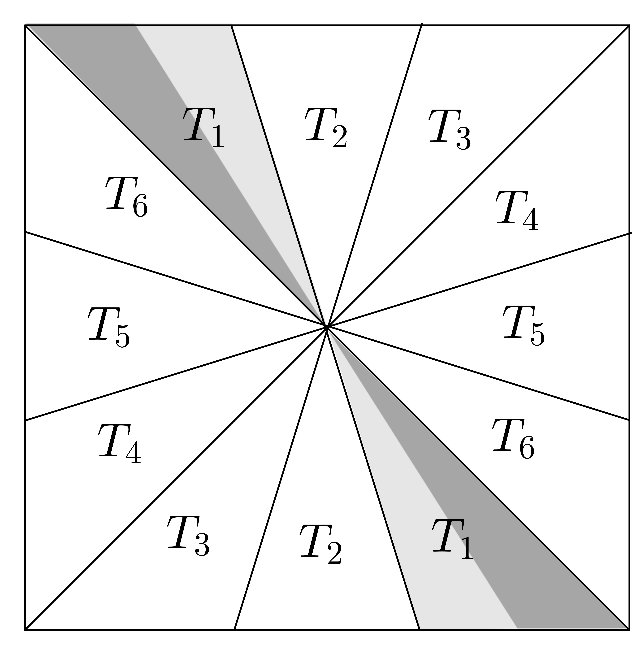
\includegraphics[width = .4\textwidth]{triangle-partition-new.png}
\caption{Partition of frequency square in six directions, where the essential support of $\m{i}$ is contained in each pair of triangles $T_i$. The pair of dark grey triangles is $T_1^-$ and the light grey pair is $T_1^+$.}
\label{fig: partition 2}
\end{figure}
%Let pairs of triangles $T_i$ in Fig.\ref{fig: partition 2} contain the essential support of $\widetilde{m_i},\,i=1,\cdots,6$.
%\eqref{eq: LS-new} takes a similar form to \eqref{eq: LS}, but with $\M\in\mathbb{C}^{8\times 7}$, which is an over-determinant linear system.
In the following, we introduce a triangular partition of frequency square and define formally the concentration of $\widetilde{m_j}$'s support.

\noindent{\bf Definition.}
The {\it essential support} $\Omega_i$ of a function $\widetilde{m_i}$ is the set $\{\V{\omega}:\,|\widetilde{m_i}(\V{\omega})|> |\widetilde{m_j}(\V{\omega})|,\,\forall j\neq i\}$. \vspace{.5em}

Let $T_i$ be pairs of triangles shown in Figure \ref{fig: partition 2}, such that $C_i\subset T_i,\, i = 1,\cdots,6.$ Consider its decomposition, $T_i = T_i^-\bigcup T_i^+$, where $T_i^-, T_i^+$ are halves of $T_i$ adjacent  to $T_{i-1}$ and $T_{i+1}$ respectively.\\[.5em]
\noindent{\bf Definition.}  $\widetilde{m_i}$ {\it concentrates} within $T_i$ if 
\begin{itemize}
\item[(i)] $\Omega_i\subset T_i$;
\item[(ii)]$\text{supp}(\widetilde{m_i})\subset T_{i-1}^+\bigcup T_i\bigcup T_{i+1}^-$ and $\int_\Omega|\widetilde{m_i}| > \int_{\Omega'}|\widetilde{m_i}|, \forall\, \Omega\subset T_i\bigcap\text{supp}(\widetilde{m_i})$, where $\Omega' \subset T_{i-1}^+\bigcup T_{i+1}^-$ is symmetric to $\Omega$ with respect to the boundary of $T_i$.
\end{itemize}

\begin{figure}
\centering
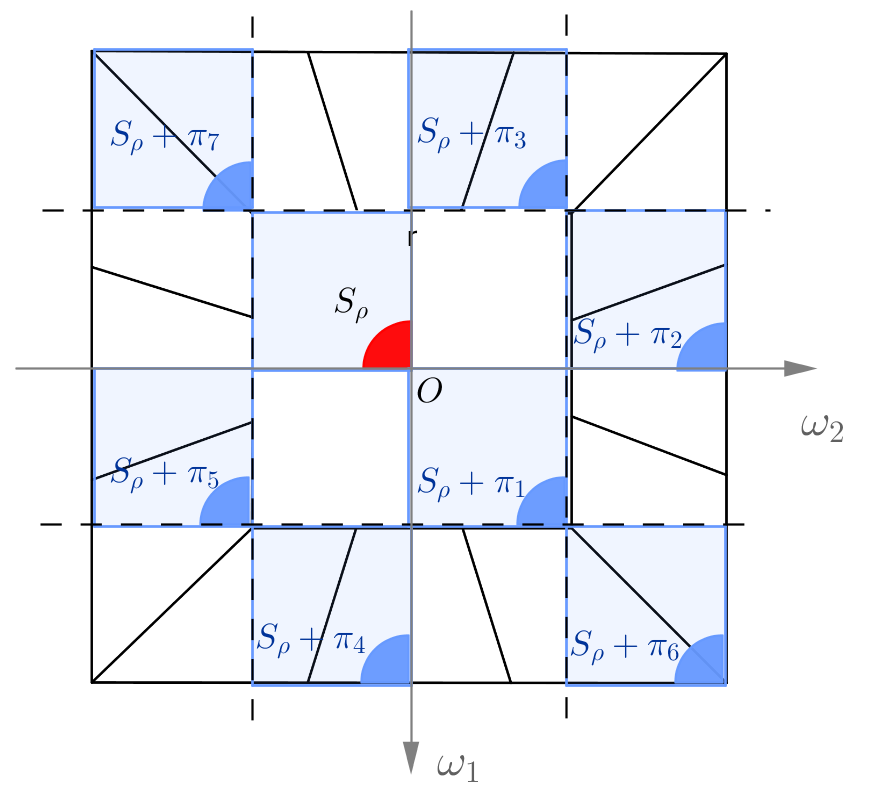
\includegraphics[width = .5\textwidth]{S_shifts2.png}
\caption{$S_{\rho}$ and its shifts}
\label{fig: S-shifts}
\end{figure}
Given $\m{i}$ that concentrates in $T_i$, we study the singularity condition on $\M[-0,:(\V{\omega})],$ specifically in the domain $S_{\rho} = \{(\omega_1,\omega_2)|\;\Vert\omega\Vert < \rho, \omega_1 <0,\,\omega_2<0\}$, see Figure \ref{fig: S-shifts}. 

\begin{lemma}\label{lem: rank1}
$\exists\, \rho>0$ s.t.  if $\M[-0,:](\V{\omega})$ is singular $\forall \V{\omega}\in S_\rho$, then $rank(\mrow{1},\mrow{7})=1$ or $rank(\mrow{3},\mrow{5}) = 1$.
\end{lemma}
Lemma \ref{lem: rank1} can be proved by analyzing the linear dependency and independency between $\mrow{i}$ on $S_\rho$, which have known locations of zero entries when $\rho$ is small due to concentration of $\widetilde{m_j}$.
For the full proof of Lemma \ref{lem: rank1}, see Appendix \ref{app: lemmas}.

Without loss of generality, in the following analysis, we assume $rank(\mrow{1},\mrow{7}) = 1$ on $S_\rho$.
Since only $\mp{1}{1}, \mp{6}{1}$ could be non-zero in $\mrow{1}$ and $\mp{1}{7}, \mp{6}{7}$ could be non-zero in $\mrow{7}$ on $S_\rho$, they are linearly related. Based on this, we can show that $\m{1},\m{6}$ are zero almost everywhere on $S_\rho + \V{\pi}_1$, which implies the discontinuity of $\m{1}$ and $\m{6}$ at $(\frac{\pi}{2},\frac{\pi}{2})$ or $(-\frac{\pi}{2},-\frac{\pi}{2})$.

\begin{proposition}\label{prop: continuity}
$\m{1},\m{6}$ are not continuous at both $(\frac{\pi}{2},\frac{\pi}{2})$ and $(-\frac{\pi}{2},-\frac{\pi}{2})$.
\end{proposition}
\noindent{\it Proof. }
If $\m{1}$ is continuous at $(\frac{\pi}{2},\frac{\pi}{2})$, then $\widetilde{m_1}(\frac{\pi}{2},\frac{\pi}{2}) = \lim_{\alpha\rightarrow 1^-}\widetilde{m_1}(\V{\omega}(\alpha)) = 0$, where $\{\V{\omega}(\alpha),\,0\leq \alpha<1\} \subset S_\rho + \V{\pi}_1$ and $\V{\omega}(1) = (\frac{\pi}{2},\frac{\pi}{2})$. By symmetry, we have $\widetilde{m_6}(\frac{\pi}{2},\frac{\pi}{2}) = 0$. Similarly, the continuity at $(-\frac{\pi}{2},-\frac{\pi}{2})$ implies $\widetilde{m_1}(-\frac{\pi}{2},-\frac{\pi}{2}) = \widetilde{m_6}(-\frac{\pi}{2},-\frac{\pi}{2}) = 0$. Therefore $\mrow{1}(0) = \mrow{7}(0) = \mathbf{0}$ which results in contradiction with Lemma \ref{lem: rank1}.\qed\\[1em]%and from \eqref{eq: m0C} $m_0^C(0)=0$ so that $m_0(0)=0$, %  On the other hand, Proposition\ref{prop: origin-det} implies that $m_0(0) = 0$ as $a = |\widetilde{m_1}(\pi_1)| = 0$, which results in contradiction.
The following theorem summarizes our main result.
\begin{theorem}\label{thm: thm}
If  $\m{i}$ concentrates in $T_i$ and $\m{1},\m{6}$ are symmetric to each other,  then  \eqref{eq: LS-new} doesn't have feasible solution given continuous $\m{1}$ and $\m{6}$.
\end{theorem}

\subsection{Design of input $\m{j}$}\label{sec: phase-design}
In this sub-section, we construct $\m{j},\, j = 1,\cdots,6,$ which concentrate in $T_i$ with high symmetry.
Specifically, following the orthonormal construction in \cite{yin2014orthshear}, we consider $\m{j}$ in the form 
\begin{align}\label{eq: m-form}
\m{j} = e^{-i\V{\eta}_j^\top\V{\omega}}|\m{j}|,\quad j = 1,\cdots,6
\end{align}
 where $|\m{j}|$'s have symmetries with respect to the two diagonals and the two axis. Figure \ref{fig: mjdual} shows such a design of $|\m{j}|$.
 
Given the symmetries of $\m{j}$, for $|m_0(\V{\omega})| > 0,\, \forall\, |\V{\omega}| < \rho$, $\V{\eta}_j$ have to satisfy certain constraints.
% We want to design the phase $\V{\eta}_k$ such that $m_0(\V{\omega}) > 0, \; \forall \omega\in S_1$. This is the same as requiring $\Msub$ to be full rank. We first show the necessary conditions on phases $\V{\eta}$ of the full rank requirement on $\Msub$.
 
\begin{lemma}\label{lem: phase-ineq}
If $\exists\,\V{\omega}\in D_1:=\{\omega_1=\omega_2,\,\omega_1\in(-\frac{\pi}{2},0)\},\,s.t. \,m_0(\V{\omega})>0,$ then $(\V{\eta}_1-\V{\eta}_6)^\top (\V{\pi}_6-\V{\pi}_7)\neq 0(\text{mod}\,2\pi)$. 
\end{lemma} 

Similarly, if $\exists\,\V{\omega}\in \{\omega_1 = \omega_2,\, \omega_1\in(0,\frac{\pi}{2})\},\, s.t.\, m_0(\V{\omega}) > 0$, then $(\V{\eta}_1-\V{\eta}_6)^\top (\V{\pi}_6-\V{\pi}_1)\neq 0(\text{mod}\,2\pi)$. These two conditions are equivalent to 
\begin{align*}
(\V{\eta}_1-\V{\eta}_6)^\top(\pi/2,\pi/2)\neq 0 (\text{mod}\,2\pi)\tag{\bf c1.1}
\end{align*}
given that $\V{\eta}_1$ and $\V{\eta}_6$ are integer phases in $\mathbb{Z}^2$.
Considering the other diagonal segment $\{\omega_2 = -\omega_1, |\omega_1| <\frac{\pi}{2}\}$, we have 
\begin{align*}
(\V{\eta}_3-\V{\eta}_4)^\top(-\pi/2,\pi/2)\neq 0 (\text{mod}\, 2\pi)\tag{\bf c1.2}
\end{align*}
%from the full rank condition.

Next, we investigate $\Msub(\V{\omega})$ at the origin.
\begin{proposition}\label{prop: origin-det}
%If $|\widetilde{m_1}(\V{\pi}_1)| = |\widetilde{m_1}(\V{\pi}_7)| = |\widetilde{m_3}(\V{\pi}_3)| = |\widetilde{m_3}(\V{\pi}_5)|$ and $|\widetilde{m_1}(\V{\pi}_6)|= | \widetilde{m_3}(\V{\pi}_6)|$, then 
If $\widetilde{m_0}(\V{0})\neq 0,$ then $\V{\pi}_1^\top(\V{\eta}_1-\V{\eta}_6)\neq \pi(\text{mod}\,2\pi)$ or $\V{\pi}_3^\top(\V{\eta}_3-\V{\eta}_4)\neq \pi(\text{mod}\,2\pi)$. 
\end{proposition}

\begin{comment}
{\it Remark.} In Lemma \ref{lem: phase-ineq}, $\Msub[:,1]$ and $\Msub[:,6]$ being independent only guarantees $\det(\Msub[-k_{\V{\omega}},:])\neq 0$. However, \eqref{eq: m0-cramer} implies that $|m_0(\V{\omega})|\propto \det(\Msub[-k_{\V{\omega}},:])$ hence it is preferred to maximize the determinant. Since
\begin{align*}
\det(\Msub[-k_{\V{\omega}}, :]) = \det\big(\big[\, \Msub[-k_{\V{\omega}},-6], \;\Msub[-k_{\V{\omega}},6] + c \cdot\Msub[-k_{\V{\omega}},1]  \,\big]\big),\quad 
\end{align*}
$\forall c\in \mathbb{C}$, the angle between $\Msub[:,1]$ and $\Msub[:,6]$ should be maximized.
Therefore, a stronger condition than ({\bf c1.1}) is to require $\Msub[:,1]$ and $\Msub[:,6]$ be orthogonal, which is equivalent to 
\begin{align*}
(\V{\eta}_1-\V{\eta}_6)^\top(\pi/2, \pi/2) = \pi \,(\text{mod}\, 2\pi).\tag{\bf c2.1}
\end{align*}
The stronger condition corresponding to ({\bf c1.2}) is 
\begin{align*}
(\V{\eta}_3-\V{\eta}_4)^\top(-\pi/2,\pi/2)=\pi(\text{mod},\,2\pi).\tag{\bf c2.2}
\end{align*} %from the stronger orthogonal condition.

%{\it Remark}
%f $|\m{1}| = |\m{2}|$ on $\{\omega_y = 3\omega_x,\,|\omega_x| > \frac{\pi}{2}\}$ and $m_0(\V{\omega}) > 0$ on $\{\omega_y = 3\omega_x\pm \pi,\,|\omega_y| <\frac{\pi}{2}\}$, then the same conditions ({\bf c1}) and ({\bf c2}) can be derived from full rank and orthogonal conditions respectively for tuples $(\,\V{\eta}_1,\,\V{\eta}_2,(-\pi/2,\pi/2)\,),\,(\,\V{\eta}_2,\V{\eta}_3,(\pi/2,\pi/2)\,),\,(\V{\eta}_4,\V{\eta}_5,\,(\pi/2,\pi/2)\,)$ and $(\,\V{\eta}_5,\V{\eta}_6,\,(-\pi/2,\pi/2)\,)$. 

% If the previous strong orthogonal condition on $\V{\eta}_1, \V{\eta}_3, \V{\eta}_4,\V{\eta}_6$ holds, then $K_1 = K_2 = 0$ and $m_0(0)=m_0^C(0)= 0$. Therefore, the strong orthogonal conditions ({\bf c2}) cannot be satisfied at the same time. 
%In particular, we consider the following constraints on phase $\V{\eta}_k\in \mathbb{Z}^2,\, k = 1,\cdots,6$:
Unfortunately, Proposition \ref{prop: origin-det} prevents ({\bf c2.1}) and ({\bf c2.2}) from holding simultaneously.
\end{comment}
We propose the following set of phases that satisfy the necessary conditions in Lemma \ref{lem: phase-ineq} and Proposition \ref{prop: origin-det},
\begin{align}\label{eq: phase-sol}
\V{\eta}_1 = (0,0),\; \V{\eta}_2 = (-1,1),\; \V{\eta}_3 = (0,2),\notag\\
\V{\eta}_4 = (1,0),\; \V{\eta}_5 = (0,-1),\; \V{\eta}_6 = (0,1).
\end{align}
\begin{comment}
where
\begin{align*}
%\label{eq: phase-constraint}
%&(\V{\eta}_1-\V{\eta}_2)^\top(-\pi/2, \pi/2) = (\V{\eta}_5-\V{\eta}_6)^\top(-\pi/2,\pi/2) = \pi\, (\text{mod}\, 2\pi)\notag\\
%&(\V{\eta}_2-\V{\eta}_3)^\top(\pi/2,\pi/2) = (\V{\eta}_4-\V{\eta}_5)^\top(\pi/2,\pi/2) = \pi\, (\text{mod}\, 2\pi)\\
%&
(\V{\eta}_3-\V{\eta}_4)^\top(-\pi/2, \pi/2) &=-\pi/2\,(\text{mod}\,2\pi)\notag\\
 (\V{\eta}_6 - \V{\eta}_1)^\top(\pi/2,\pi/2) &= \pi/2\, (\text{mod}\,2\pi)\notag
\end{align*}
%where we require strong orthogonal constraints on pair of shifts corresponding to $\widetilde{m}$ function with non-diagonal common boundary and weaker constraints on $(\V{\eta}_1,\V{\eta}_6)$ and $(\V{\eta}_3,\V{\eta}_4)$. A solution to \eqref{eq: phase-constraint} is 
\end{comment}

\subsection{Solving \eqref{eq: LS-new} and \eqref{eq: identity-cond} for $m_0,\widetilde{m_0}$ and $m_j$}\label{subsec: compute-m0}
Once $\m{j}, j= 1,\cdots, 6$ are fixed, \eqref{eq: LS-new} can be reformulated as follows,
\begin{align}\label{eq: mj-eq}
\M[:,-0](\V{\omega}) 
\begin{bmatrix}
m_1(\V{\omega})\\
m_2(\V{\omega})\\
m_3(\V{\omega})\\
m_4(\V{\omega})\\
m_5(\V{\omega})\\
m_6(\V{\omega})
\end{bmatrix}
= \V{b}_0 - m_0(\V{\omega})
\begin{bmatrix}
 \overline{\widetilde{m_0}}(\V{\omega})\\
 0\\
\sbarmp{0}{2}\\
0\\
\sbarmp{0}{4}\\
0\\
\sbarmp{0}{6}\\
0
\end{bmatrix} \doteq \V{b}_0'(\V{\omega}),
\end{align}
where $\M[:,-0]$ is determined by $\m{j},\,j = 1,\cdots,6$ 
and $m_j,\,j=1,\cdots,6$ can be uniquely solved if and only if
\hspace{-1em}
\begin{enumerate}[leftmargin=.5in]
\item[\mylabel{cond: i}{(\ref{subsec: compute-m0}.i)}] $\M[:,-0]$ is full rank,%
\item[\mylabel{cond: ii}{(\ref{subsec: compute-m0}.ii)}] $\V{b}_0'(\V{\omega})$ is in $col\big(\M[:,-0](\V{\omega})\big)$, the column space of $\M[:,-0]$.%
\end{enumerate}
%Because , \ref{cond: i} can be easily checked by computing $\det(\M[:,-0]^\top\M[:,-0])$ and see if it is non-zero. Next, we show that (ii) provides an explicit way of computing $m_0(\V{\omega})$ without knowing $\m{0}$.
Next, we show that \ref{cond: ii} breaks down to constraints on two submatrices of $\M[:,-0]$ and quadruple $\big( m_0(\V{\omega}),m_0(\V{\omega}+\V{\pi}_2), m_0(\V{\omega} +\V{\pi}_4), m_0(\V{\omega}+\V{\pi}_6) \big)$.
\begin{proposition}\label{prop: m0_formula}
Let $\M[odd,-0],\M[even,-0]\in\mathbb{C}^{4\times6}$ be the sub-matrices of $\M[:,-0]$ consisting of odd and even rows respectively. Suppose {\rm\ref{cond: i}} holds, then {\rm\ref{cond: ii}} holds if and only if $rank(\M[odd,-0]) = rank(\M[even,-0]) = 3$ and 
\begin{align}\label{eq: m0-even-null}
[m_0(\V{\omega}),m_0(\V{\omega}+\V{\pi}_2), m_0(\V{\omega} +\V{\pi}_4), m_0(\V{\omega}+\V{\pi}_6)]\, \M[even,-0](\V{\omega}) = \V{0},
\end{align}
\begin{align}\label{eq: m0-odd-null}
[m_0(\V{\omega}+\V{\pi}_1),m_0(\V{\omega}+\V{\pi}_3), m_0(\V{\omega} +\V{\pi}_5), m_0(\V{\omega}+\V{\pi}_7)] \,\M[odd,-0](\V{\omega}) = \V{0}.
\end{align}
\end{proposition}
\noindent{\it Remark.} Both conditions \eqref{eq: m0-even-null} and \eqref{eq: m0-odd-null} hold $\forall \V{\omega}\in[-\pi,\pi)\times[-\pi,\pi)$ if and only if \eqref{eq: m0-even-null} holds $\forall \V{\omega}\in [-\pi,0)\times[-\pi,0)$.

According to Proposition \ref{prop: m0_formula}, $\M[:,-0]$ (or equivalently $\widetilde{m_j}$) has to satisfy the following rank constraints for \eqref{eq: mj-eq} to be uniquely solvable, 
\begin{align}\label{eq: Mranks}
rank(\M[:,-0]) = 6,\, rank(\M[odd,-0]) = rank(\M[even,-0]) = 3.
\end{align}
Furthermore, given \eqref{eq: Mranks} holds, the quadruple  $\big( m_0(\V{\omega}),m_0(\V{\omega}+\V{\pi}_2), m_0(\V{\omega} +\V{\pi}_4), m_0(\V{\omega}+\V{\pi}_6) \big)$ can be solved by \eqref{eq: m0-even-null} upto a non-zero constant $c(\V{\omega})$. The next proposition shows that this is sufficient to obtain a feasible $m_0(\V{\omega})$.

\begin{comment}
By Lemma \ref{lem: M-symmetry}, $\M[:,-0]$ are the same at $\V{\omega},\V{\omega}+\V{\pi}_2,\V{\omega}+\V{\pi}_4$ and $\V{\omega} + \V{\pi}_6$ up to row permutations. Therefore, the columns of the matrix $\V{B}$ below should be in $col\big(\M[:,-0](\V{\omega})\big)$,
\begin{align*}
\V{B}&= \widetilde{\mathbf{m}_0}^\uparrow\otimes\mathbf{m}_0 - [\V{b}_0,\V{b}_2,\V{b}_4,\V{b}_6]\\
&\doteq
\begin{bmatrix}
 \overline{\widetilde{m_0}}(\V{\omega})\\
 0\\
\sbarmp{0}{2}\\
0\\
\sbarmp{0}{4}\\
0\\
\sbarmp{0}{6}\\
0
\end{bmatrix}
\otimes
\begin{bmatrix}
 m_0(\V{\omega})\\
 m_0(\V{\omega} + \V{\pi}_2)\\
 m_0(\V{\omega} + \V{\pi}_4)\\
 m_0(\V{\omega} + \V{\pi}_6) 
\end{bmatrix}
-
\begin{bmatrix}
1 & 0 & 0 & 0\\
0 & 0 & 0 & 0\\
0 & 1 & 0 & 0\\
0 & 0 & 0 & 0\\
0 & 0 & 1 & 0\\
0 & 0 & 0 & 0\\
0 & 0 & 0 & 1\\
0 & 0 & 0 & 0
\end{bmatrix},
\end{align*}

Let $\M[:,-0] = U\Sigma V^\top$ be the singular value decomposition of $\M[:,-0]$, such that $U(\V{\omega})\in\mathbb{C}^{8\times 6}$ consists of left singular vectors of $\M[:,-0](\V{\omega})$ and $UU^\top(\V{\omega})$ is a projection matrix of $col\big(\M[:,-0](\V{\omega})\big)$. Therefore, $\V{B}$ satisfies
\begin{align}\label{eq: cond-full}
\V{P}\V{B} = (\V{U}\V{U}^\top - \V{I}_8 )\V{B} = \V{0}\in\mathbb{C}^8,
\end{align}
 where $\V{P}$ is the projection onto $col\big(\M[:,-0](\V{\omega})\big)^\bot$, $\V{I}_8$ is the identity matrix in $\mathbb{C}^8$. Because the even rows of $\V{B}$ are all zeros, we can down-sample its rows and correspondingly the columns of $\V{P}$ and \eqref{eq: cond-full} can be reduced to 
\begin{align}
\V{P}^\downarrow\V{B}^\downarrow = \V{P}^\downarrow \big(\widetilde{\mathbf{m}_0}\otimes \mathbf{m}_0 - \V{I}_4\big) = \V{0}\in\mathbb{C}^8
\end{align}
$\V{P}^\downarrow\in\mathbb{C}^{8\times 4}$ consists of odd columns of $\V{P}$ and $\V{B}^\downarrow\in\mathbb{C}^{4\times 4}$ consists of odd rows of $\V{B}$.

Let $C_{\V{\omega}} = det(\M[-k_{\V{\omega}},:])$, then we have the following observation.
\begin{lemma}\label{lem: equal-det}
$C_{\V{\omega}} = C_{\V{\omega}+\V{\pi}_2} = C_{\V{\omega}+\V{\pi}_4} = C_{\V{\omega}+\V{\pi}_6}$
\end{lemma}
\noindent{\it Proof}
Because $\widetilde{M}(\V{\omega}+\V{\pi}_2) = P_{\V{\pi}_2}\M(\V{\omega})$ where $P_{\V{\pi}_2}$ is a row permutation matrix, it follows from the definition of $C_{\V{\omega}}$ that 
$C_{\V{\omega}} = det\big(\M[-k_{\V{\omega}},:](\V{\omega})\big) = det\big(\M[-k_{\V{\omega}+\V{\pi}_2},:](\V{\omega}+\V{\pi}_2) \big)= C_{\V{\omega}+\V{\pi}_2}$ where 
$\mathbf{1}_{k_{\V{\omega}+\V{\pi}_2}} = P_{\V{\pi}_2}\mathbf{1}_{k_{\V{\omega}}}$.
\qed\\[1em]
We assume that $m_0\in\mathbb{R}_{\geq 0}$ without phase. Let $m_0^C(\V{\omega}) = m_0(\V{\omega})|C_{\V{\omega}}|\in \mathbb{R}_{\geq 0}$ and $\mc{0} = \m{0}/|C_{\V{\omega}}|$, then Lemma \ref{lem: equal-det} implies the following.
\end{comment}


\begin{proposition}\label{prop: mc}
If $\m{j}, m_j(\V{\omega}),\,  j = 0,1,...,6$ satisfy \eqref{eq: LS-new} and \eqref{eq: identity-cond}, 
%$m_0^C(\V{\omega}),$ $\,\mc{0}, m_i(\V{\omega}),\,i = 1,...,6$ do. More generally, 
%$m_0(\V{\omega})c(\V{\omega}),\,\m{0}c(\V{\omega})^{-1}, m_i(\V{\omega}),\,i=1,...,6$ 
$m_0^c(\V{\omega})\doteq m_0(\V{\omega})c(\V{\omega}), \widetilde{m_0}^c(\V{\omega})\doteq \m{0}\overline{c}(\V{\omega})^{-1}$ and $m_j(\V{\omega}),\m{j}, \, j = 1,\cdots,6$ 
satisfy \eqref{eq: LS-new} and \eqref{eq: identity-cond} if $ c(\V{\omega}) = c(\V{\omega}+\V{\pi}_2)=c(\V{\omega}+\V{\pi}_4) = c(\V{\omega}+\V{\pi}_6) \neq 0$, i.e. $c(\V{\omega})$ is $\pi$-periodic in both $\omega_1$ and $\omega_2$.
\end{proposition}
\noindent{\it Proof. }
It suffices to show that $m_0^c(\V{\omega})\overline{\widetilde{m_0}^c}(\V{\omega} + \V{\pi}_i) = m_0(\V{\omega})\sbarmp{0}{i},\,$ when $i$ is even.\qed

%\begin{align*}
%m_0^c(\V{\omega})\overline{\widetilde{m_0}^c}(\V{\omega} + \V{\pi}_i) = m_0(\V{\omega})\sbarmp{0}{i},\quad & i \text{ is even,}\hspace{4em}\qed
%\hspace{1em}m_j^c(\V{\omega})\overline{\widetilde{m_j}^c}(\V{\omega} + \V{\pi}_i) = \big(m_j(\V{\omega})\sbarmp{j}{i}\big)c(\V{\omega})c(\V{\omega}+\V{\pi}_1)^{-1},\quad & i \text{ is odd.}\qedhere\hspace{2em}\qed
%\end{align*}

Next, we solve quadruple $(\m{0}, \mp{0}{2}, \mp{0}{4}, \mp{0}{6})$ from the identity condition \eqref{eq: identity-cond} on $[-\pi, 0)\times[-\pi, 0 )$. We reformulate it as a quadratic optimization problem that minimizes the total variation of $\sbarm{0}m_0(\V{\omega})$ as follows,
%On a $2N\times 2N$ grid $\G$ of $S_0 = [-\pi, \pi)\times[-\pi, \pi)$, s.t. $\forall \V{\omega}_j \in \G, \; \V{\omega}_j+\V{\nu}_1,\,\V{\omega}_j+\V{\nu}_2,\,\V{\omega}_j+\V{\nu}_3 \in \G$, \eqref{eq: m0-sol} is reformulated as
\begin{align}\label{eq: opt}
\min_{\xvec}\; \Vert \V{D}(\mathbf{m}_0\circ\xvec)\Vert^2,\quad 
s.t. \; \V{A}\xvec = \mathbf{1},
\end{align}
where $\V{D}$ is the gradient operator, $\circ$ is Hadamard product and $\V{A}$ is the linear operator from \eqref{eq: identity-cond}. In particular, on a $2N\times 2N$ regular grid $\G=\{\V{\omega}_i\}_{i=1}^{4N^2}$ of $[-\pi, \pi)\times[-\pi, \pi), $ \eqref{eq: identity-cond} can be rewrite as
\begin{align}
\V{A}\, \overline{\widetilde{\mathbf{m}_0}}= \mathbf{1}_{4N^2}, \label{eq: m0-A}%\\ 
%\widetilde{\mathbf{m}_0} = [\widetilde{m_0}(\V{\omega}_i)]_{\,i=1,\hdots,4N^2}&\in\mathbb{C}^{4N^2} \notag
\end{align}
where $\widetilde{\mathbf{m}_0} = [\widetilde{m_0}(\V{\omega}_i)]_{\,i=1}^{4N^2}$ and $\V{A}\in \mathbb{C}^{N^2\times 4N^2}$ is a sparse matrix with entries 
$$\V{A}_{i,j} = m_0(\V{\omega}_j)\sum_{k=0}^3\delta(\V{\omega}_j-\V{\omega}_i-\V{\pi}_{2k}), \quad \V{\omega}_j \in [-\pi,0)\times[-\pi,0).$$
%Because the set $\{\V{\omega},\, \V{\omega}+\V{\nu}_k,k=1,2,3\}$ is invariant under the shift $\V{\nu}_i,\, i = 1,2,3,$ the rows of $\V{A}$ corresponding to $\V{\omega}$ and $\V{\omega}+\V{\nu}_i$ are identical and 
%Because we only need to consider \eqref{eq: identity-cond} on $[-\pi,0)\times[-\pi,0)$, 
%rows corresponds to $\V{\omega}\in [-\pi,\pi)\times[-\pi,\pi)/\{\V{0},\,\V{\nu}_i,i=1,2,3\}$. Therefore, after removing the duplicate rows, 
%$\V{A}\in \mathbb{C}^{N^2\times 4N^2}$ and \eqref{eq: m0-A} is under-determinant. \\
%We thus use \eqref{eq: m0-A} as a linear constraint in quadratic optimization to solve $\mathbf{\widetilde{m}_0}$. Suppose that $\m{0}$ is smooth, then we build a differential operator $\V{D}$ and solve the following minimization problem:
%or
%\begin{align}
%&\min_{\mvec{0}}\; \Vert \V{D}\mvec{0}\Vert^2 + \lambda \Vert \V{A}\mvec{0} - \mathbf{1}\Vert^2 \label{eq: m0-smooth-relaxed}
%\end{align}
%The solution of \eqref{eq: m0-smooth-relaxed} is $\mvec{0} = \lambda(\lambda \V{A}^\top \V{A} + \V{D}^\top \V{D})^{-1}\V{A}^\top\mathbf{1}$.

%Or suppose $\m{0}$ decays away from the origin, then we build a diagonal weighting operator $\V{W}$, and solve the following minimization problem:
%\begin{align}\label{eq: opt-weight}
%&\min_{\mvec{0}}\; \Vert \V{W}\mvec{0}\Vert^2,\quad s.t. \; \V{A}\mvec{0} = \mathbf{1}
%\end{align}
Supplementary numerical results on solving $\m{0}$ by optimization are provided in Appendix \ref{app: supp-numerical}, where we test this optimization method on known bi-orthogonal filters $m_0$ and $\widetilde{m_0}$ and compare the solution from the optimization with the ground truth.

Finally, we plug $m_0(\V{\omega})$ and $\m{0}$ into $\V{b}_0'(\V{\omega})$ on the right of \eqref{eq: mj-eq} and solve the linear system, which has a guaranteed unique solution.

%According to Proposition \ref{prop: mc}, we can first solve $\mc{0}$ and $m_0^C(\V{\omega})$ and then construct $c(\V{\omega})$ for optimal $\m{0}$ and $m_0(\V{\omega})$. 
%In particular, $m_0^C$ can be computed without knowing $k_{\V{\omega}}$,
%\begin{align}\label{eq: m0C}
%m_0^C(\V{\omega}) = m_0(\V{\omega})|C_{\V{\omega}}| = |det(\M_{1,1}[-k_{\V{\omega}},:])| = \prod_{i=1}^6\sigma_i(\M_{1,1}[-k_{\V{\omega}},:]) = \prod_{i=1}^6\sigma_i(\M_{1,1}).
%\end{align}
%In practice, we first perform QR decomposition on $\Msub:=\M_{1,1}$ and then take the absolute value of the product of the diagonal entries of the upper triangular matrix, $diag(R)$. 
To sum up, we propose the following algorithm for bi-orthogonal directional filter construction with dilated quincunx downsampling scheme:\\
\rule{\textwidth}{.5pt}
\begin{description}% prevent items from splitting
\item[construction of $m$-, $\widetilde{m}$-functions in bi-orthogonal basis]\
\begin{itemize}
\item[Input:] $\m{j},\,j=1,...,6$
\item[step 1.] construct $\M[:,-0](\V{\omega})$ on sub-grid $[-\pi,0)\times[-\pi,0)$ and check rank constraints \eqref{eq: Mranks}.%compute $m_0^C(\V{\omega}) = \left|det(\M_{1,1}[-k_{\V{\omega}},:])\right|$
\item[step 2.] solve quadruple $\big( m_0(\V{\omega}),m_0(\V{\omega}+\V{\pi}_2), m_0(\V{\omega} +\V{\pi}_4), m_0(\V{\omega}+\V{\pi}_6) \big)$ using \eqref{eq: m0-even-null} on $[-\pi,0)\times[-\pi,0)$,%compute $\mc{0}$, such that \eqref{eq: LS-new} is solvable and \eqref{eq: identity-cond} holds
\item[step 3.] solve the optimization \eqref{eq: opt} for $\m{0}$ on grid $[-\pi,\pi)\times[-\pi,\pi)$.
%solve $m_i(\V{\omega}),\, i=1,...,6$ according to \eqref{eq: LS-new}
\item[step 4.] solve the reduced linear system \eqref{eq: mj-eq} for $m_j(\V{\omega}),\, j = 1,\cdots,6$.%design $c(\V{\omega})$ and let $m_0(\V{\omega}) = m_0^C(\V{\omega})c(\V{\omega}),\,\m{0} = \mc{0}\overline{c}(\V{\omega})^{-1}$
\end{itemize}
\end{description}
\rule{\textwidth}{.5pt}\\[.5em]

Proposition \ref{prop: mc} suggests that we can design $c(\V{\omega})$ such that $(m_0^c,\widetilde{m_0}^c)$ have desired properties, e.g. continuity, smoothness or fast decay rate. In practice, we compute $m_0(\V{\omega})\sbarm{0}$ from $m_0(\V{\omega})$ and $\m{0}$ obtained in step 2 and 3, then re-decompose the product into $m_0^c(\V{\omega})$ and $\overline{\widetilde{m_0}^c}(\V{\omega})$.

We may also manipulate pairs of $(m_j,\widetilde{m_j})$ in a similar way due to the following generalization of Proposition \ref{prop: mc}.
\begin{proposition}\label{prop: mjc}
If $\m{j}, m_j(\V{\omega}),\,  j = 0,1,...,6$ satisfy \eqref{eq: LS-new} and \eqref{eq: identity-cond}, 
$m_j^c(\V{\omega})\doteq m_j(\V{\omega})c_j(\V{\omega}), \widetilde{m_j}^c_j(\V{\omega})\doteq \m{j}\overline{c}(\V{\omega})^{-1} \, j = 0,\cdots,6$ 
satisfy \eqref{eq: LS-new} and \eqref{eq: identity-cond} if $ c_0(\V{\omega}) = c_0(\V{\omega}+\V{\pi}_{2k})\,,\forall k = 0,\cdots,3$ and $c_j(\V{\omega}) = c_j(\V{\omega} + \V{\pi}_k),\, \forall \;k = 0,\cdots,7,\, j = 1,\cdots,6$.
\end{proposition}

\begin{comment}
\subsection{solving $m_i$}
In the final step, we substitute $\mc{0}$ and $m_0^C(\V{\omega})$ into \eqref{eq: LS-new} and rewrite it into the following linear system,
\begin{align}\label{eq: mi}
\overline{\M}[:,2:7]\,\mathbf{m}[2:7](\V{\omega}) = 
\begin{bmatrix}
1-m_0^C\overline{\widetilde{m_0}^C}(\V{\omega})\\
0\\
-m_0^C\overline{\widetilde{m_0}^C}(\V{\omega}+\V{\pi}_2)\\
\vdots \\
0
\end{bmatrix}
=:\mathbf{b}(\V{\omega}).
\end{align}
The solution of \eqref{eq: mi} depends only on $m_0^C\overline{\widetilde{m_0}^C}$, or equivalently $m_0\overline{\widetilde{m_0}}$. 
\end{comment}

\section{Numerical Experiments}

In this section, we show an example of the numerical construction of biorthogonal directional wavelets on a quincunx lattice using our proposed algorithm in Matlab.

We design $\widetilde{m_j}$ in the form of \eqref{eq: m-form}, using phases in \eqref{eq: phase-sol} and amplitudes $|\widetilde{m_j}|$ shown in Figure \ref{fig: mjdual}. For the construction of $|\widetilde{m_j}|$, we start with $|\widetilde{m_2}|$, then compute $|\widetilde{m_1}|$ and $|\widetilde{m_3}|$ by shearing $|\widetilde{m_2}|$ counter-clockwise and clockwise respectively. $|\widetilde{m_4}|, |\widetilde{m_5}|$ and $|\widetilde{m_6}|$ are obtained by symmetry along the diagonal. This is the same approach used in the shearlet construction \cite{kutyniok2012digital}. Furthermore, $\m{j} = 0,\,\forall \V{\omega}\in C_0 = [-\frac{\pi}{2},\frac{\pi}{2})\times [-\frac{\pi}{2},\frac{\pi}{2}).$ In particular, by Proposition \ref{prop: continuity}, we enforce $|\widetilde{m_1}(\frac{\pi}{2},\frac{\pi}{2})|\neq 0$ and $\widetilde{m_6}(\frac{\pi}{2},\frac{\pi}{2})|\neq 0$.

Using these $\m{j},\,j = 1,\cdots,6$ as input, the main algorithm in Section \ref{subsec: compute-m0} yields $m_0,\widetilde{m_0}$ and $m_j, \, j = 1,\cdots, 6$. As the first step, we numerically check that this particular design of $\widetilde{m_j}$ satisfies the rank constraints \eqref{eq: Mranks}. As shown in Figure \ref{fig: m_0} $m_0(\V{\omega})$ obtained in step 2 is supported on the central square $C_0$, where $|m_0(\V{\omega})| = 1$. Moreover, Figure \ref{fig: m_0_m0dual} shows that $\m{0} = \overline{m_0^{-1}}(\V{\omega}) = m_0(\V{\omega})$ on $C_0$, i.e. $\m{0}$ solved in step 3 is numerically the same as $m_0(\V{\omega})$.
Figure \ref{fig: m_j} and Figure \ref{fig: m_j_mjdual} show $|\m{j}|$ and $|m_j\m{j}|$ for $\m{j}$ obtained by solving \eqref{eq: mj-eq}. We also numerically check that $m_j(\V{\omega})$ and $\m{j}$ have the same phase, i.e. $m_j\m{j}\in \mathbb{R}$.

So far, we construct a set of $(m_j,\widetilde{m_j})_{j = 0,\cdots,6}$ that satisfies \eqref{eq: LS-new} and \eqref{eq: identity-cond}, thus it can be used to construct biorthogonal wavelets based on \eqref{eq: mj} and \eqref{eq: mj_dual}. However, $m_0$ and $\widetilde{m_0}$ here are not continuous. To improve the regularity of the corresponding wavelets, by Proposition \ref{prop: mc} and the observation $m_0\sbarm{0} = \V{1}_{C_0}$, we replace $(m_0,\widetilde{m_0})$ by $(m_0', \widetilde{m_0}')$, where $\widetilde{m_0}'$ is a smooth real function supported on $C_0$ and $m_0'(\V{\omega}) = \V{1}_{C_0}(\overline{\widetilde{m_0}'})^{-1}(\V{\omega})$. Figure \ref{fig: smooth_m0dual} shows such a pair of $(m_0',\widetilde{m_0}')$. Finally, using pre-designed $\m{j}$ and post-designed $\widetilde{m_0}'$, we construct the dual wavelets  $\widetilde{\psi^j}$ in \eqref{eq: bi-orth MRA} using \eqref{eq: mj_dual}. As shown in Figure \ref{fig: wavelets}, the dual wavelets are spatially localized and have good direction selection. The wavelets and scaling functions in \eqref{eq: bi-orth MRA} can be constructed using \eqref{eq: mj_dual} similarly.

\begin{figure}
\centering
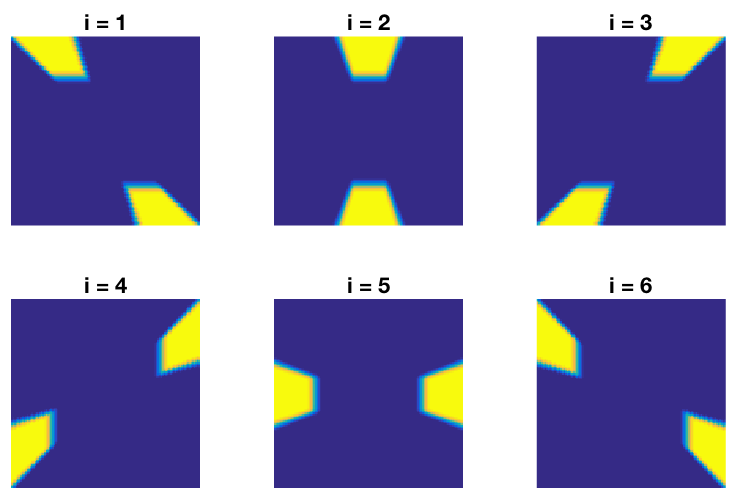
\includegraphics[width=.8\textwidth]{initialize_mdual.png}
\caption{ Input $|\m{j}|$ constructed in the same way as shearlets.}
\label{fig: mjdual}
\end{figure}

\begin{figure}
\centering
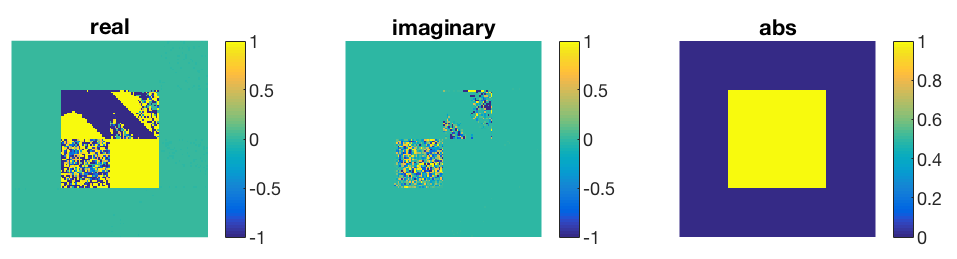
\includegraphics[width=\textwidth]{m0.png}
\caption{ $m_0(\V{\omega})$ constructed from $\widetilde{m_j}$. Left to right: $Re(m_0(\V{\omega})),\, Im(m_0(\V{\omega}))$ and $|m_0(\V{\omega})|$.}
\label{fig: m_0}
\end{figure}

\begin{figure}
\centering
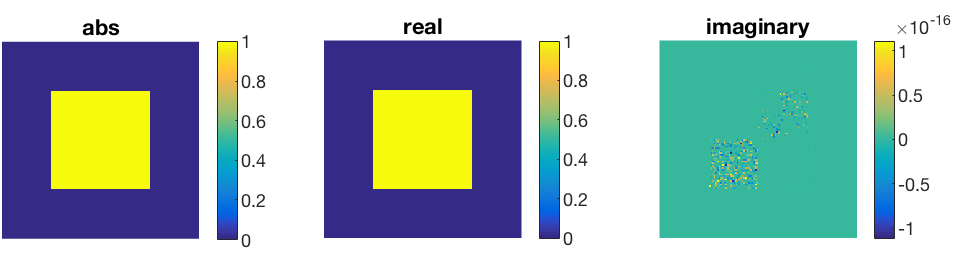
\includegraphics[width=\textwidth]{m0_m0dual_new.png}
\caption{$|\m{0}|$ and $m_0\sbarm{0}$, where $\m{0}$ is solved by optimization \eqref{eq: opt}, given $\widetilde{m_j}$ in Figure \ref{fig: mjdual} and $m_0$ in Figure \ref{fig: m_0}. Left to right: $|\m{0}|$, $Re(m_0\sbarm{0})$ and $Im(m_0\sbarm{0})$. }
\label{fig: m_0_m0dual}
\end{figure}

\begin{figure}
\centering
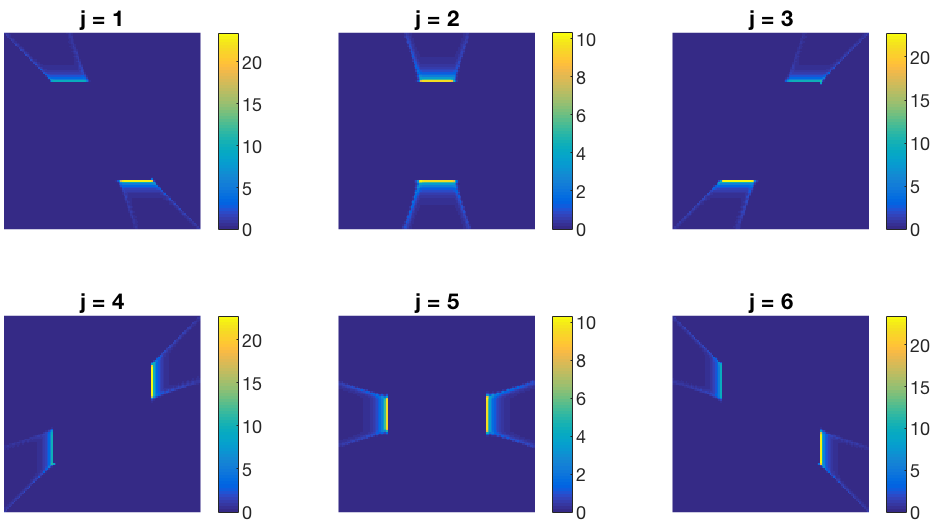
\includegraphics[width=\textwidth]{m.png}
\caption{ $|m_j(\V{\omega})|$, where $m_j(\V{\omega})$ is solved from \eqref{eq: mj-eq} given $\widetilde{m_j}$ in Figure \ref{fig: mjdual}, $m_0$ in Figure \ref{fig: m_0} and $\widetilde{m_0}$ in Figure \ref{fig: m_0_m0dual}. }
\label{fig: m_j}
\end{figure}

\begin{figure}
\centering
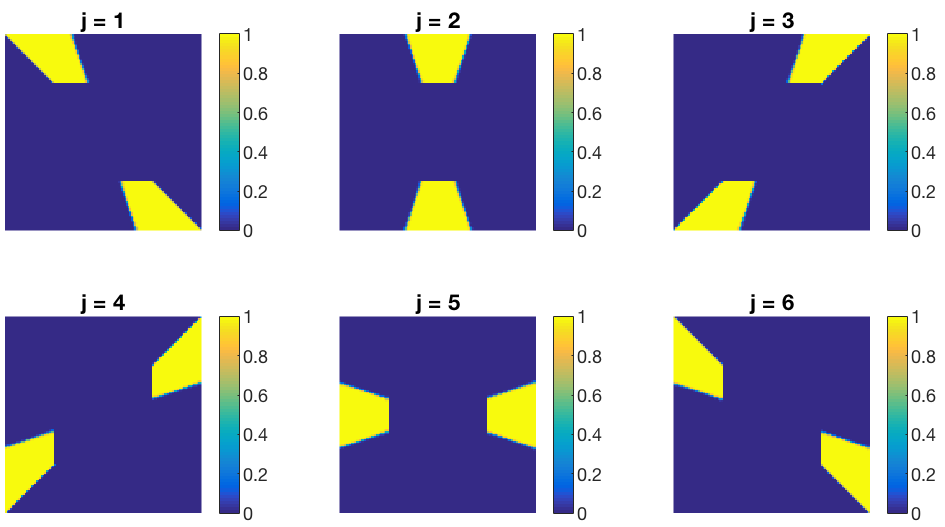
\includegraphics[width=\textwidth]{m_mdual.png}
\caption{ $|m_j(\V{\omega})\m{j}|$ }
\label{fig: m_j_mjdual}
\end{figure}

\begin{figure}
\centering
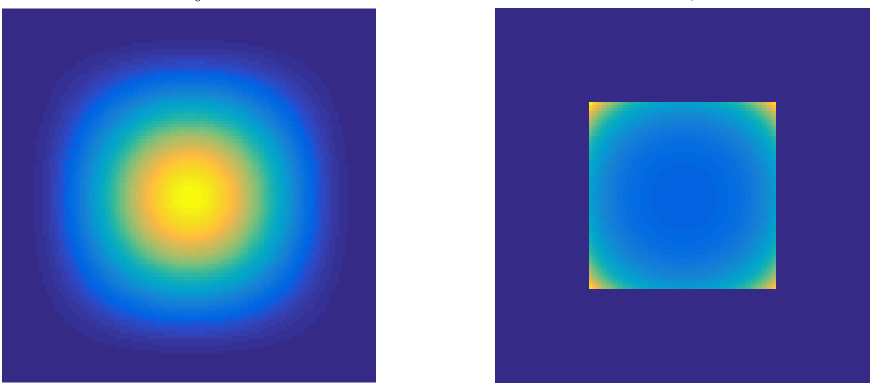
\includegraphics[width=.66\textwidth]{smooth_m0dual.png}
\caption{ Left: $\widetilde{m_0}'$, designed smooth function mainly supported on the central square $C_0$, right: $m_0'$, $s.t. m_0'\overline{\widetilde{m_0}'}(\V{\omega})  =  m_0\overline{\widetilde{m_0}}(\V{\omega})= \V{1}_{C_0}(\V{\omega})$. } 
\label{fig: smooth_m0dual}
\end{figure}

\begin{figure}
\centering
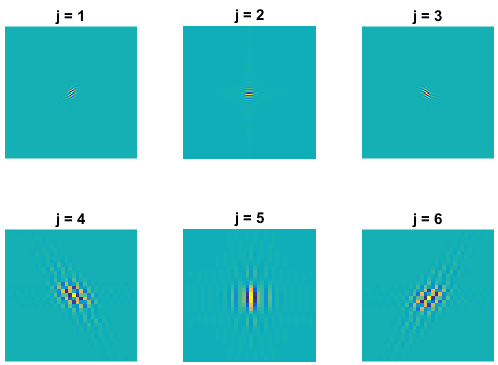
\includegraphics[width=.8\textwidth]{quincunx_wavelets.png}
\caption{ Real part of $\psi^j$ constructed from $\widetilde{m_0}'$ in Figure \ref{fig: smooth_m0dual} and $\widetilde{m_j},\, j=1,\cdots, 6$ in Figure \ref{fig: mjdual} using \eqref{eq: mj_dual}. Top: $\widetilde{\psi^j}$ without scaling, bottom: $\widetilde{\psi^j}$ with eight time zoom-in } 
\label{fig: wavelets}
\end{figure}


\begin{comment}
\subsection{solving $m_0^C$}
A set of $\m{i}$ that satisfy the conditions of Theorem \ref{thm: thm} with phase terms in \eqref{eq: phase-sol} is used as the input of \eqref{eq: LS-new}.
The left figure in Fig.\ref{fig: tm_i_m_0} shows the absolute value of $\m{i}$. In particular, $\m{i} =0,\,\forall \omega\in S_1$. 
We follow the construction process in Section \ref{subsec: compute-m0} and obtain $m_0^C$ shown in the right of Fig.\ref{fig: tm_i_m_0}, in both normal scale and log scale.  
We perform a numerical sanity check on the necessary condition in Proposition \ref{prop: feasibility}, that is $\forall\,\V{\omega}, \,s.t. [m_0(\V{\omega}), m_0(\V{\omega}+\V{\pi}_2),m_0(\V{\omega}+\V{\pi}_4),m_0(\V{\omega}+\V{\pi}_6)]$ is not a linear combination of the rows of $\mathfrak{D}(\V{\omega})$ in \eqref{eq: singular-cond}. Equivalently, we compute the following quantity $$\vartheta = 1 - \Vert V^\top\mathfrak{m}_0 \Vert/\Vert \mathfrak{m}_0\Vert ,$$ where $\mathfrak{m}_0(\V{\omega})=[m_0(\V{\omega}), m_0(\V{\omega}+\V{\pi}_2),m_0(\V{\omega}+\V{\pi}_4),m_0(\V{\omega}+\V{\pi}_6)]^\top$ and $V$ are the left singular vectors of $\mathfrak{D}(\omega)$ whose corresponding singular values are non-zero. If $\mathfrak{m}_0\in span(V)$, then $\vartheta = 0$. If $\mathfrak{m}_0\bot span(V)$, then $\vartheta = 1$.
Fig.\ref{fig: feasible} shows the feasibility check $\vartheta$ of input $\m{i}$, and $\mathfrak{m}_0$ is orthogonal to $span(V)$ everywhere.

\begin{figure}
\centering
\begin{minipage}[c]{.48\textwidth}
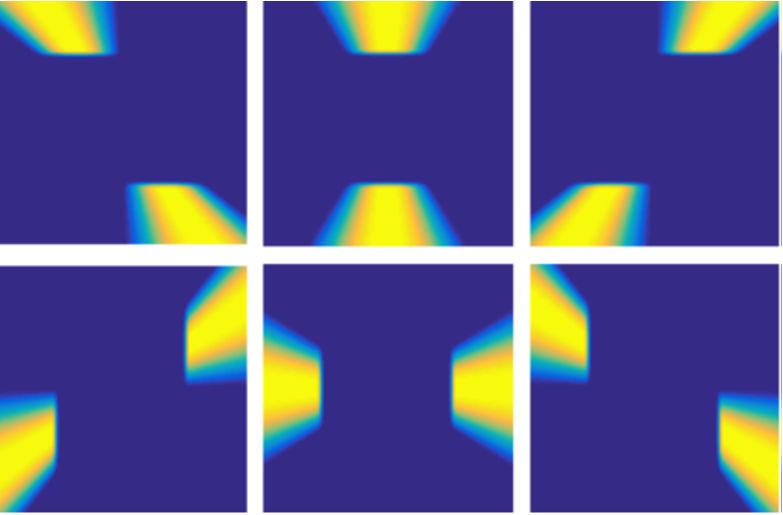
\includegraphics[width=\textwidth]{feasible_mi.pdf}
\end{minipage}
\begin{minipage}[c]{.22\textwidth}
\centering
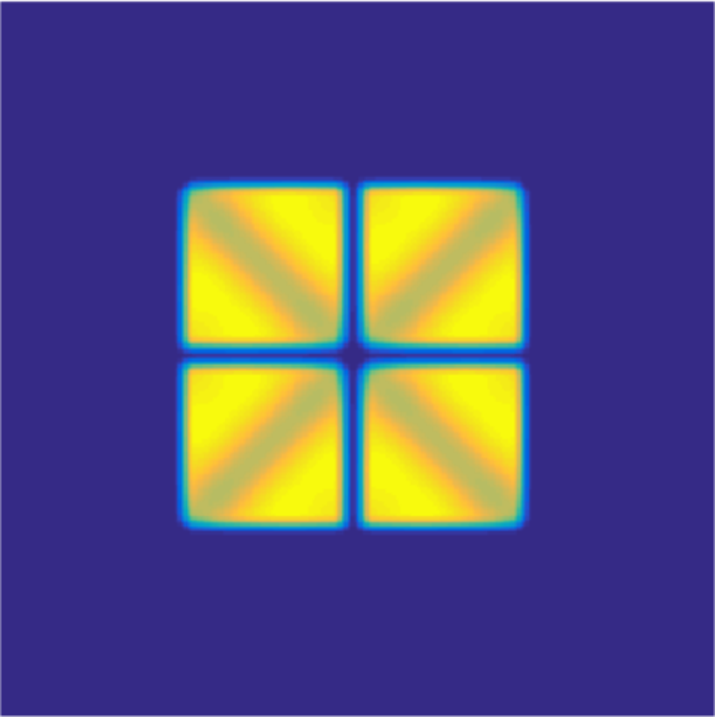
\includegraphics[width=.8\textwidth]{feasible_m0.pdf}
\end{minipage}
\begin{minipage}[c]{.28\textwidth}
\centering
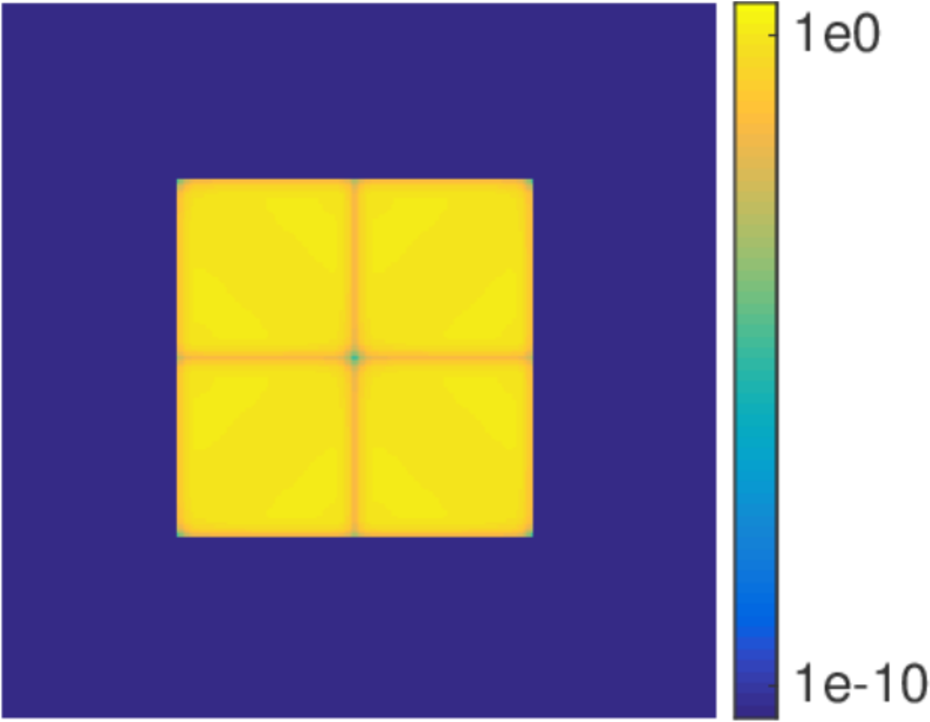
\includegraphics[width=.8\textwidth]{feasible_m0_log.pdf}
\end{minipage}
\caption{Left:  $|\m{i}|$, middle: computed $m_0^C$, right: $\log(m_0^C)$}
\label{fig: tm_i_m_0}
\end{figure}

\subsection{solving $\mc{0}$ and $m_i$}
We compute $\mc{0}$ by solving the following optimization problem similar to \eqref{eq: opt-diff} for the dyadic scheme,
\begin{align}
\min_{\xvec}\; \Vert \V{D}(\mathbf{m}_0^C\circ\xvec)\Vert^2 + \lambda\Vert \wvec\circ\mathbf{m}_0^C\circ\xvec\Vert^2,\quad 
s.t. \; A\xvec = \mathbf{1},\, \mathfrak{D}\xvec = \mathbf{0}
\label{eq: opt-2d}
\end{align}
where $\circ$ is Hadamard product and $\wvec$ is a weight vector and we consider real solution $\xvec$ here.
$A$ in the constraint is the matrix generated from the identity condition \eqref{eq: identity-cond} and $\mathfrak{D}$ is generated from the singularity condition \eqref{eq: singular-cond}. Since $A$ and $\mathfrak{D}$ are linearly independent, \eqref{eq: opt-2d} is feasible. Here, instead of optimizing the properties of $\xvec$ as in \eqref{eq: opt-diff}, we optimize those of $\widetilde{\mathbf{m}_0}^C\circ \xvec$ since $m_0^C \cdot\widetilde{m_0}^C$ will be later re-decomposed into $m_0$ and $\widetilde{m_0}$. In addition, if $m_0^C$ is symmetric with respect to the two coordinates $\omega_x$ and $\omega_y$, then we impose the same symmetry on $\widetilde{m_0}^C$ by solving \eqref{eq: opt-2d} on $[0,\pi)\times[0,\pi)$ and then extend the solution to $[-\pi,\pi)\times[-\pi,\pi)$ by symmetry.

\begin{figure}
\centering
\begin{minipage}[c]{.3\textwidth}
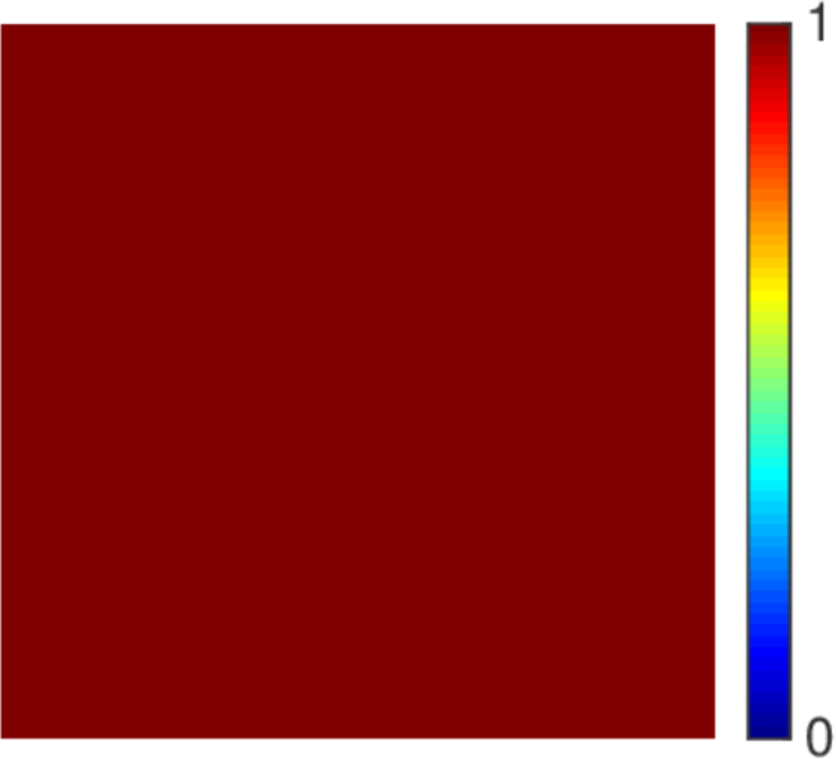
\includegraphics[width = .8\textwidth]{feasible_check.pdf}
\caption{$\vartheta$}\label{fig: feasible}
\end{minipage}
\begin{minipage}[c]{.63\textwidth}%{.28\textwidth}
\centering
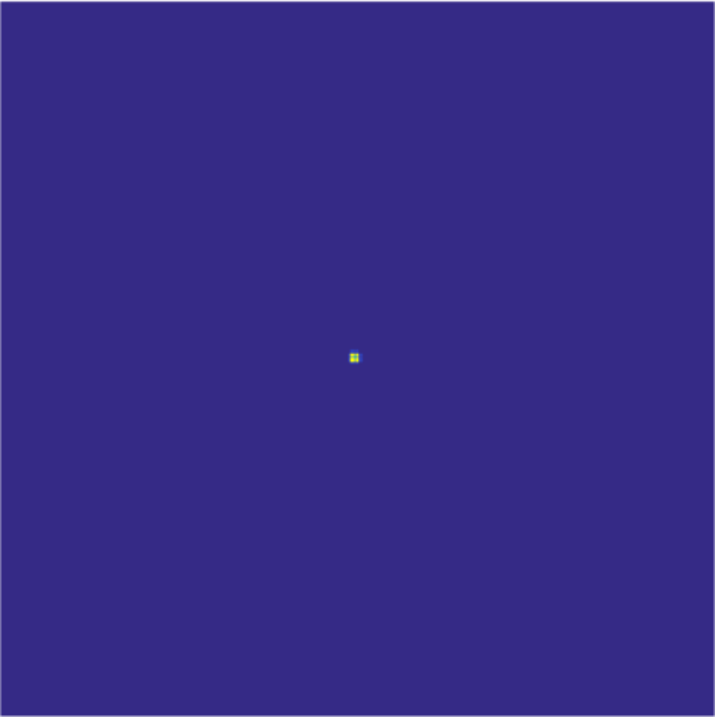
\includegraphics[width = .38\textwidth]{feasible_tm0.pdf}\hspace*{2em}
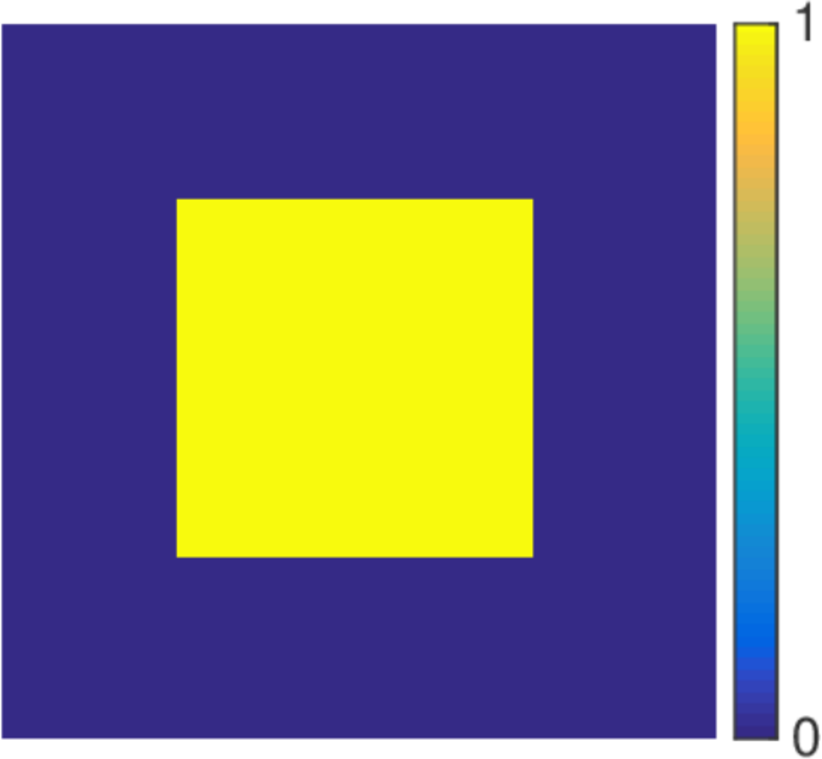
\includegraphics[width = .42\textwidth]{feasible_m0tm0.pdf}
\caption{Left: : computed $\widetilde{m_0}^C$, right: $\widetilde{m_0}^C \cdot m_0^C $}
\label{fig: tm0}
\end{minipage}
\end{figure}

Fig.\ref{fig: tm0} shows $\mc{0}$ obtained from \eqref{eq: opt-2d} and $\widetilde{m_0}^C \cdot m_0^C$ which is $\mathbf{1}_{S_1}$.

In particular, given $\widetilde{m_0}^C \cdot m_0^C = 1$, $\mathbf{b}(\V{\omega}) = \mathbf{0}, \, \forall\,\V{\omega}\in S_1$, hence $\mathbf{m}[2:7] = \mathbf{0}$. 
When $\mathbf{b}(\V{\omega})\neq \mathbf{0}$, \eqref{eq: mi} is a degenerated over-determinant linear system (we also do a sanity check here for the linearity between $\overline{\M}[:,2:7]$ and $\mathbf{b}$ by computing $\vartheta$) and 
$$\mathbf{m}[2:7](\V{\omega}) = \Big(\overline{\M}[:,2:7]\Big)^\dagger\,\mathbf{b}(\V{\omega}),$$
where $\dagger$ is the pseudo-inverse of a matrix. Fig.\ref{fig: m_i} shows the solution $m_i$ of \eqref{eq: mi} and the corresponding spatial filters $\mathcal{F}^{-1}\widetilde{m_0}$.
As shown in Fig.\ref{fig: m_i}, the energy of $m_i$ concentrates on $\{|\omega_x| = \frac{\pi}{2},\, |\omega_y| = \frac{\pi}{2}\}$ where $|\widetilde{m_i}|$ is small, and the filters decay slowly in time domain.

The bi-orthogonal bases constructed is not ideal, despite the regularization on $m_0$ in the optimization \eqref{eq: opt-2d}. Since no explicit regularization is put on $m_i$, it's difficult to control the regularity of the output $m_i$ from the input $\widetilde{m_i}$.

\begin{figure}
\centering
\begin{minipage}[c]{.5\textwidth}
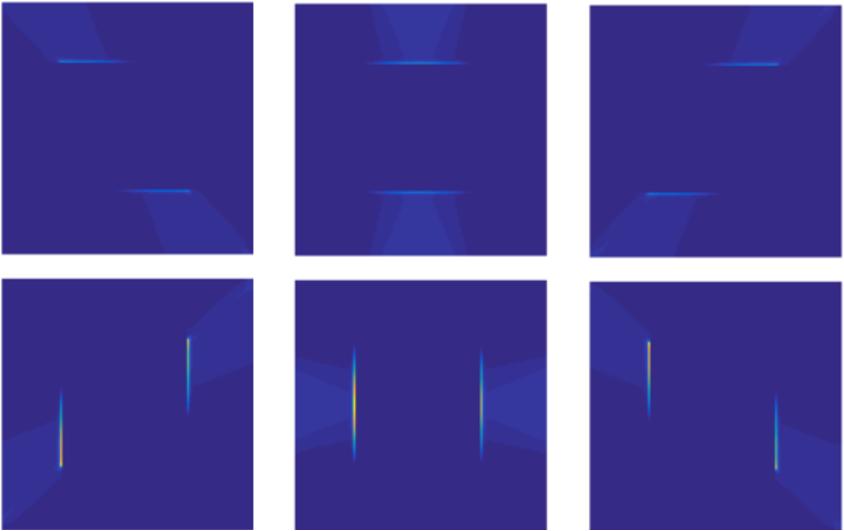
\includegraphics[width = .9\textwidth]{feasible_m.pdf}
\end{minipage}
\begin{minipage}[c]{.48\textwidth}
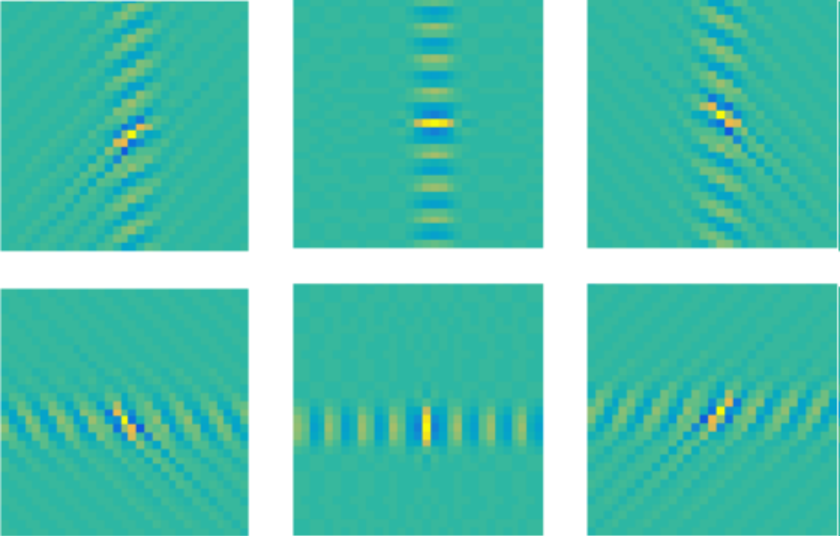
\includegraphics[width = .9\textwidth]{feasible_mi_time.pdf}
\end{minipage}
\caption{Left: $|m_i|,\, i = 1,\cdots,6$, right:$|\mathcal{F}^{-1}m_i|$}
\label{fig: m_i}
\end{figure}
\end{comment}

\section{Conclusion and future work}\label{sec: end}
In this paper, we consider directional wavelet schemes on dilated quincunx sub-lattice and analyze their regularity. We show that filters in bi-orthogonal bases have the same discontinuity in the frequency domain as that of the orthonormal bases at the corners of $C_0 = [-\pi/2,\pi/2)\times[-\pi/2,\pi/2)$. 

%Our analysis is closely related to our proposed bases construction algorithms, 
%and we show that the construction method of orthonormal bases can be easily extended to build frames construction of redundancy 2, which achieve much better time frequency localization and thus practically useful.
 We propose a different approach to construct biorthogonal wavelets from our previous approach for the orthonormal bases construction \cite{yin2014orthshear}. The directional dual filters $\widetilde{m_j}$ are first designed such that they can be extended to a bi-orthogonal frame and the remaining filters are obtained by solving linear systems and a constrained quadratic optimization derived from the identity summation and shift cancellation conditions for a biorthogonal MRA. We show numerically, that regularized dual wavelets $\widetilde{\psi^j}$ can be constructed, yet their corresponding wavelets $\psi^j$ are discontinuous in frequency domain, which is unavoidable according to our analysis.

The extension of the biorthogonal bases to low-redundancy dual frame construction is not studied here, which shall achieve at least the same regularity as that of the low-redundancy frame, but with more flexibility in the construction. In addition, our current bi-orthogonal wavelet construction algorithm may be extended to construct low-redundancy dual frames.
%\section{Conclusion and future work}\label{sec: end}
In this paper, we consider directional wavelet schemes on dilated quincunx sub-lattice and analyze their regularity. We show that filters in bi-orthogonal bases have the same discontinuity in the frequency domain as that of the orthonormal bases at the corners of $C_0 = [-\pi/2,\pi/2)\times[-\pi/2,\pi/2)$. 

%Our analysis is closely related to our proposed bases construction algorithms, 
%and we show that the construction method of orthonormal bases can be easily extended to build frames construction of redundancy 2, which achieve much better time frequency localization and thus practically useful.
 We propose a different approach to construct biorthogonal wavelets from our previous approach for the orthonormal bases construction \cite{yin2014orthshear}. The directional dual filters $\widetilde{m_j}$ are first designed such that they can be extended to a bi-orthogonal frame and the remaining filters are obtained by solving linear systems and a constrained quadratic optimization derived from the identity summation and shift cancellation conditions for a biorthogonal MRA. We show numerically, that regularized dual wavelets $\widetilde{\psi^j}$ can be constructed, yet their corresponding wavelets $\psi^j$ are discontinuous in frequency domain, which is unavoidable according to our analysis.

The extension of the biorthogonal bases to low-redundancy dual frame construction is not studied here, which shall achieve at least the same regularity as that of the low-redundancy frame, but with more flexibility in the construction. In addition, our current bi-orthogonal wavelet construction algorithm may be extended to construct low-redundancy dual frames.
%\section{Conclusion}\label{sec: end}

\newpage
\begin{appendices}
\section{Proof of Theorem \ref{thm: conds}}\label{app: cond-thm}
Take the Fourier transform of both sides of \eqref{eq: PR}, we have 
\begin{align*}
\sum_{\V{k}}\langle f,\phi_{\V{k}}\rangle\hat{\phi}(\V{\omega})e^{-i\V{\omega}^T\V{k}} = \sum_{\V{k}}&\langle f,\phi_{1,\V{k}}\rangle e^{-i\V{\omega}^T\V{D_2k}}|\V{D_2}|^{1/2}\hat{\phi}(\V{D_2}^T\V{\omega}) \\
&+ \sum_{j=1}^J\sum_{\V{k}}\langle f,\psi^j_{1,\V{k}}\rangle e^{-i\V{\omega}^T\V{Dk}}|\V{D}|^{1/2}\hat{\phi}(\V{D}^T\V{\omega})
\end{align*}
Suppose $m_j$ are trigonometric series
\begin{align}\label{eq: mra1}
m_0(\V{\omega}) = \sum_{\V{k}} c_{\V{k}}e^{-i \V{\omega}^T\V{k}} \hfill
m_j(\V{\omega}) = \sum_{\V{k}} g_{\V{k}}e^{-i \V{\omega}^T\V{k}},\quad j=1,\cdots,J
\end{align}
The first term on the right hand side can be represented by $\hat{\phi}(\V{\omega})$ and $\langle f,\phi_k\rangle$ using \eqref{eq: m0} and \eqref{eq: mra1}.

\begin{align*}
\text{the first term on R.H.S. } = \sum_{\V{k}}\langle f,\phi_{1,\V{k}}\rangle e^{-i\V{\omega}^T\V{D_2k}}|\V{D_2}|^{1/2}m_0(\V{\omega})\hat{\phi}(\V{\omega}) \\= \sum_{\V{k}}\Big(\sum_{\V{k}'}\langle f,\phi_{\V{k}'}\rangle\overline{c_{\V{k'-D_2k}}}|\V{D_2}|^{1/2}\Big)e^{-i\V{\omega}^T\V{D_2k}}|\V{D_2}|^{1/2}m_0(\V{\omega})\hat{\phi}(\V{\omega})\\
=\sum_{\V{k}'}\langle f,\phi_{\V{k}'}\rangle\Big(|\V{D_2}|\sum_{\V{k}}\overline{c_{\V{k'-D_2k}}}e^{i\V{\omega}^T(\V{k'-D_2k})}\Big)e^{-i\V{\omega} ^T\V{k}'} m_0(\V{\omega})\hat{\phi}(\V{\omega}).
\end{align*}
{\it Remark}.
If we have a shift $\V{k}_0$ in the down-sample scheme, i.e. $\V{D_2}\mathbb{Z}^2 - \V{k}_0$ instead of $\V{D_2}\mathbb{Z}^2$, so that we obtain coefficient of $\tilde{\phi}_{1,\V{k}} = \phi_{1,\V{k}+\V{k}_0}$ instead of $\phi_{1,\V{k}}$, and $\tilde{\phi}_1(\V{x}) =\phi_1(\V{x}-\V{k}_0)= |\V{D_2}|^{1/2}\sum_{\V{k}}c_{\V{k}}\phi(\V{x-k-k}_0) = |\V{D_2}|^{1/2}\sum_{\V{k}}c_{\V{k}-\V{k}_0}\phi(\V{x-k})$. This change of down-sample scheme results in an extra phase term $e^{-i\V{\omega}^T \V{k}_0}$ in $m_0$. Here, we use the down-sample scheme without translation.

Since $\bigcup_{\V{\beta}\in B} \{\V{\beta}\} :=\bigcup_{\V{\beta}\in B}(\V{D_2}\mathbb{Z}^2+\V{\beta}) = \mathbb{Z}^2$, where $B = \{ (0,0),\,(1,0),\,(0,1),\,(1,1)\}$, the summation over $\V{k}'\in \mathbb{Z}^2$ can be written as a double sum $\sum_{\V{\beta}\in B}\sum_{\V{k}'\in \{\V{\beta}\}}$,
\begin{align*}
\sum_{\V{\beta}\in B}\sum_{\V{k}'\in\{\V{\beta}\}} \langle f,\phi_{\V{k}'}\rangle\sum_{\V{k}}\overline{c_{\V{k'-D_2k}}}e^{i\V{\omega}^T(\V{k}'-\V{D_2k})}e^{-i\V{\omega}^T\V{k}'}|\V{D_2}|m_0(\V{\omega})\hat{\phi}(\V{\omega})\\
=\sum_{\V{\beta}\in B}\sum_{\V{k}'\in\{\V{\beta}\}} \langle f,\phi_{\V{k}'}\rangle\sum_{\V{k}\in\{\V{\beta}\}}\overline{c_{\V{k}}}e^{i\V{\omega}^T\V{k}}e^{-i\V{\omega}^T\V{k}'}|\V{D_2}|m_0(\V{\omega})\hat{\phi}(\V{\omega})
\end{align*}
The summation over $\V{k}$ in the middle is similar to the trigonometric form of $m_0$ in \eqref{eq: mra1}, but $\V{k}$ takes value on the shifted sub-lattice $\{\V{\beta}\}$ instead of $\mathbb{Z}^2$. Therefore, the summation equals to instead a linear combination of $m_0$ with shifts $\Gamma_0$,
\begin{align}\label{eq:eq1}
\sum_{\V{\pi}\in\Gamma_0}m_0(\V{\omega}+\V{\pi})\;e^{i\V{\beta}^T\V{\pi}} = \sum_{\V{k}\in \{\V{\beta}\}}c_{\V{k}}e^{-i\V{\omega}^T\V{k}}
\end{align}
Substitute \eqref{eq:eq1} into the previous expression,
\begin{align*}
\sum_{\V{\beta}\in B}\sum_{\V{k}'\in \{\V{\beta}\}}\langle f,\phi_{\V{k}'}\rangle\sum_{\V{\pi}\in\Gamma_0}\overline{m_0(\V{\omega}+\V{\pi})\;}e^{-i\V{\beta}^T\V{\pi}}\,e^{-i\V{\omega}^T\V{k}'}m_0(\V{\omega})\hat{\phi}(\V{\omega})
\end{align*}
Since $e^{i \V{\pi}^{T}\V{\beta}}=e^{i\V{\pi}^T\V{k}'},\; \forall \V{k}'\in \{\V{\beta}\} $, after rewriting the double sum over $\V{k}'$ back to a unit sum on $\mathbb{Z}^2$, we get
\begin{align*}
\sum_{\V{k}'}\langle f,\phi_{\V{k}'}\rangle e^{-i\V{\omega} ^T\V{k}'}\hat{\phi}(\V{\omega})\Big(\sum_{\V{\pi}\in\Gamma_0}\overline{m_0(\V{\omega}+\V{\pi})}m_0(\V{\omega})e^{-i\V{\pi}^T\V{k}'} \Big)
\end{align*}

Similarly, the second term on the R.H.S. of \eqref{eq: PR} equals to 
\begin{align*}
\sum_{j=1}^J\sum_{\V{k}'}\langle f,\phi_{\V{k}'}\rangle e^{-i\V{\omega}^T \V{k}'}\hat{\phi}(\V{\omega})\Big(\sum_{\V{\pi}\in\Gamma_1} \overline{m_j(\V{\omega}+\V{\pi})}m_j(\V{\omega})e^{-i\V{\pi}^T\V{k}'} \Big)
\end{align*}
(For Theorem \ref{thm: frame-conds} on frame construction, the summation of shifts $\V{\pi}$ is over $\Gamma_0$ instead of $\Gamma_1$.) 
Combining the two terms on the R.H.S. of \eqref{eq: PR}, and compare the coefficients of $\langle f,\phi_{\V{k}'}\rangle e^{-i\V{\omega}^T \V{k}'}\hat{\phi}(\V{\omega})$ on both sides, the perfect reconstruction condition is then equivalent to $\forall \V{k}'$,
\begin{align*}
\sum_{\V{\pi}\in\Gamma_0}e^{-i\V{\pi}^T\V{k}'}\overline{m_0(\V{\omega}+\V{\pi})}m_0(\V{\omega}) + \sum_j\sum_{\V{\pi}\in\Gamma_1} e^{-i\V{\pi}^T\V{k}'}\overline{m_j(\V{\omega}+\V{\pi})}m_j(\V{\omega}) = 1. 
%\sum_{l=0}^{3}e^{-i\gamma_l^T(k'-k_0)}\overline{M_0(\xi+\gamma_l)}M_0(\xi) + \sum_j\sum_{s=0}^7 e^{-i\nu_s^T(k'-k_j)}\overline{M_j(\xi+\nu_s)}M_j(\xi) = 1. 
\end{align*} 
This is equivalent to 
\begin{align*}
&|m_0(\V{\omega})|^2 + \sum_j|m_j(\V{\omega})|^2 = 1
\end{align*}
and
\begin{align*}
\sum_{j=0}^J\overline{m_j(\V{\omega}+\V{\pi})}m_j(\V{\omega}) = 0, 
%+ \overline{m_0(\V{\omega}+\V{\pi})}m_0(\V{\omega}) = 0, 
\,\V{\pi}\in \Gamma_0\setminus\{\V{0}\}\\
\sum_{j=1}^J\overline{m_j(\V{\omega}+\V{\pi})}m_j(\V{\omega}) = 0,\,\V{\pi}\in \Gamma_1\setminus \Gamma_0
\end{align*}

{\it Remark}.
Because each $m_j$ is $(2\pi,2\pi)$ periodic, we only need to check the above equality $\forall \V{\omega}\in S_0$.
If we downsample $\psi_1^j$ on a shifted sub-lattice $\V{D}\mathbb{Z}^2-\V{k}_j$, we then have an extra phase $e^{i\V{\pi}^T\V{k}_j}$ before $\overline{m_j(\V{\omega}+\V{\pi})}m_j(\V{\omega})$ in shift cancellation condition. This provides additional freedom in the construction yet it is not substantial.

\section{Lemmas}\label{app: lemmas}

\begin{lemma}\label{lem: null-space}
Let $\V{P}\in\mathbb{C}^{n\times n}$ be a projection matrix of rank $2$ and $\V{a},\V{b},\V{a}',\V{b}'\in\mathbb{C}^n,\, s.t.\, \V{a}^*\V{b} = (\V{a}')^*\V{b}'=1,\, \V{a}'^*\V{b} = \V{a}^*\V{b}' = \V{b}^*\V{b}' = 0.$ If $\V{P}(\V{I}_n - \V{a}\otimes\V{b} - \V{a}'\otimes\V{b}' ) = \V{0}$, then $\V{P}$ is the projection of $span\{\V{b},\V{b}'\}$.
\end{lemma}
\noindent{\it Proof.}
Since $$rank(\V{I}_n) \leq rank(\V{I}_n-\V{a}\otimes\V{b}-\V{a}'\otimes\V{b}') + rank(\V{a}\otimes\V{b}) + rank(\V{a}'\otimes\V{b}'),$$
it follows that $rank(\V{I}_n-\V{a}\otimes\V{b}-\V{a}'\otimes\V{b}')\geq n - 2$. On the other hand, because $rank(\V{P}) = 2$, $\V{P}(\V{I}_n - \V{a}\otimes\V{b} - \V{a}'\otimes\V{b}' ) = \V{0}$ implies that $rank(\V{I}_n-\V{a}\otimes\V{b}-\V{a}'\otimes\V{b}')\leq n - 2$. Hence $rank(\V{I}_n-\V{a}\otimes\V{b}-\V{a}'\otimes\V{b}') = n - 2$ and $\V{P}$ is the projection of $col(\V{I}_n-\V{a}\otimes\V{b}-\V{a}'\otimes\V{b}')^\bot$. On the other hand,
\begin{align*}
\V{b}^*(\V{I}_n-\V{a}\otimes\V{b}-\V{a}'\otimes\V{b}')
&= \V{b}^* - (\V{b}^*\V{a})\V{b}^* - (\V{b}^*\V{a}')(\V{b}')^*\\
&= \V{b}^* - \V{b}^* - 0\cdot (\V{b}')^* = \V{0}^*
\end{align*}
Therefore, $\V{P}\V{b} = \V{b}$.
Similarly, $(\V{b}')^* (\V{I}_n-\V{a}\otimes\V{b}-\V{a}'\otimes\V{b}')=\V{0}^*$ and $\V{P}\V{b}' = \V{b}'$. Moreover, as $\V{b}^*\V{b}' = 0$ and $rank(\V{P}) = 2$, $\V{P} = \Vert\V{b}\Vert^{-2}\cdot\V{b}\otimes\V{b} + \Vert\V{b}'\Vert^{-2}\cdot\V{b}'\otimes\V{b}'.$\qed

\begin{lemma}
Given $\M[:,-0](\V{\omega})$ is full rank $\forall \V{\omega}$, $\M[-0,:](\V{\omega})$ is singular if \eqref{eq: identity-cond} holds.
\end{lemma}
\noindent{\it Proof. }
If \eqref{eq: identity-cond} holds, then by Lemma \ref{lem: null-space}, $\meven,\,\modd$ are orthogonal to \\$col(\M[:,-0])$, therefore $\big[\,\modd,\meven,\M[:,-0]\,\big]\in\mathbb{C}^{8\times 8}$ is full rank. Due to \eqref{eq: identity-cond}, $\meven$ and $\mteven$ are not orthogonal to each other, hence $\big[\,\modd,\mteven,\M[:,-0]\,\big] = \big[\,\modd, \M\,\big]$ is full rank as well. Because $(\modd)^*\M[:, i] = 0,\,i= 0,\cdots,7$ and $\modd[-0]^*\M[-0, i] = (\modd)^*\M[:,i]$, $\modd[-0]$ is orthogonal to $col(\M[-0,:])$. Since $\big[ \modd[-0], \M[-0,:]\,\big]\in\mathbb{C}^{7\times 8}$ is full rank, $\M[-0,:]$ must be singular.\qed
\section{Supplementary Numerical Results}\label{app: supp-numerical}
\subsection{Numerical optimization of $\m{0}$ in 1D}
To test whether numerical optimization is a practical way to solve \eqref{eq: bi-orth-eq}, we first experiment on $m_0(\omega)$ and $\m{0}$ of pre-designed bi-orthogonal wavelets. We consider a low frequency filters corresponding to bi-orthogonal scaling functions $\phi,\, \tilde{\phi}$ with vanishing moments 3 and 5 respectively. 

\begin{wrapfigure}{r}{.4\textwidth}
\includegraphics[width = .4\textwidth]{filters.jpg}
\caption{1d filters, up: LoD, down: LoR}
\label{fig: filters}
\end{wrapfigure}
The filters are shown in Fig.\ref{fig: filters}. Suppose we know the upper decomposition filter, and we want to find the lower reconstruction filter by solving \eqref{eq: bi-orth-eq}, such that the filter has support as compact as possible. The corresponding $m_0$ and $\widetilde{m_0}$ are complex, yet we can shift the phase of $m_0$ such that $m_0$ is real and apply the same phase shift to $\m{0}$. Without loss of generality, \eqref{eq: bi-orth-eq} can be solved assuming that $m_0$ is  real.
It is not necessary that the corredponding $\widetilde{m_0}$ is also real, but in this testing case, $m_0(\V{\omega})$ and $\m{0}$ have the same phase, hence the phase-shifted $\m{0}$ is real as well. Fig.\ref{fig: m-funcs} shows the ground truth $m_0(\V{\omega})$ and $\m{0}$ considered in this simulation. %and in particular, $|m_0|$ is used as the known coefficients in \eqref{eq: bi-orth-eq}. Hereafter, we use $m_0(\omega)$ and $\m{0}$ to denote the real-valued functions.
\begin{figure}%{l}{.4\textwidth}
\begin{minipage}{.5\textwidth}
\includegraphics[width = \linewidth]{m-funcs.jpg}
\caption{$m_0(\V{\omega})$ and $\m{0}$}
\label{fig: m-funcs}
\end{minipage}
\hfill
\begin{minipage}{.4\textwidth}
\includegraphics[width = \textwidth]{1d-m-compare.jpg}\\
\includegraphics[width = \textwidth]{1d-filter-compare.jpg}
\caption{$\mhat{0}$ vs. $\m{0}$}
\label{fig: 1d-compare}
\end{minipage}
\end{figure}

Let $\mhat{0}$ be the approximation of $\m{0}$, which is solution of the following optimization problem
\begin{align}
\min_{\xvec}\; \Vert \V{D}\xvec\Vert^2 + \Vert \xvec\Vert^2,\quad s.t. \; \V{A}\xvec = \mathbf{1} \label{eq: opt-1d}
\end{align}
where $\V{A}$ in the constraint is the matrix generated from \eqref{eq: identity-cond} (in 1D, only a single shift of $\pi$ appears in the condition, so each row of $\V{A}$ has two non-zero entries). Notice that no symmetry constraint is imposed here, nevertheless, the solution shown in Fig.\ref{fig: 1d-compare} is almost symmetric. On the other hand, its support in the time domain is not as compact as that of $\m{0}$, see the bottom of Fig.\ref{fig: 1d-compare}.

\subsection{Numerical optimization of $\m{0}$ in 2D}
\begin{minipage}[c]{.45\textwidth}
\centering
\includegraphics[width = \textwidth]{2d-m-compare-1.jpg}
\captionof{figure}{Left: result of \eqref{eq: opt-1d} in 2D, Right: target}
\label{fig: 2d-compare-1}
\end{minipage}
\hfill
\begin{minipage}[c]{.5\textwidth}
The 2D case is much harder and several different optimization problems are formulated and their solutions are shown in the following. The 2D bi-orthogonal low-pass filters used here are the tensor products of the 1D filters used above.
{\it 2D version of \eqref{eq: opt-1d}}\\
 The 1D formulation can be easily extended to 2D, where $\V{D} = [\V{D}_x,\V{D}_y]$ consider 1st order derivative in both $x$ and $y$ directions, and $\V{A}$ is generated from \eqref{eq: identity-cond}, each row has four non-zero entries. Fig.\ref{fig: 2d-compare-1} shows the minimizer and compares it with the target function. It is obvious that the solution is not $90^\circ$-rotation invariant. Even worse is the fact that there is much energy in the vertical high-frequency domain.
\end{minipage}
\\[1em]
%{\it weighted L2 norm (Modulation Space$^{[\ref{app: modulation}]}$)}\\
To enforce the support of $\mhat{0}$ concentrates within the low frequency domain, the squared $\ell_2$-norm regulator in \eqref{eq: opt-1d} is changed to a weighted version (corresponding to Modulation space) as follows,
\begin{align}
\min_{\xvec}\; \Vert\V{ D}\xvec\Vert^2 + \lambda\Vert \wvec\circ\xvec\Vert^2,\quad s.t. \; \V{A}\xvec = \mathbf{1} \label{eq: opt-2d-weight}
\end{align} 
where $\circ$ is Hadamard product and $\wvec$ is a weight vector. In particular, we choose $\forall \omega, \; \wvec(\V{\omega}) = \Vert\V{\omega}\Vert$. Fig.\ref{fig: 2d-compare-2} and Fig.\ref{fig: 2d-compare-2.2} show the minimizer of \eqref{eq: opt-2d-weight} with $\lambda=60$ and $600$ respectively. As $\lambda$ increases, the support of the minimizer concentrates more within the low frequency region. As shown in Fig.\ref{fig: 2d-compare-2}, when $\lambda$ is not huge, the minimizer achieves a certain level of but not full symmetry, whereas Fig.\ref{fig: 2d-compare-2.2} shows that huge $\lambda$ imposes full symmetry.

\begin{minipage}{.9\textwidth}
\centering
\includegraphics[width = .9\textwidth]{2d-m-compare-2-1-eps-converted-to.pdf}\\
\includegraphics[width = .9\textwidth]{2d-filter-compare-2-1-eps-converted-to.pdf}
\captionof{figure}{result of \eqref{eq: opt-2d-weight} $\mhat{0}$ ($\lambda = 60$), target $\m{0}$ and their difference, Top: frequency domain, Bottom: time domain}
\label{fig: 2d-compare-2}
\end{minipage}

\vspace*{2em}
\begin{minipage}{.9\textwidth}
\centering
\includegraphics[width = .9\textwidth]{2d-m-compare-2-2-eps-converted-to.pdf}\\
\includegraphics[width = .9\textwidth]{2d-filter-compare-2-2-eps-converted-to.pdf}
\captionof{figure}{result of \eqref{eq: opt-2d-weight} $\mhat{0}$ ($\lambda = 600$), target $\m{0}$ and their difference}
\label{fig: 2d-compare-2.2}
\end{minipage}
\\[1em]
{\it weighted L2 norm with symmetry constraint}\\
If we hard constrain the symmetry by the following
\begin{align}
\min_{\xvec}\; \Vert \V{D}\xvec\Vert^2 + \lambda\Vert \wvec\circ\xvec\Vert^2,\quad s.t. \; \V{A}\xvec = \mathbf{1},\,\V{S}\xvec = \mathbf{0} \label{eq: opt-2d-weight-sym}
\end{align}
where each row of $\V{S}$ has an one entry and a negative one entry at the location of two points have the same value due to symmetry. In practice, we put symmetry constraints such that the upper half plane is symmetric to the lower half plane w.r.t. $x$ coordinate and the first quadrant is $90^{\circ}-$ rotational invariant w.r.t. the second quadrant. The symmetry constraint makes the optimization problem significantly harder, resulting in longer optimization algorithm running time and no near-optimal solution is found (the algorithm terminates as the maximum number of iterations is exceeded). Fig.\ref{fig: 2d-compare-3} shows the result provided by the Matlab quadratic minimization solver, unfortunately, there are artifacts at the near endpoints of $x$ and $y$ coordinates.
\begin{figure}[h]
\includegraphics[width = .9\textwidth]{2d-m-compare-3-eps-converted-to.pdf}\\
\includegraphics[width = .9\textwidth]{2d-m-compare-3-2-eps-converted-to.pdf}
\caption{solution of \eqref{eq: opt-2d-weight-sym} (top: $\lambda=60$, bottom: $\lambda=600$) provided by Matlab solver \texttt{quadprog}}
\label{fig: 2d-compare-3}
\end{figure}
\\
On the other hand, asymmetric solution can always be symmetrized by the average of the solution and its dual
w.r.t. rotation, mirroring, etc. This approach increase the support of the solution, thus a well concentrated solution in the frequency domain is necessary to begin with.
\\[1em]
{\it Other potential formulations}\\
We may also putting weights in the first L2-norm of derivatives, such that
\begin{align}
\min_{\xvec}\; \Vert \wvec'\circ \V{D}\xvec\Vert^2 + \lambda\Vert \wvec\circ\xvec\Vert^2,\quad s.t. \; \V{A}\xvec = \mathbf{1} \label{eq: opt-2d-double-weight}
\end{align}
Clearly, $\wvec'(\V{\omega})\rightarrow +\infty$ as $|\V{\omega}|\rightarrow +\infty$, but its behavior near the origin is unclear.
%\section{Proof of Theorem \ref{thm: conds}}\label{app: cond-thm}
Take the Fourier transform of both sides of \eqref{eq: PR}, we have 
\begin{align*}
\sum_{\V{k}}\langle f,\phi_{\V{k}}\rangle\hat{\phi}(\V{\omega})e^{-i\V{\omega}^T\V{k}} = \sum_{\V{k}}&\langle f,\phi_{1,\V{k}}\rangle e^{-i\V{\omega}^T\V{D_2k}}|\V{D_2}|^{1/2}\hat{\phi}(\V{D_2}^T\V{\omega}) \\
&+ \sum_{j=1}^J\sum_{\V{k}}\langle f,\psi^j_{1,\V{k}}\rangle e^{-i\V{\omega}^T\V{Dk}}|\V{D}|^{1/2}\hat{\phi}(\V{D}^T\V{\omega})
\end{align*}
Suppose $m_j$ are trigonometric series
\begin{align}\label{eq: mra1}
m_0(\V{\omega}) = \sum_{\V{k}} c_{\V{k}}e^{-i \V{\omega}^T\V{k}} \hfill
m_j(\V{\omega}) = \sum_{\V{k}} g_{\V{k}}e^{-i \V{\omega}^T\V{k}},\quad j=1,\cdots,J
\end{align}
The first term on the right hand side can be represented by $\hat{\phi}(\V{\omega})$ and $\langle f,\phi_k\rangle$ using \eqref{eq: m0} and \eqref{eq: mra1}.

\begin{align*}
\text{the first term on R.H.S. } = \sum_{\V{k}}\langle f,\phi_{1,\V{k}}\rangle e^{-i\V{\omega}^T\V{D_2k}}|\V{D_2}|^{1/2}m_0(\V{\omega})\hat{\phi}(\V{\omega}) \\= \sum_{\V{k}}\Big(\sum_{\V{k}'}\langle f,\phi_{\V{k}'}\rangle\overline{c_{\V{k'-D_2k}}}|\V{D_2}|^{1/2}\Big)e^{-i\V{\omega}^T\V{D_2k}}|\V{D_2}|^{1/2}m_0(\V{\omega})\hat{\phi}(\V{\omega})\\
=\sum_{\V{k}'}\langle f,\phi_{\V{k}'}\rangle\Big(|\V{D_2}|\sum_{\V{k}}\overline{c_{\V{k'-D_2k}}}e^{i\V{\omega}^T(\V{k'-D_2k})}\Big)e^{-i\V{\omega} ^T\V{k}'} m_0(\V{\omega})\hat{\phi}(\V{\omega}).
\end{align*}
{\it Remark}.
If we have a shift $\V{k}_0$ in the down-sample scheme, i.e. $\V{D_2}\mathbb{Z}^2 - \V{k}_0$ instead of $\V{D_2}\mathbb{Z}^2$, so that we obtain coefficient of $\tilde{\phi}_{1,\V{k}} = \phi_{1,\V{k}+\V{k}_0}$ instead of $\phi_{1,\V{k}}$, and $\tilde{\phi}_1(\V{x}) =\phi_1(\V{x}-\V{k}_0)= |\V{D_2}|^{1/2}\sum_{\V{k}}c_{\V{k}}\phi(\V{x-k-k}_0) = |\V{D_2}|^{1/2}\sum_{\V{k}}c_{\V{k}-\V{k}_0}\phi(\V{x-k})$. This change of down-sample scheme results in an extra phase term $e^{-i\V{\omega}^T \V{k}_0}$ in $m_0$. Here, we use the down-sample scheme without translation.

Since $\bigcup_{\V{\beta}\in B} \{\V{\beta}\} :=\bigcup_{\V{\beta}\in B}(\V{D_2}\mathbb{Z}^2+\V{\beta}) = \mathbb{Z}^2$, where $B = \{ (0,0),\,(1,0),\,(0,1),\,(1,1)\}$, the summation over $\V{k}'\in \mathbb{Z}^2$ can be written as a double sum $\sum_{\V{\beta}\in B}\sum_{\V{k}'\in \{\V{\beta}\}}$,
\begin{align*}
\sum_{\V{\beta}\in B}\sum_{\V{k}'\in\{\V{\beta}\}} \langle f,\phi_{\V{k}'}\rangle\sum_{\V{k}}\overline{c_{\V{k'-D_2k}}}e^{i\V{\omega}^T(\V{k}'-\V{D_2k})}e^{-i\V{\omega}^T\V{k}'}|\V{D_2}|m_0(\V{\omega})\hat{\phi}(\V{\omega})\\
=\sum_{\V{\beta}\in B}\sum_{\V{k}'\in\{\V{\beta}\}} \langle f,\phi_{\V{k}'}\rangle\sum_{\V{k}\in\{\V{\beta}\}}\overline{c_{\V{k}}}e^{i\V{\omega}^T\V{k}}e^{-i\V{\omega}^T\V{k}'}|\V{D_2}|m_0(\V{\omega})\hat{\phi}(\V{\omega})
\end{align*}
The summation over $\V{k}$ in the middle is similar to the trigonometric form of $m_0$ in \eqref{eq: mra1}, but $\V{k}$ takes value on the shifted sub-lattice $\{\V{\beta}\}$ instead of $\mathbb{Z}^2$. Therefore, the summation equals to instead a linear combination of $m_0$ with shifts $\Gamma_0$,
\begin{align}\label{eq:eq1}
\sum_{\V{\pi}\in\Gamma_0}m_0(\V{\omega}+\V{\pi})\;e^{i\V{\beta}^T\V{\pi}} = \sum_{\V{k}\in \{\V{\beta}\}}c_{\V{k}}e^{-i\V{\omega}^T\V{k}}
\end{align}
Substitute \eqref{eq:eq1} into the previous expression,
\begin{align*}
\sum_{\V{\beta}\in B}\sum_{\V{k}'\in \{\V{\beta}\}}\langle f,\phi_{\V{k}'}\rangle\sum_{\V{\pi}\in\Gamma_0}\overline{m_0(\V{\omega}+\V{\pi})\;}e^{-i\V{\beta}^T\V{\pi}}\,e^{-i\V{\omega}^T\V{k}'}m_0(\V{\omega})\hat{\phi}(\V{\omega})
\end{align*}
Since $e^{i \V{\pi}^{T}\V{\beta}}=e^{i\V{\pi}^T\V{k}'},\; \forall \V{k}'\in \{\V{\beta}\} $, after rewriting the double sum over $\V{k}'$ back to a unit sum on $\mathbb{Z}^2$, we get
\begin{align*}
\sum_{\V{k}'}\langle f,\phi_{\V{k}'}\rangle e^{-i\V{\omega} ^T\V{k}'}\hat{\phi}(\V{\omega})\Big(\sum_{\V{\pi}\in\Gamma_0}\overline{m_0(\V{\omega}+\V{\pi})}m_0(\V{\omega})e^{-i\V{\pi}^T\V{k}'} \Big)
\end{align*}

Similarly, the second term on the R.H.S. of \eqref{eq: PR} equals to 
\begin{align*}
\sum_{j=1}^J\sum_{\V{k}'}\langle f,\phi_{\V{k}'}\rangle e^{-i\V{\omega}^T \V{k}'}\hat{\phi}(\V{\omega})\Big(\sum_{\V{\pi}\in\Gamma_1} \overline{m_j(\V{\omega}+\V{\pi})}m_j(\V{\omega})e^{-i\V{\pi}^T\V{k}'} \Big)
\end{align*}
(For Theorem \ref{thm: frame-conds} on frame construction, the summation of shifts $\V{\pi}$ is over $\Gamma_0$ instead of $\Gamma_1$.) 
Combining the two terms on the R.H.S. of \eqref{eq: PR}, and compare the coefficients of $\langle f,\phi_{\V{k}'}\rangle e^{-i\V{\omega}^T \V{k}'}\hat{\phi}(\V{\omega})$ on both sides, the perfect reconstruction condition is then equivalent to $\forall \V{k}'$,
\begin{align*}
\sum_{\V{\pi}\in\Gamma_0}e^{-i\V{\pi}^T\V{k}'}\overline{m_0(\V{\omega}+\V{\pi})}m_0(\V{\omega}) + \sum_j\sum_{\V{\pi}\in\Gamma_1} e^{-i\V{\pi}^T\V{k}'}\overline{m_j(\V{\omega}+\V{\pi})}m_j(\V{\omega}) = 1. 
%\sum_{l=0}^{3}e^{-i\gamma_l^T(k'-k_0)}\overline{M_0(\xi+\gamma_l)}M_0(\xi) + \sum_j\sum_{s=0}^7 e^{-i\nu_s^T(k'-k_j)}\overline{M_j(\xi+\nu_s)}M_j(\xi) = 1. 
\end{align*} 
This is equivalent to 
\begin{align*}
&|m_0(\V{\omega})|^2 + \sum_j|m_j(\V{\omega})|^2 = 1
\end{align*}
and
\begin{align*}
\sum_{j=0}^J\overline{m_j(\V{\omega}+\V{\pi})}m_j(\V{\omega}) = 0, 
%+ \overline{m_0(\V{\omega}+\V{\pi})}m_0(\V{\omega}) = 0, 
\,\V{\pi}\in \Gamma_0\setminus\{\V{0}\}\\
\sum_{j=1}^J\overline{m_j(\V{\omega}+\V{\pi})}m_j(\V{\omega}) = 0,\,\V{\pi}\in \Gamma_1\setminus \Gamma_0
\end{align*}

{\it Remark}.
Because each $m_j$ is $(2\pi,2\pi)$ periodic, we only need to check the above equality $\forall \V{\omega}\in S_0$.
If we downsample $\psi_1^j$ on a shifted sub-lattice $\V{D}\mathbb{Z}^2-\V{k}_j$, we then have an extra phase $e^{i\V{\pi}^T\V{k}_j}$ before $\overline{m_j(\V{\omega}+\V{\pi})}m_j(\V{\omega})$ in shift cancellation condition. This provides additional freedom in the construction yet it is not substantial.

%\section{Supplementary Numerical Results}\label{app: supp-numerical}
\subsection{Numerical optimization of $\m{0}$ in 1D}
To test whether numerical optimization is a practical way to solve \eqref{eq: bi-orth-eq}, we first experiment on $m_0(\omega)$ and $\m{0}$ of pre-designed bi-orthogonal wavelets. We consider a low frequency filters corresponding to bi-orthogonal scaling functions $\phi,\, \tilde{\phi}$ with vanishing moments 3 and 5 respectively. 

\begin{wrapfigure}{r}{.4\textwidth}
\includegraphics[width = .4\textwidth]{filters.jpg}
\caption{1d filters, up: LoD, down: LoR}
\label{fig: filters}
\end{wrapfigure}
The filters are shown in Fig.\ref{fig: filters}. Suppose we know the upper decomposition filter, and we want to find the lower reconstruction filter by solving \eqref{eq: bi-orth-eq}, such that the filter has support as compact as possible. The corresponding $m_0$ and $\widetilde{m_0}$ are complex, yet we can shift the phase of $m_0$ such that $m_0$ is real and apply the same phase shift to $\m{0}$. Without loss of generality, \eqref{eq: bi-orth-eq} can be solved assuming that $m_0$ is  real.
It is not necessary that the corredponding $\widetilde{m_0}$ is also real, but in this testing case, $m_0(\V{\omega})$ and $\m{0}$ have the same phase, hence the phase-shifted $\m{0}$ is real as well. Fig.\ref{fig: m-funcs} shows the ground truth $m_0(\V{\omega})$ and $\m{0}$ considered in this simulation. %and in particular, $|m_0|$ is used as the known coefficients in \eqref{eq: bi-orth-eq}. Hereafter, we use $m_0(\omega)$ and $\m{0}$ to denote the real-valued functions.
\begin{figure}%{l}{.4\textwidth}
\begin{minipage}{.5\textwidth}
\includegraphics[width = \linewidth]{m-funcs.jpg}
\caption{$m_0(\V{\omega})$ and $\m{0}$}
\label{fig: m-funcs}
\end{minipage}
\hfill
\begin{minipage}{.4\textwidth}
\includegraphics[width = \textwidth]{1d-m-compare.jpg}\\
\includegraphics[width = \textwidth]{1d-filter-compare.jpg}
\caption{$\mhat{0}$ vs. $\m{0}$}
\label{fig: 1d-compare}
\end{minipage}
\end{figure}

Let $\mhat{0}$ be the approximation of $\m{0}$, which is solution of the following optimization problem
\begin{align}
\min_{\xvec}\; \Vert \V{D}\xvec\Vert^2 + \Vert \xvec\Vert^2,\quad s.t. \; \V{A}\xvec = \mathbf{1} \label{eq: opt-1d}
\end{align}
where $\V{A}$ in the constraint is the matrix generated from \eqref{eq: identity-cond} (in 1D, only a single shift of $\pi$ appears in the condition, so each row of $\V{A}$ has two non-zero entries). Notice that no symmetry constraint is imposed here, nevertheless, the solution shown in Fig.\ref{fig: 1d-compare} is almost symmetric. On the other hand, its support in the time domain is not as compact as that of $\m{0}$, see the bottom of Fig.\ref{fig: 1d-compare}.

\subsection{Numerical optimization of $\m{0}$ in 2D}
\begin{minipage}[c]{.45\textwidth}
\centering
\includegraphics[width = \textwidth]{2d-m-compare-1.jpg}
\captionof{figure}{Left: result of \eqref{eq: opt-1d} in 2D, Right: target}
\label{fig: 2d-compare-1}
\end{minipage}
\hfill
\begin{minipage}[c]{.5\textwidth}
The 2D case is much harder and several different optimization problems are formulated and their solutions are shown in the following. The 2D bi-orthogonal low-pass filters used here are the tensor products of the 1D filters used above.
{\it 2D version of \eqref{eq: opt-1d}}\\
 The 1D formulation can be easily extended to 2D, where $\V{D} = [\V{D}_x,\V{D}_y]$ consider 1st order derivative in both $x$ and $y$ directions, and $\V{A}$ is generated from \eqref{eq: identity-cond}, each row has four non-zero entries. Fig.\ref{fig: 2d-compare-1} shows the minimizer and compares it with the target function. It is obvious that the solution is not $90^\circ$-rotation invariant. Even worse is the fact that there is much energy in the vertical high-frequency domain.
\end{minipage}
\\[1em]
%{\it weighted L2 norm (Modulation Space$^{[\ref{app: modulation}]}$)}\\
To enforce the support of $\mhat{0}$ concentrates within the low frequency domain, the squared $\ell_2$-norm regulator in \eqref{eq: opt-1d} is changed to a weighted version (corresponding to Modulation space) as follows,
\begin{align}
\min_{\xvec}\; \Vert\V{ D}\xvec\Vert^2 + \lambda\Vert \wvec\circ\xvec\Vert^2,\quad s.t. \; \V{A}\xvec = \mathbf{1} \label{eq: opt-2d-weight}
\end{align} 
where $\circ$ is Hadamard product and $\wvec$ is a weight vector. In particular, we choose $\forall \omega, \; \wvec(\V{\omega}) = \Vert\V{\omega}\Vert$. Fig.\ref{fig: 2d-compare-2} and Fig.\ref{fig: 2d-compare-2.2} show the minimizer of \eqref{eq: opt-2d-weight} with $\lambda=60$ and $600$ respectively. As $\lambda$ increases, the support of the minimizer concentrates more within the low frequency region. As shown in Fig.\ref{fig: 2d-compare-2}, when $\lambda$ is not huge, the minimizer achieves a certain level of but not full symmetry, whereas Fig.\ref{fig: 2d-compare-2.2} shows that huge $\lambda$ imposes full symmetry.

\begin{minipage}{.9\textwidth}
\centering
\includegraphics[width = .9\textwidth]{2d-m-compare-2-1-eps-converted-to.pdf}\\
\includegraphics[width = .9\textwidth]{2d-filter-compare-2-1-eps-converted-to.pdf}
\captionof{figure}{result of \eqref{eq: opt-2d-weight} $\mhat{0}$ ($\lambda = 60$), target $\m{0}$ and their difference, Top: frequency domain, Bottom: time domain}
\label{fig: 2d-compare-2}
\end{minipage}

\vspace*{2em}
\begin{minipage}{.9\textwidth}
\centering
\includegraphics[width = .9\textwidth]{2d-m-compare-2-2-eps-converted-to.pdf}\\
\includegraphics[width = .9\textwidth]{2d-filter-compare-2-2-eps-converted-to.pdf}
\captionof{figure}{result of \eqref{eq: opt-2d-weight} $\mhat{0}$ ($\lambda = 600$), target $\m{0}$ and their difference}
\label{fig: 2d-compare-2.2}
\end{minipage}
\\[1em]
{\it weighted L2 norm with symmetry constraint}\\
If we hard constrain the symmetry by the following
\begin{align}
\min_{\xvec}\; \Vert \V{D}\xvec\Vert^2 + \lambda\Vert \wvec\circ\xvec\Vert^2,\quad s.t. \; \V{A}\xvec = \mathbf{1},\,\V{S}\xvec = \mathbf{0} \label{eq: opt-2d-weight-sym}
\end{align}
where each row of $\V{S}$ has an one entry and a negative one entry at the location of two points have the same value due to symmetry. In practice, we put symmetry constraints such that the upper half plane is symmetric to the lower half plane w.r.t. $x$ coordinate and the first quadrant is $90^{\circ}-$ rotational invariant w.r.t. the second quadrant. The symmetry constraint makes the optimization problem significantly harder, resulting in longer optimization algorithm running time and no near-optimal solution is found (the algorithm terminates as the maximum number of iterations is exceeded). Fig.\ref{fig: 2d-compare-3} shows the result provided by the Matlab quadratic minimization solver, unfortunately, there are artifacts at the near endpoints of $x$ and $y$ coordinates.
\begin{figure}[h]
\includegraphics[width = .9\textwidth]{2d-m-compare-3-eps-converted-to.pdf}\\
\includegraphics[width = .9\textwidth]{2d-m-compare-3-2-eps-converted-to.pdf}
\caption{solution of \eqref{eq: opt-2d-weight-sym} (top: $\lambda=60$, bottom: $\lambda=600$) provided by Matlab solver \texttt{quadprog}}
\label{fig: 2d-compare-3}
\end{figure}
\\
On the other hand, asymmetric solution can always be symmetrized by the average of the solution and its dual
w.r.t. rotation, mirroring, etc. This approach increase the support of the solution, thus a well concentrated solution in the frequency domain is necessary to begin with.
\\[1em]
{\it Other potential formulations}\\
We may also putting weights in the first L2-norm of derivatives, such that
\begin{align}
\min_{\xvec}\; \Vert \wvec'\circ \V{D}\xvec\Vert^2 + \lambda\Vert \wvec\circ\xvec\Vert^2,\quad s.t. \; \V{A}\xvec = \mathbf{1} \label{eq: opt-2d-double-weight}
\end{align}
Clearly, $\wvec'(\V{\omega})\rightarrow +\infty$ as $|\V{\omega}|\rightarrow +\infty$, but its behavior near the origin is unclear.
\end{appendices}

\bibliographystyle{IEEEtran}%bib/te}
\bibliography{ref}
\end{document}